% =====================================================================
% Dissertation main file — Oxford Mathematical Institute MScThesis template
% (MScThesis.cls, dept. template by J. Dewynne 2002, from ociamthesis v1.8).
% Migrated from ociamthesis.cls June 2026; structure unchanged.
% Build: latexmk -pdf main.tex
% Line spacing: \baselineskip=18pt on 12pt body ≥ the required 1.25 spacing
% (the template's own default, per the MSc guidelines).
% =====================================================================
\documentclass[12pt]{MScThesis}

%load any additional packages
\usepackage{amssymb}
\usepackage{amsmath}
\usepackage{booktabs}        % toprule / midrule / bottomrule
\usepackage{tabularx}        % flexible-width table columns
\usepackage{multirow}        % multi-row table cells (used in the Data chapter)
\usepackage[numbers]{natbib} % \citet, \citep used in the chapters
\usepackage{url}             % \url in bibliography entries
\usepackage{tikz}            % shard-loop diagram in chapter 2
\usetikzlibrary{positioning, arrows.meta}

% ---- placeholder macros (draft phase) --------------------------------
% Framed boxes that compile now and are swapped for the real artifact
% (figure PNG / generated table) once copied in from outputs/ on the
% data drive. Usage: \figplaceholder{label}{caption}{source-path}
\newcommand{\figplaceholder}[3]{%
\begin{figure}[htbp]\centering
\fbox{\parbox[c][5cm][c]{0.9\textwidth}{\centering
\textbf{[Figure placeholder]}\\[1.5ex]\small to insert from: \texttt{#3}}}
\caption{#2}\label{#1}
\end{figure}}
\newcommand{\tabplaceholder}[3]{%
\begin{table}[htbp]\centering
\fbox{\parbox[c][3cm][c]{0.9\textwidth}{\centering
\textbf{[Table placeholder]}\\[1.5ex]\small to insert from: \texttt{#3}}}
\caption{#2}\label{#1}
\end{table}}
\newcommand{\pendingnote}[1]{%
\noindent\fbox{\parbox{0.97\textwidth}{\textbf{[Pending]} #1}}\medskip}
% ----------------------------------------------------------------------

% The class's title-page crest points at crest.eps, which the department does
% not distribute; reuse the Oxford logo already in this folder instead.
\renewcommand{\crest}{\hbox to\textwidth{\hss
\includegraphics[width=35mm]{oxlogo}\hss}}

\title{Deep Learning Models of\\[1ex]
        Loan Portfolios and Asset-Backed Securities}

\author{Felipe Pombal Fritsch}
\college{Reuben College}

%\renewcommand{\submittedtext}{change the default text here if needed}
% NB: the class prefixes "A thesis submitted in partial fulfillment of the
% MSc in" — so \degree carries only the programme name.
\degree{Mathematical and Computational Finance}
\degreedate{Trinity 2026}

%end the preamble and start the document
\begin{document}

%this baselineskip gives sufficient line spacing for an examiner to easily
%markup the thesis with comments (≥ 1.25 spacing per the guidelines)
\baselineskip=18pt plus1pt

%set the number of sectioning levels that get numbered and appear in the contents
\setcounter{secnumdepth}{3}
\setcounter{tocdepth}{3}

\maketitle                  % title page from the preamble info
\begin{dedication}
% TODO — or delete the \begin{dedication}
% TODO — or delete the \begin{dedication}
% TODO — or delete the \include{dedication} line in main.tex if not wanted.
\end{dedication}
 line in main.tex if not wanted.
\end{dedication}
 line in main.tex if not wanted.
\end{dedication}

\begin{acknowledgements}
% TODO: supervisor, family, etc.
\end{acknowledgements}

\begin{abstract}
% TODO: ~1 page. Quarry: writeup/methodology/methodology_overview.tex (abstract
% + §1.1 contributions) once Phase 2/3 results are in.
\end{abstract}


\begin{romanpages}          % roman page numbering for front matter
\tableofcontents
\listoffigures
% ============================================================
%  Notation — front-matter reference page (June 2026 skeleton pass).
%  Included inside the romanpages block in main.tex, so it carries a
%  roman folio and is excluded from the 40-page body count. Every
%  symbol is rendered exactly as it appears in the body (chapters 1–5,
%  appendices A–C) and points to its defining equation; forward
%  \eqref references resolve into Chapters 1–2 after the usual reruns.
% ============================================================
\begin{alwayssingle}
\thispagestyle{plain}
\begin{center}
\vspace*{1.5cm}
{\Large \bfseries Notation}
\end{center}
\vspace{0.5cm}

\noindent
\begin{tabularx}{\textwidth}{@{}lX@{}}
\toprule
Symbol & Meaning \\
\midrule
\multicolumn{2}{@{}l}{\textit{Indices and sets}}\\[2pt]
$i,\ t$ & loan index; reporting (calendar) month \\
$\mathcal{P}$ & a pool --- a characteristic bucket or a random pool of loans \\
\addlinespace
\multicolumn{2}{@{}l}{\textit{State space}}\\[2pt]
$S_{i,t}\in\mathcal{S}$ & state of loan $i$ in month $t$; $|\mathcal{S}|=7$ states, four live origins (a $4\times7$ matrix) \\
\addlinespace
\multicolumn{2}{@{}l}{\textit{Model and estimation}}\\[2pt]
$x_{i,t}\in\mathbb{R}^{d}$ & covariate vector: current state, loan fields, macro block, seasonality \\
$p_\theta(j\mid x)$ & model's one-month transition probability, Eq.~\eqref{eq:object} \\
$\widehat{P}_{uv}$ & Laplace-smoothed empirical transition matrix, Eq.~\eqref{eq:empirical} \\
$w_i = 1/p$ & importance (Horvitz--Thompson) weight undoing class thinning, Eq.~\eqref{eq:weightednll} \\
$L,\ K$ & hidden-layer count (network depth), Eq.~\eqref{eq:mlp}; ensemble size ($K=8$) \\
$\mathrm{NLL}$ & out-of-sample mean negative log-likelihood, Eq.~\eqref{eq:nll} \\
\addlinespace
\multicolumn{2}{@{}l}{\textit{Derived covariates}}\\[2pt]
$\mathrm{incentive}_{i,t}$ & refinancing incentive $r^{\mathrm{cur}}_{i,t}-m(t)$, Eq.~\eqref{eq:incentive} \\
$\mathrm{ltv}^{\mathrm{mtm}}_{i,t}$ & mark-to-market LTV, Eq.~\eqref{eq:mtmltv} \\
\addlinespace
\multicolumn{2}{@{}l}{\textit{Backtest and roll-forward}}\\[2pt]
$\mathrm{shard}(i)$ & loan-keyed hash partition $h(\mathrm{LoanID}_i)\bmod N$, $N=256$, Eq.~\eqref{eq:shard} \\
$k$ & backtest window / test year, $k=2015,\dots,2025$; training cutoff $\mathrm{Dec}(k{-}2)$ \\
$\rho_h,\ H$ & rolled-forward state distribution, Eq.~\eqref{eq:rollforward}; horizon $H=12$ \\
$\widehat{C}_{\mathcal{P}},\ q_i$ & predicted pool event count, Eq.~\eqref{eq:poolcount}; per-loan horizon probability \\
\bottomrule
\end{tabularx}
\end{alwayssingle}
            % notation reference page (front matter, roman folio)
\end{romanpages}

%chapters
% ============================================================
%  Chapter 1 — Introduction
% ============================================================

\chapter{Introduction}
\label{chap:intro}

\section{The modelling object}
\label{sec:intro-object}

A mortgage is a small dynamical system.  In any month it occupies one
of a small number of \emph{states} --- it is current on its payments,
or 30, 60, or 90-plus days past due, or it has terminated through
prepayment or a credit event --- and between consecutive months it
moves between these states with probabilities that depend on the
loan's characteristics and the economic environment.  The cashflows
of any mortgage portfolio or mortgage-backed security are completely
determined by these movements: a prepayment returns principal early
(a risk to the investor when rates have fallen), while the path from
delinquency through foreclosure destroys value.  Modelling the
\emph{conditional transition distribution} is therefore the natural
primitive for both credit and prepayment risk.

Formally, let $S_{i,t}\in\mathcal{S}$ denote the state of loan $i$ in
month $t$, and let $x_{i,t}\in\mathbb{R}^{d}$ collect everything
observable about the loan and its environment at $t$.  The object of
interest is
\begin{equation}
\label{eq:object}
p_\theta\!\left(j \mid x_{i,t}\right) \;\approx\;
\mathbb{P}\!\left(S_{i,t+1}=j \,\middle|\, x_{i,t}\right),
\qquad j\in\mathcal{S},
\end{equation}
a multinomial classification of next month's state.  Every model in
this dissertation --- from a frequency-count transition matrix to an
ensemble of deep neural networks --- is an estimator of
\eqref{eq:object}; they differ only in how flexibly they allow the
probabilities to depend on the covariates.

The central empirical claim of \citet{sirignano2021}, which this
dissertation tests on a different and cleaner dataset, is that the
dependence of \eqref{eq:object} on $x$ is strongly \emph{nonlinear}
and features economically meaningful \emph{interactions} between
covariates.  Linear models misspecify this dependence, and the
misspecification compounds when loan-level probabilities are
aggregated to pool-level cashflows --- the level at which
mortgage-backed securities are priced.

Agency mortgage-backed securities are among the largest fixed-income markets in the world, and their value rests entirely on how the underlying loans move between paying, delinquency, default, and prepayment. For the investor, mispricing the speed of prepayment misstates both the timing of returned principal and the value of the embedded call; for the lender and the regulator, mispricing the path into default misstates capital and provisions. The stakes of the conditional transition distribution in \eqref{eq:object} are therefore not incidental to the modelling --- they are why a more faithful estimator is worth the effort.

This study sits at the confluence of two literatures. The first is the option-theoretic tradition in mortgage modelling, which treats prepayment and default as the exercise of embedded options driven by borrower incentives \citep{schwartz1989, deng2000}. The second is the turn to flexible machine learning in credit and asset pricing: that such models sharpen consumer credit-risk forecasts \citep{khandani2010}, that their flexibility carries distributional consequences in mortgage markets \citep{fuster2022}, and that nonlinear methods materially improve the measurement of expected returns where linear models fail \citep{gukellyxiu2020}. \citet{sirignano2021} bring these together for mortgage risk specifically, and it is their central claim --- that transition risk depends on covariates nonlinearly and interactively --- that this dissertation tests on a cleaner, fully reproducible dataset.

Two questions organise the work. Does the deep-learning advantage documented on subprime-heavy, private-label data survive in the prime conforming credit box, where credit events are rarer and relationships plausibly tamer? And across which regimes --- the COVID-era forbearance episode, the 2020--21 refinancing wave, the 2022--23 rate shock --- does that advantage widen, compress, or invert?

\section{Design of the study}
\label{sec:intro-design}

The analysis is organised as a horse race between estimators of
\eqref{eq:object} of increasing flexibility, in three phases.  First,
an exploratory phase establishes the dataset's scope and produces
\emph{model-free} evidence of nonlinearity and covariate interactions
(Chapter~\ref{chap:data}).  Second, loan-level models are estimated
and compared strictly out of sample under a rolling, expanding-window
design: an empirical transition matrix, multinomial logistic
regression, deep neural networks of varying depth, and an ensemble
(Chapters~\ref{chap:methodology} and~\ref{chap:loanlevel}).  Third, the
fitted monthly models are composed into twelve-month horizon
predictions and compared at the pool level --- predicted versus
realised prepayment and delinquency counts, and their translation
into valuation units (Chapter~\ref{chap:poollevel}).

These questions are answered on the Fannie Mae Single-Family Loan Performance dataset --- 3.31 billion loan-month observations across 57.6 million loans, 2000--2025 --- under a rolling, strictly out-of-sample design spanning the eleven test years 2015--2025.

\section{Contributions}
\label{sec:intro-contributions}

The dissertation deliberately adopts a replication \emph{design} ---
the cleanest way to attribute findings to data and regime rather than
to modelling idiosyncrasies --- but four elements are original.

\begin{enumerate}
\item \textbf{A prime, conforming testbed.}  The evidence in
  \citet{sirignano2021} comes from private-label data with a large
  subprime component, 1995--2014.  This study asks whether the
  deep-learning advantage survives in the clean GSE credit box, where
  events are rarer and relationships plausibly tamer.  An early answer
  is already in hand: the architecture search at full scale selects
  \emph{three} hidden layers over the five preferred in the paper ---
  the nonlinearity premium is real but structurally simpler in prime
  credit.
\item \textbf{Eleven test years the literature has not examined,}
  2015--2025, including the COVID-era forbearance episode, the
  2020--21 refinancing wave, and the 2022--23 rate shock --- regimes
  that post-date the paper's sample entirely.
\item \textbf{A stricter evaluation protocol whose output is itself a
  finding.}  Replacing the paper's single temporal split with an
  eleven-window rolling backtest produces a \emph{time series of the
  value of nonlinearity}: in which market regimes does the deep
  model's edge widen, compress, or invert?  The single-split design
  cannot ask this question.
\item \textbf{An economic translation for the pool level.}  Predicted
  and realised pool prepayments are converted into each pool's
  prepayment-speed path, run through a pass-through cashflow engine,
  and compared as errors in cashflow timing and price --- restating
  the model comparison in the units an investor in mortgage pools
  actually uses, rather than in log-likelihood alone.
\end{enumerate}

\section{Outline}
\label{sec:intro-outline}

Chapter~\ref{chap:methodology} develops the methodology: the
transition model and its estimation at scale, the rolling
out-of-sample design, the model hierarchy, the evaluation criteria,
and the pool-level framework including the economic translation.
Chapter~\ref{chap:data} describes the dataset, the construction of
the estimation panel, the macroeconomic covariates, and the
exploratory evidence that motivates nonlinear modelling.
Chapter~\ref{chap:loanlevel} reports the loan-level results, and
Chapter~\ref{chap:poollevel} the pool-level valuation.
Chapter~\ref{chap:conclusions} concludes.
          % Introduction & contributions
% ============================================================
%  Chapter 2 — Methodology
%  Ported from writeup/methodology/methodology_overview.tex §§3–10
%  (June 2026). Data-facing material (state derivation, macro data
%  sources, exploratory evidence) lives in Chapter 3 and is
%  cross-referenced, not duplicated.
% ============================================================

\chapter{Methodology}
\label{chap:methodology}

\section{The transition model}
\label{sec:meth-model}

The supervised object is the one-month transition distribution
\eqref{eq:object} over the seven states defined in
Section~\ref{sec:data-outcome}.  In this dataset the terminal states
(\emph{Prepaid}, \emph{Foreclosure}, \emph{REO}) are absorbing ---
they are observed only in a loan's final month --- so the origin set
comprises the four live states and the transition matrix is
$4 \times 7$ rather than $7 \times 7$ (a documented difference from
\citealp{sirignano2021}, harmless for the model comparison since every
competing model conditions on the same origin set).  A single
multinomial model is fitted with the current state as an input
feature, rather than four separate per-origin models.  Some
transitions are structurally impossible --- delinquency deepens at
most one bucket per month, so \emph{Current} cannot reach 60\,DPD
directly --- and rather than hard-coding a mask, the models are left
to learn these near-zeros; the evaluation suite asserts that the
predicted mass on impossible cells is negligible, a useful internal
consistency check.

\section{Estimation at scale: sharding and minibatch randomisation}
\label{sec:meth-shards}

Stochastic gradient descent assumes minibatches are approximately
random draws from the training distribution.  The panel, however, is
stored grouped by acquisition vintage: read sequentially, it yields
batches composed entirely of, say, 2007-vintage loans, whose risk
profile is wildly atypical, and the resulting gradient bias changes
within an epoch.  The textbook remedy --- globally shuffling the
dataset each epoch --- is infeasible for $\sim$$10^9$ rows on external
storage.

The pipeline instead assigns every row a \emph{shard},
\begin{equation}
\label{eq:shard}
\mathrm{shard}(i) \;=\; h\!\left(\mathrm{LoanID}_i\right) \bmod N,
\qquad N=256,
\end{equation}
where $h$ is a fixed-seed 64-bit hash.  Three properties follow, each
load-bearing.  First, a good hash behaves like an independent uniform
draw per loan identifier, so each shard is an unbiased $\tfrac1N$
sample of \emph{loans}, mixing all vintages and geographies (verified
empirically: rows and exact distinct loans per shard are uniform to
coefficients of variation of $0.26\%$ and $0.21\%$, and per-shard
vintage composition matches the panel marginal).  Second, because the
hash is keyed on the loan --- not the row --- every monthly
observation of a loan lands in the same shard, so shard-based subsets
never split a loan between training and evaluation.  Third, the
assignment is a pure function of the loan identifier: rebuilding the
panel reproduces every shard exactly, with no random state to
persist.

\begin{figure}[htbp]
\centering
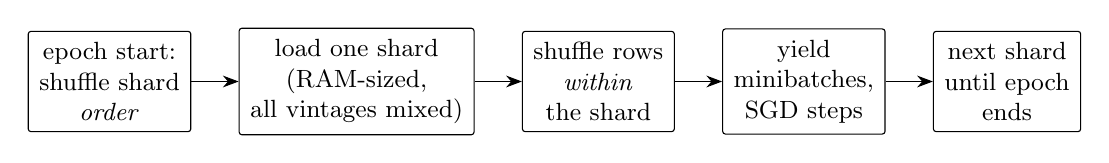
\begin{tikzpicture}[node distance=4mm and 6mm,
  box/.style={draw, rounded corners=1pt, align=center, font=\small, inner sep=4pt},
  arr/.style={-{Stealth[length=2mm]}}]
\node[box] (a) {epoch start:\\ shuffle shard\\ \emph{order}};
\node[box, right=of a] (b) {load one shard\\ (RAM-sized,\\ all vintages mixed)};
\node[box, right=of b] (c) {shuffle rows\\ \emph{within}\\ the shard};
\node[box, right=of c] (d) {yield\\ minibatches,\\ SGD steps};
\node[box, right=of d] (e) {next shard\\ until epoch\\ ends};
\draw[arr] (a) -- (b);
\draw[arr] (b) -- (c);
\draw[arr] (c) -- (d);
\draw[arr] (d) -- (e);
\end{tikzpicture}
\caption[The two-level shuffle over loan-keyed shards]{\textit{The
two-level shuffle.}  Random shard order across the epoch, full
shuffle within each RAM-sized shard.  Every minibatch mixes loans
from all vintages at streaming cost; a global shuffle of $10^9$ rows
is never performed.}
\label{fig:shardloop}
\end{figure}

Training then follows the two-level shuffle of
Figure~\ref{fig:shardloop}.  It is not exactly a uniform draw --- rows
in a batch share a shard --- but because each shard is already an
unbiased cross-section of loans, the residual within-shard
correlation is negligible for gradient quality.

\section{Covariates and feature construction}
\label{sec:meth-features}

Features comprise the loan-level fields and external macroeconomic
covariates described in Sections~\ref{sec:data-variables}
and~\ref{subsec:data-external}.  Continuous covariates are
standardised using moments estimated on each training window only
(Section~\ref{sec:meth-design}); heavily skewed balances enter in
logarithms.  High-cardinality categorical fields (property state,
metropolitan area, three-digit zip code) are mapped to learned dense
embedding vectors rather than one-hot columns, with categories unseen
in training routed to a reserved index.  Missingness indicators
accompany sentinel-scrubbed fields, since the fact of missingness is
itself predictive in credit data.

Two engineered covariates carry most of the economic content:
\begin{align}
\label{eq:incentive}
\text{(refinancing incentive)} \qquad
\mathrm{incentive}_{i,t} &= r^{\mathrm{cur}}_{i,t} - m(t),\\[2pt]
\label{eq:mtmltv}
\text{(mark-to-market LTV)} \qquad
\mathrm{ltv}^{\mathrm{mtm}}_{i,t} &=
\frac{\mathrm{UPB}_{i,t}}{\mathrm{UPB}_{i,0}}\;\cdot\;
\mathrm{LTV}_{i,0}\;\cdot\;
\frac{H_{s(i)}\!\left(t_0(i)\right)}{H_{s(i)}(t)},
\end{align}
where $m(t)$ is the prevailing 30-year mortgage rate,
$\mathrm{UPB}$ denotes the unpaid principal balance (so
$\mathrm{UPB}_t/\mathrm{UPB}_0$ is the fraction of the loan still
owed), and $H_s(\cdot)$ is the state-$s$ house-price index at the
indicated month.  Equation~\eqref{eq:incentive} measures how far the
borrower's refinancing option is in the money --- the dominant
prepayment driver \citep{schwartz1989} --- and
\eqref{eq:mtmltv} approximates the borrower's current leverage, the
key default driver \citep{deng2000}.  Raw calendar time is
deliberately excluded as a feature: test years are by construction
unseen, so a model leaning on ``year'' would extrapolate arbitrarily;
all time variation must flow through observable, recurring channels
(the macro block, seasonality encoded as month-of-year, and loan
age).

\section{Rolling out-of-sample design}
\label{sec:meth-design}

Credit models are used prospectively, so the evaluation is temporal:
train on the past, predict the future.  One subtlety deserves
emphasis because it is a one-character bug with real leakage
consequences: the label of the example built at feature month $t$ is
the state at $t{+}1$, so ``training on data up to month $T$'' must
mask on the \emph{label} month --- include the example only if
$t < T$ strictly, so that its label month $t{+}1 \le T$.

The primary design is a rolling, expanding-window backtest with one
window per test year $k = 2015,\dots,2025$:
\[
\underbrace{\text{train: labels} \le \mathrm{Dec}(k{-}2)}_{\text{expanding, starts 2000}}
\qquad
\underbrace{\text{validation: labels in year } k{-}1}_{\text{early stopping only}}
\qquad
\underbrace{\text{test: labels in year } k}_{\text{never touched in fitting}}
\]
Three rules keep this honest and affordable.  First,
\emph{tune once, freeze, roll}: architecture and regularisation
hyperparameters are selected once, on the $k{=}2015$ tuning window,
then frozen across all windows; per-window validation years serve
only early stopping.  Re-tuning every window would multiply compute
by the grid size and constitute a subtle multiple-testing problem.
Second, \emph{window-local preprocessing}: feature scalers, embedding
vocabularies, and any statistic estimated from data are re-fitted
within each window's training slice; standardising with full-sample
moments would leak future means and variances into the past.  Third,
\emph{pooled and per-year reporting}: each test row in 2015--2025 is
predicted exactly once, by a model that never saw it, and metrics are
reported per test year and pooled over all years.  Regime shifts ---
COVID in 2020--21, the rate shock of 2022--23 --- thus appear as
legible test-year effects rather than hinging on a single arbitrary
cutoff.

\paragraph{Class thinning with importance weights.}
\emph{Current}-to-\emph{Current} transitions are $96.3\%$ of
loan-months (Table~\ref{tab:stateshares}) and individually nearly
uninformative.  The training export therefore retains every row whose
origin or destination is not \emph{Current}, but keeps
\emph{Current}$\to$\emph{Current} rows only with probability $p$,
attaching weight $w_i = 1/p$ to kept rows ($w_i = 1$ otherwise).  The
training objective is the weighted negative log-likelihood
\begin{equation}
\label{eq:weightednll}
\widehat{\mathcal{L}}(\theta) \;=\;
\frac{1}{\sum_i w_i}\sum_{i \in \text{kept}} w_i\,
\bigl[-\log p_\theta\!\left(y_i \mid x_i\right)\bigr],
\end{equation}
a Horvitz--Thompson estimator of the full-sample loss
\citep{ht1952}: each row is kept with known probability and weighted
by its inverse, so the fitted model still estimates the \emph{true}
conditional probabilities --- unlike naive downsampling, which would
silently inflate every rare-event probability.  Validation and test
slices are never thinned, and a QA step compares ensemble-average
predicted base rates against unthinned panel frequencies.
Evaluation uses a fixed, loan-disjoint shard block ($\sim$20\% of
loans, the same loans in every window and for every model), so that
likelihood comparisons are exact rather than sampled apart.

\section{The model hierarchy}
\label{sec:meth-models}

The benchmarks are ordered by how flexibly they let
\eqref{eq:object} depend on covariates; each strictly nests or
dominates the previous, which is what makes the comparison
interpretable.

\subsection{Empirical transition matrix}
\label{subsec:meth-empirical}

The simplest estimator ignores covariates entirely: conditional only
on the origin state $u$, the destination distribution is estimated by
smoothed relative frequencies in the window's training slice,
\begin{equation}
\label{eq:empirical}
\widehat{P}_{uv} \;=\; \frac{N_{uv} + \alpha}{N_{u\cdot} +
\alpha\,|\mathcal{S}|}, \qquad \alpha = \tfrac12,
\end{equation}
where $N_{uv}$ counts $u\to v$ transitions.  The Laplace term
$\alpha$ guarantees no test transition receives probability zero (a
single unsmoothed empty cell would make the test log-likelihood
infinite).  This time-homogeneous Markov chain is the floor of the
comparison.  A ``bucketed'' variant conditioning additionally on
credit-score and incentive terciles shows how far cheap,
nonparametric conditioning goes before any model fitting.

\subsection{Multinomial logistic regression as a zero-layer network}
\label{subsec:meth-logit}

The workhorse of the empirical mortgage literature posits log-linear
odds:
\begin{equation}
\label{eq:logit}
p_\theta(j \mid x) \;=\; \operatorname{softmax}_j\!\left(Wx + b\right)
\;=\; \frac{\exp\!\left(w_j^\top x + b_j\right)}
{\sum_{j'} \exp\!\left(w_{j'}^\top x + b_{j'}\right)}.
\end{equation}
Crucially, \eqref{eq:logit} is exactly a neural network with zero
hidden layers, and it is implemented as such --- same data loader,
same loss \eqref{eq:weightednll}, same evaluation code as the deep
models, with a one-time numerical cross-check against a standard
library implementation.  This is an experimental-control choice: when
the deep network beats the logit, the difference is attributable to
architecture alone, not to differences in preprocessing, optimisation
or data.  An ``augmented'' logit with hand-crafted nonlinear terms
(squared loan age, splined incentive) quantifies how much of the gap
manual feature engineering can close.

\subsection{Deep neural networks}
\label{subsec:meth-nn}

The deep model composes $L$ hidden layers,
\begin{equation}
\label{eq:mlp}
z^{(0)} = \phi(x), \qquad
z^{(\ell)} = \sigma\!\left(W^{(\ell)} z^{(\ell-1)} + b^{(\ell)}\right),
\qquad
p_\theta(\cdot \mid x) =
\operatorname{softmax}\!\left(W^{(L+1)} z^{(L)} + b^{(L+1)}\right),
\end{equation}
with rectified-linear activations $\sigma(u)=\max(u,0)$ and the
input map $\phi$ of Section~\ref{sec:meth-features}.  Depth is
searched over $L\in\{1,3,5,7\}$ anchored at the five-layer geometry
preferred by \citet{sirignano2021} (200 units, then 140 per layer);
layer widths are inherited from that paper rather than searched ---
depth and regularisation are the first-order capacity knobs --- with
a half/paper/double width sweep at the selected configuration as a
completeness check (Appendix~\ref{app:supplementary}).  Each hidden
unit is a learned ``soft feature''; depth lets the network build
feature hierarchies, which is where interaction effects such as
incentive$\times$credit-score live --- the model discovers them
rather than being told.

Three regularisation devices mirror the paper: \emph{dropout}
\citep{dropout} on hidden layers (rates $\{0, 0.2, 0.5\}$), an
$\ell_2$ penalty ($\lambda \in \{0, 10^{-5}, 10^{-4}\}$), and
\emph{early stopping} on the window's validation likelihood --- the
only use the validation year is put to.  Finally, the headline model
is an \emph{ensemble}: $K{=}8$ independently initialised networks
trained on resampled shard subsets, with predicted probabilities
averaged, $\bar p(j\mid x) = \tfrac1K \sum_k p_{\theta_k}(j \mid x)$.
Averaging reduces the variance component of error from stochastic
training and finite data; the marginal value of each additional
member is traced in an ensemble-size curve.  Because eight fits per
window is the dominant compute cost, the ensemble runs on five
regime-spanning key windows ($k\in\{2015, 2019, 2020, 2023, 2025\}$),
with the single best network everywhere.

\section{Evaluation}
\label{sec:meth-eval}

The headline criterion is the out-of-sample mean negative
log-likelihood,
\begin{equation}
\label{eq:nll}
\mathrm{NLL} \;=\; -\frac{1}{N_{\mathrm{test}}}
\sum_{i\in\mathrm{test}} \log p_\theta\!\left(y_i \mid x_i\right),
\end{equation}
on identical, frozen, unthinned test rows for every model.  It is the
right primary metric for two reasons: it evaluates the full predicted
distribution over seven destinations rather than a binarised event,
and it is a strictly proper scoring rule --- uniquely minimised in
expectation by the true conditional probabilities, so a model cannot
improve it by distorting its probabilities.  Two complementary lenses
guard against failure modes a single number hides:
\emph{discrimination}, measured for each origin--destination pair by
the one-versus-rest area under the ROC curve (the probability that a
randomly chosen loan-month that truly makes the transition receives a
higher predicted probability than one that does not); and
\emph{calibration}, measured by reliability diagrams comparing
predicted probabilities to realised frequencies within prediction
buckets.  A model can rank well yet be systematically over- or
under-confident; calibration is what the pool-level counting of
Section~\ref{sec:meth-pool} actually consumes.

\section{From loans to pools}
\label{sec:meth-pool}

A mortgage pool's cashflow is the sum of its loans' events; a
mortgage-backed security (MBS) is priced off exactly such sums.
\citet{sirignano2021} argue the nonlinearity advantage
\emph{compounds} rather than washes out at the pool level, because
linear misspecification correlates across loans sharing
characteristics.

\subsection{Multi-month prediction by matrix composition}
\label{subsec:meth-rollforward}

The monthly model is rolled forward by composing transition
matrices.  For loan $i$ alive at anchor month $t_0$ with state
distribution $\rho_0$ (a one-hot vector), the model supplies for each
future month $h$ a $7\times 7$ matrix $P^{(i)}_h$ whose four
non-terminal rows are the model's predictions at the
deterministically evolved covariates and whose terminal rows are the
identity (absorbing states).  Then
\begin{equation}
\label{eq:rollforward}
\rho_h \;=\; \rho_0 \prod_{h'=1}^{h} P^{(i)}_{h'},
\qquad
\mathbb{P}\!\left(\text{loan } i \text{ prepaid by } t_0{+}H\right)
= \left[\rho_H\right]_{\mathrm{Prepaid}},
\end{equation}
with horizon $H=12$ months.  Because terminal states are absorbing
and the full state distribution is tracked,
\eqref{eq:rollforward} is exact under the model --- no Monte Carlo
simulation is required.  Covariates evolve deterministically (age and
remaining term advance, seasonality follows the calendar) while
balances and the macroeconomic block are frozen at $t_0$: predictions
are explicitly \emph{conditional on the anchor-date environment}.
For ``ever reaches 60+ days past due within the horizon'' a
first-passage construction is used: delinquency states can be entered
and cured out of, so month-$H$ occupancy undercounts loans that
visited and recovered; making the target set absorbing in a modified
chain yields the probability of ever hitting it.

\subsection{Pools and pool-level prediction}
\label{subsec:meth-pools}

Pools are formed two ways at each window anchor: characteristic
buckets (credit score $\times$ original rate $\times$
loan-to-value cells, the criteria a securitisation structurer would
use) and random pools ($B$ pools of $N$ loans), which give a
bucketing-free comparison.  With per-loan horizon probabilities $q_i$
from \eqref{eq:rollforward}, the predicted event count in pool
$\mathcal{P}$ and its approximate distribution are
\begin{equation}
\label{eq:poolcount}
\widehat{C}_{\mathcal{P}} = \sum_{i\in\mathcal{P}} q_i,
\qquad
C_{\mathcal{P}} \;\dot\sim\;
\mathcal{N}\!\Bigl(\textstyle\sum_i q_i,\; \sum_i q_i(1-q_i)\Bigr),
\end{equation}
the Gaussian being the standard approximation to the
Poisson--binomial distribution of a sum of independent non-identical
Bernoulli variables (conditional independence given covariates is the
maintained assumption, inherited from the paper).  Models are
compared on predicted versus realised counts, with interval coverage
testing the distributional claim in \eqref{eq:poolcount}, not just
its mean.

\subsection{Economic translation: prepayment speed, cashflow timing, and price}
\label{subsec:meth-econ}

The final step converts counts into valuation units; each term is
defined as it first appears.  Averaging the loans' monthly prepayment
probabilities with each loan weighted by its unpaid principal balance
gives the pool's \textbf{prepayment-speed path}: the model's
month-by-month forecast of what fraction of the pool's remaining
principal prepays --- the units and weighting that pool cashflows
actually obey, since a large loan returns proportionally more
principal than a small one.  (Market shorthand, used hereafter: the
monthly fraction is the \emph{single monthly mortality}, SMM;
annualised it is the \emph{conditional prepayment rate}, CPR.)  The
realised path is computed identically from the panel.  A
deterministic cashflow engine turns any speed path into pool
cashflows, treating the pool as a \emph{pass-through} (investors
receive the pool's interest and principal as it is paid): scheduled
amortisation plus forecast prepayments, month by month, with the
final month's speed held constant beyond the horizon.  From the
cashflows follow two valuation summaries: \textbf{weighted-average
life} --- the average time a dollar of principal remains outstanding,
i.e.\ the timing of money returned --- and \textbf{price}, the
discounted value of the cashflows, with every model's cashflows
discounted at the same fixed rate so that any price difference comes
from the prepayment forecasts alone.  The comparison metrics are then
a speed error (percentage points of CPR), a timing error (months of
weighted-average life), and a price error (per 100 of face value),
per pool, model, and anchor.  The engine is unit-tested against two
closed forms (with no prepayment a pool is a textbook annuity; a
constant speed has a closed-form survival schedule).  With the
macroeconomic environment frozen at the anchor and a common fixed
discount rate, the exercise isolates the \emph{prepayment-model
component} of valuation error --- deliberately simpler than the
market's full option-adjusted-spread machinery.

\paragraph{Why pricing rather than portfolio sorts.}
\citet{sirignano2021} demonstrate economic significance with a
portfolio-sort exercise: rank pools by predicted prepayment risk,
form best- and worst-decile portfolios, and compare their realised
outcomes.  This study runs the pricing exercise instead, and the
choice deserves a plain explanation.  The two designs test different
properties of the same predictions.  A sort uses only the
\emph{ordering} of pools --- it is blind to probability levels, so a
model whose hazards are uniformly twice the truth sorts exactly as
well as a perfectly calibrated one.  Pricing uses the \emph{levels}:
weighted-average life and price depend on the actual magnitude of the
predicted prepayment path.  Ranking-only evidence is the natural
choice where levels are inherently untrustworthy (the classic
asset-pricing setting); here, by contrast, the transition
probabilities are explicitly calibration-checked
(Section~\ref{sec:meth-eval}), so a ranking-only exercise would
discard the model's strongest property --- and the practical consumer
of a pool-level mortgage model (pricing a pool, marking it to market,
hedging a position in it) consumes levels, not ranks.  Running both
would add little: each is a deterministic re-presentation of the same
per-loan probabilities, their respective properties are already
tested more rigorously upstream (discrimination by the AUC tables,
calibration by the reliability diagrams), and the bucket-level
price-error map conveys what a sort would dramatise --- \emph{where}
the linear model goes wrong --- while also conveying by \emph{how
much}, in the units the market trades.  The sort exercise is
therefore noted as future work rather than duplicated.

\section{Reproducibility}
\label{sec:meth-repro}

Every model fit writes a self-describing run record (configuration,
code version, data-manifest hash, window identity, metrics), so any
number reported in Chapter~\ref{chap:results} can be traced to the
exact code and data slice that produced it.  Correctness-critical
components carry unit tests: the leakage mask, the importance
weights, the mark-to-market LTV construction, the roll-forward engine
against a closed-form chain, and the cashflow engine against the
annuity closed forms.  Appendix~\ref{app:reproducibility} records the
computing environment and data snapshot conventions.
          % Methodology
% ============================================================
%  Chapter 3 — Data
%  Drop this file into your dissertation root and add
%      % ============================================================
%  Chapter 3 — Data
%  Drop this file into your dissertation root and add
%      % ============================================================
%  Chapter 3 — Data
%  Drop this file into your dissertation root and add
%      \include{chapter3}
%  to main.tex (after chapter2, before conclusions).
%
%  Required packages (add to the preamble of main.tex):
%      \usepackage{booktabs}
%      \usepackage{tabularx}
%      \usepackage{multirow}
%      \usepackage{natbib}   % or your preferred bib style
% ============================================================

\chapter{Data}
\label{chap:data}

% ────────────────────────────────────────────────────────────
\section{Data Source}
\label{sec:data-source}

This study employs the Fannie Mae Single-Family Loan Performance
(SFLP) dataset, a publicly available research dataset maintained by
the Federal National Mortgage Association (Fannie Mae) and updated on
a quarterly basis.  The dataset was originally released in April 2013
and contains origination and monthly performance records for a subset
of single-family conventional mortgage loans acquired by Fannie Mae
since January 2000.  New loan acquisitions and performance data are
added with an approximate four-month lag following the end of each
calendar quarter \citep{fanniemae2024}.

The data are organised as a \emph{loan-month panel}: each observation
corresponds to a single mortgage loan in a single monthly reporting
period, beginning at the month of acquisition and continuing until the
loan terminates through full prepayment, foreclosure, Real Estate
Owned (REO) disposition, or contractual maturity, or until the data
cut-off date.  This longitudinal structure is well-suited to the
competing-risks framing of \citet{sirignano2021}, which the present
study adapts to the Fannie Mae data.

Raw files are distributed as pipe-delimited CSV without a header row,
organised by acquisition quarter and identified by the convention
\texttt{YYYYQn.csv}.  Column identities are positional, fully
specified in the Fannie Mae Single-Family Loan Performance Data File
Layout and Glossary.  Each row contains 113 fields encoding static
origination attributes, dynamic monthly performance measures, and
post-termination expense and proceeds data.  The estimation sample
employed in this study is the \emph{complete} vintage set from a
single quarterly release: 104 acquisition-quarter files covering
cohorts from 2000Q1 onwards, with monthly reporting periods from
January 2000 through December 2025.  The assembled panel comprises
\textbf{3{,}312{,}456{,}883 loan-month observations across
57{,}562{,}668 loans} --- performance histories spanning four
interest-rate cycles, the 2008--11 foreclosure crisis, the COVID-era
forbearance episode, and the 2022--23 rate shock.

\subsection{From raw files to the estimation panel}
\label{subsec:data-pipeline}

Three distinct concepts in this dataset are colloquially called a
``quarter,'' and distinguishing them prevents the most common
assembly errors.  The \emph{acquisition vintage} identifies a file:
each \texttt{YYYYQn.csv} contains the loans Fannie Mae acquired in
that quarter, carrying their entire subsequent monthly history, and a
loan appears in exactly one file --- so concatenating all files
assembles the full sample with no duplication.  The \emph{monthly
reporting period} identifies a row, and this time dimension --- not
redundancy --- is why the dataset is large.  The \emph{release}
identifies the download: Fannie Mae republishes the entire dataset
quarterly with extended histories, so all files must come from one
release lest vintages carry inconsistent right-censoring dates; an
ingestion audit verifies a uniform cut-off across all 104 files.

Because no single file fits in memory ($\sim$800\,GB of raw CSV in
total), a six-stage pipeline converts the files into a compressed,
columnar store queried out of core: an integrity audit, streaming
conversion, type and sentinel cleaning, construction of the
transition panel with the outcome variable of
Section~\ref{sec:data-outcome}, sampling utilities, and a
reconciliation step that verifies row counts against the raw files.
Columnar storage means a query touching six of the 113 fields reads
roughly five per cent of the bytes, which is what makes the
full-panel descriptive statistics and exploratory analysis of
Sections~\ref{sec:data-summary} and~\ref{sec:data-eda}
computationally cheap.

% ────────────────────────────────────────────────────────────
\section{Population and Eligibility}
\label{sec:data-population}

The primary dataset is not a census of all loans in Fannie Mae's
guarantee book; it is a curated research sample subject to documented
eligibility and exclusion criteria \citep{fanniemae2024}.  The
population is restricted to fixed-rate, fully amortising,
full-documentation single-family conventional mortgage loans with
original terms of at least five years and less than 35 years,
originated on or after 1 January 1999 and acquired by Fannie Mae on
or after 1 January 2000.

A number of product types are explicitly excluded.  Adjustable-rate
mortgages, interest-only loans, balloon-amortisation mortgages, and
loans carrying prepayment penalties are absent from the dataset.
Also excluded are loans with original loan-to-value (LTV) ratios
exceeding 97 per cent, Alt-A and other reduced-documentation
products, government-insured loans (FHA and VA), loans subject to
long-term standby commitments or third-party risk-sharing
arrangements other than primary mortgage insurance, and loans
acquired on a negotiated bulk basis.  Loans with non-standard payment
due dates and loans that liquidated in the same month as acquisition
are similarly excluded.  Fannie Mae's Home Affordable Refinance
Program (HARP) loans are likewise absent from the primary dataset;
when a loan in the primary dataset was subsequently refinanced through
HARP, its termination is recorded as a standard prepayment, and its
post-refinance performance is not tracked here.  This is discussed
further in Section~\ref{sec:data-outcome}.

These restrictions yield a sample of conventionally underwritten
fixed-rate mortgages broadly representative of the agency conventional
loan market under post-crisis underwriting standards.  The exclusion
of adjustable-rate and interest-only products limits the range of
prepayment incentive dynamics captured relative to the full-spectrum
dataset used by \citet{sirignano2021}; this is discussed in
Section~\ref{sec:data-comparison}.  Table~\ref{tab:eligibility}
summarises the principal eligibility criteria and exclusions.

\begin{table}[htbp]
  \centering
  \small
  \begin{tabularx}{\textwidth}{@{} l X @{}}
    \toprule
    \textbf{Criterion} & \textbf{Requirement / Exclusion} \\
    \midrule
    Origination date      & On or after 1 January 1999 \\[2pt]
    Acquisition date      & On or after 1 January 2000 \\[2pt]
    Product type          & Fixed-rate, fully amortising only \\[2pt]
    Loan term             & $5 \leq \mathrm{term} < 35$ years at origination \\[2pt]
    Documentation         & Full documentation only \\[2pt]
    LTV at origination    & $\leq 97\%$ \\[4pt]
    \emph{Excluded: product}      & ARM, interest-only, balloon,
                                    prepayment-penalty loans \\[2pt]
    \emph{Excluded: credit class} & Alt-A, reduced-documentation,
                                    streamlined processing \\[2pt]
    \emph{Excluded: guarantee}    & Government-insured (FHA, VA) loans \\[2pt]
    \emph{Excluded: structure}    & Long-term standby commitments;
                                    bulk acquisitions; lender-recourse
                                    loans (except primary MI) \\[2pt]
    \emph{Excluded: programme}    & HARP and Refi Plus loans \\[2pt]
    \emph{Excluded: payment}      & Bi-weekly and non-first-of-month
                                    due dates \\[2pt]
    \emph{Excluded: timing}       & Loans liquidated in month of
                                    acquisition \\
    \bottomrule
  \end{tabularx}
  \caption[Eligibility criteria for the Fannie Mae SFLP primary dataset]%
  {\textit{Eligibility criteria for the Fannie Mae SFLP primary
  dataset.}  Source: Fannie Mae Single-Family Loan Performance
  Dataset FAQs \citep{fanniemae2024}.}
  \label{tab:eligibility}
\end{table}

% ────────────────────────────────────────────────────────────
\section{Variables}
\label{sec:data-variables}

The 113 fields in each monthly observation can be organised into three
functional groups: static origination attributes, dynamic monthly
performance attributes, and post-termination resolution data.  The
model uses a subset of these fields as covariates.  Two fields --- the
Current Loan Delinquency Status and the Zero Balance Code --- serve as
the primary inputs from which the outcome variable is constructed.

% ────────────────────────────────
\subsection{Origination Attributes}
\label{subsec:data-origination}

Static origination attributes are recorded at loan delivery and do
not change over the life of the loan absent a modification.  The
borrower's FICO credit score at origination is available for both the
primary borrower and, where applicable, a co-borrower; prior to the
January 2015 dataset release only the lower of the two scores was
disclosed, and a missingness indicator is constructed accordingly.
Continuous origination covariates include the original
debt-to-income (DTI) ratio, original LTV ratio, original combined LTV
(CLTV, which incorporates subordinate liens), original unpaid
principal balance (UPB), original interest rate, and original loan
term in months.  Categorical origination attributes include the
acquisition channel (retail, broker, or correspondent), loan purpose
(purchase, rate-term refinance, or cash-out refinance), property type,
occupancy status (primary residence, second home, or investment
property), property state, Metropolitan Statistical Area (MSA), and
three-digit truncated zip code.  The truncation of the zip code
reflects borrower privacy considerations; full zip codes are not
disclosed in the dataset \citep{fanniemae2024}.

% ────────────────────────────────
\subsection{Dynamic Performance Attributes}
\label{subsec:data-performance}

Dynamic performance attributes are updated in each monthly reporting
period.  The current actual unpaid principal balance reflects the
outstanding loan balance at each point in time.  Loan age, measured
in months from the first payment date, and the remaining months to
legal maturity are derived from the contractual amortisation schedule.
The current interest rate reflects the applicable note rate, updated
when a modification changes the loan terms.

Two dynamic fields jointly determine the outcome variable.  The
\textbf{Current Loan Delinquency Status} reports the number of missed
monthly payments as a two-character code: \texttt{00} denotes a
current loan; \texttt{01}, \texttt{02}, and codes \texttt{03} and
above denote 30-, 60-, and 90-or-more-day delinquencies respectively;
and \texttt{XX} denotes an unavailable status.  The \textbf{Zero
Balance Code} is populated exclusively in the terminal monthly
observation and classifies the manner of loan termination into nine
categories, distinguishing between voluntary prepayments, third-party
foreclosure sales, short sales, repurchases, REO dispositions, note
sales, and non-credit removals.  (The dataset also carries a 24-month
payment-history string; it is not used as a model input here, since
the current state and loan-level covariates already summarise the
information the transition model conditions on.)

% ────────────────────────────────
\subsection{Externally Sourced Covariates}
\label{subsec:data-external}

A small, fixed set of external macroeconomic series is joined to the
loan-level panel at feature-construction time (the stored panel
itself is never rewritten); Table~\ref{tab:macrovars} summarises the
sources.  The Freddie Mac Primary Mortgage Market Survey (PMMS)
weekly fixed-rate series, aggregated to calendar-month means, supplies
the prevailing market mortgage rate from which the \emph{rate
incentive} of Equation~\eqref{eq:incentive} is computed --- the
refinancing option value, the primary driver of prepayment behaviour
in the empirical mortgage literature
\citep{schwartz1989,sirignano2021}.  Unemployment rates enter at both
national (Bureau of Labor Statistics) and state level, the latter
because the cross-sectional dispersion in labour-market conditions
(Nevada versus Texas in 2009) is precisely the variation a national
series cannot supply.  House prices enter through the Freddie Mac
House Price Index at national and state level, from which the
mark-to-market loan-to-value ratio of Equation~\eqref{eq:mtmltv} ---
the principal determinant of the default option value
\citep{deng2000} --- and the trailing twelve-month house-price change
are constructed.  The ten-year Treasury yield completes the set.

Each series is joined with a \emph{publication lag} reflecting when
the value was actually observable: rates are published in real time
(no lag), month-$t$ unemployment is released early in month $t{+}1$
(one-month lag), and the house-price index roughly two months after
the reference month (two-month lag).  Final-revision series are used
rather than real-time vintages --- a stated limitation, standard for
historical studies.  Where a state-level value is unavailable
(territories; series start dates) the national value substitutes,
with an indicator flag carried as a model feature.

\begin{table}[htbp]
  \centering
  \small
  \begin{tabularx}{\textwidth}{@{} l l l l c @{}}
    \toprule
    \textbf{Variable} & \textbf{Source} & \textbf{Geography}
      & \textbf{Monthly value} & \textbf{Lag} \\
    \midrule
    30-yr mortgage rate & Freddie Mac PMMS & national & month mean & 0\,m \\
    10-yr Treasury yield & FRED \texttt{DGS10} & national & month mean & 0\,m \\
    Unemployment rate & BLS (via FRED) & national + state & as published & 1\,m \\
    House-price index & Freddie Mac FMHPI & national + state & as published & 2\,m \\
    \bottomrule
  \end{tabularx}
  \caption[External macroeconomic covariates and join conventions]%
  {\textit{External macroeconomic covariates and join conventions.}
  A loan-month at calendar month $t$ is joined to the macro value of
  month $t-\ell$, where $\ell$ is the publication lag.  Seasonally
  adjusted versions are used throughout.}
  \label{tab:macrovars}
\end{table}

As a check on the incentive variable, a market-rate proxy derived
from the panel itself --- the average note rate of loans originated
in each calendar month --- tracks the PMMS series with correlation
$0.991$, root-mean-square deviation $0.198$ percentage points, and
mean absolute deviation $0.147$ percentage points, with a mean gap of
essentially zero.  The PMMS-based incentive is the primary feature;
the panel-derived proxy is retained as a robustness alternative,
demonstrating that the incentive variable is not an artefact of one
data source.

% ────────────────────────────────────────────────────────────
\section{Outcome Variable}
\label{sec:data-outcome}

Following \citet{sirignano2021}, the outcome variable is a categorical
measure of mortgage state in month $t+1$, conditional on the loan's
state and covariate vector in month $t$.  Seven mutually exclusive
states are defined: \emph{Current}, \emph{30 Days Past Due}
(30\,DPD), \emph{60 Days Past Due} (60\,DPD), \emph{90+ Days Past
Due} (90+\,DPD), \emph{Foreclosure}, \emph{Real Estate Owned} (REO),
and \emph{Prepaid}.

State assignment for each loan-month observation follows a
deterministic hierarchy.  When the Zero Balance Code is present ---
indicating the terminal observation for the loan --- the termination
type is mapped to the Foreclosure, REO, or Prepaid absorbing state as
shown in Table~\ref{tab:state-mapping}.  When the Zero Balance Code is
absent, the delinquency status field governs: codes \texttt{00}
through \texttt{03} and above map to Current, 30\,DPD, 60\,DPD, and
90+\,DPD respectively, while \texttt{XX} is treated as missing.  The
state in month $t+1$ is obtained by a window lead over the reporting
period dimension, partitioned by loan identifier.  Loans whose final
observation falls at or before the data cut-off without a recorded
termination event receive a censored indicator and are excluded from
the labelled target.

Regarding HARP loans: as noted in Section~\ref{sec:data-population},
any loan in the primary dataset that was refinanced through the
HARP programme terminates with a Zero Balance Code of \texttt{01}
(prepaid) at the moment of refinancing and is therefore treated as a
standard prepayment in the outcome variable.  This approximation is
defensible given that the loan is extinguished from Fannie Mae's
credit exposure in either case, though it may marginally overstate
the rate-incentive sensitivity of the prepayment hazard during the
period of peak HARP activity (approximately 2009--2013).

\begin{table}[htbp]
  \centering
  \small
  \begin{tabularx}{\textwidth}{@{} l l l X @{}}
    \toprule
    \textbf{State} & \textbf{Source field} & \textbf{Condition}
      & \textbf{Economic interpretation} \\
    \midrule
    Current
      & Delinquency Status & \texttt{= 00}
      & Borrower is contractually current on all payments. \\[3pt]
    30\,DPD
      & Delinquency Status & \texttt{= 01}
      & One missed monthly payment. \\[3pt]
    60\,DPD
      & Delinquency Status & \texttt{= 02}
      & Two consecutive missed monthly payments. \\[3pt]
    90+\,DPD
      & Delinquency Status & \texttt{$\geq$ 03}
      & Three or more missed payments; serious delinquency. \\[3pt]
    Foreclosure
      & Zero Balance Code  & \texttt{02, 03, 15,}
      & Credit-loss termination: third-party sale, short sale, \\
      &                    & \texttt{97, 98}
      & note sale, or credit-event repurchase. \\[3pt]
    REO
      & Zero Balance Code  & \texttt{= 09}
      & Fannie Mae acquires ownership of the property. \\[3pt]
    Prepaid
      & Zero Balance Code  & \texttt{01, 06, 16,}
      & Full payoff, contractual maturity, repurchase, \\
      &                    & \texttt{96}
      & or non-credit removal (including HARP exits). \\
    \bottomrule
  \end{tabularx}
  \caption[Mapping of Fannie Mae data fields to the seven-state
  outcome variable]%
  {\textit{Mapping of Fannie Mae data fields to the seven-state
  outcome variable.}  The Zero Balance Code is populated only in the
  terminal monthly observation; the Delinquency Status governs state
  assignment in all non-terminal periods.}
  \label{tab:state-mapping}
\end{table}

One structural feature of this dataset deserves emphasis: because the
Foreclosure, REO, and Prepaid states are derived from the Zero
Balance Code --- populated only in a loan's final observation ---
these three states are \emph{absorbing}.  There is no ongoing ``in
foreclosure'' monthly status as in the CoreLogic data of
\citet{sirignano2021}, where loans in formal foreclosure are observed
month by month and occasionally return to performing status.  The
origin set here therefore comprises the four live states (Current
through 90+\,DPD) while destinations span all seven: the transition
matrix is $4\times 7$ rather than $7\times 7$
(Section~\ref{sec:meth-model}).  Within the live states the data are
rich in both directions --- delinquency deepens at most one bucket
per month, but cures can jump multiple buckets, and a meaningful
fraction of seriously delinquent loans return to current.  The
seven-state formulation captures this in a way that a binary
default-versus-prepayment classification would obscure, and the
empirical monthly transition matrix derived from each training window
serves as the floor benchmark for the model comparison
(Section~\ref{subsec:meth-empirical}).

% ────────────────────────────────────────────────────────────
\section{Panel Composition and Summary Statistics}
\label{sec:data-summary}

The assembled panel comprises 3{,}312{,}456{,}883 loan-month
observations across 57{,}562{,}668 loans in 104 acquisition-vintage
partitions, with reporting months from January 2000 through December
2025.  Table~\ref{tab:stateshares} reports the distribution of
loan-months across the seven states.  Two features dominate.  First,
extreme class imbalance: the Current state accounts for $96.28\%$ of
all loan-months, while the credit-event terminals occur at roughly
one in ten thousand observations --- the empirical fact behind both
the importance-weighted thinning of training data
(Section~\ref{sec:meth-design}) and the Laplace smoothing of the
empirical benchmark (Section~\ref{subsec:meth-empirical}).  Second,
the rare states are nonetheless abundantly populated in absolute
terms (REO alone contributes roughly half a million loan-months),
which is what permits stable estimation of rare-transition
probabilities at this scale.

\begin{table}[htbp]
  \centering
  \small
  \begin{tabular}{l r @{\qquad\qquad} l r}
    \toprule
    \textbf{State} & \textbf{Share} & \textbf{State} & \textbf{Share} \\
    \midrule
    Current  & 96.28\,\% & 60\,DPD     & 0.31\,\%   \\
    Prepaid  & 1.25\,\%  & REO         & 0.014\,\%  \\
    30\,DPD  & 1.15\,\%  & Foreclosure & 0.0067\,\% \\
    90+\,DPD & 0.98\,\%  &             &            \\
    \bottomrule
  \end{tabular}
  \caption[Distribution of loan-months across the seven states]%
  {\textit{Distribution of loan-months across the seven states},
  full panel, 2000--2025 (3.31 billion loan-months).}
  \label{tab:stateshares}
\end{table}

Pooled over time, the monthly transition rates out of Current are
$1.27\%$ to Prepaid and $0.64\%$ to 30\,DPD.  The pooling, however,
hides the economics: Figure~\ref{fig:transitionrates} plots the
monthly series over 2000--2025, displaying the 2003 and 2020--21
refinancing waves in the prepayment rate, the 2008--11 default wave
in the delinquency rates, and the sharp 2022--23 collapse in
prepayments as market rates rose.  These regime shifts --- rather
than any single structural break --- are the empirical justification
for the rolling backtest design of Section~\ref{sec:meth-design}.
During 2020--21 the delinquency-status codes additionally reflect
COVID-era forbearance, which manifests as unusual persistence in
delinquency states followed by elevated cure rates; no special
treatment is applied, but results involving those years are read with
this in mind.

\begin{figure}[htbp]\centering
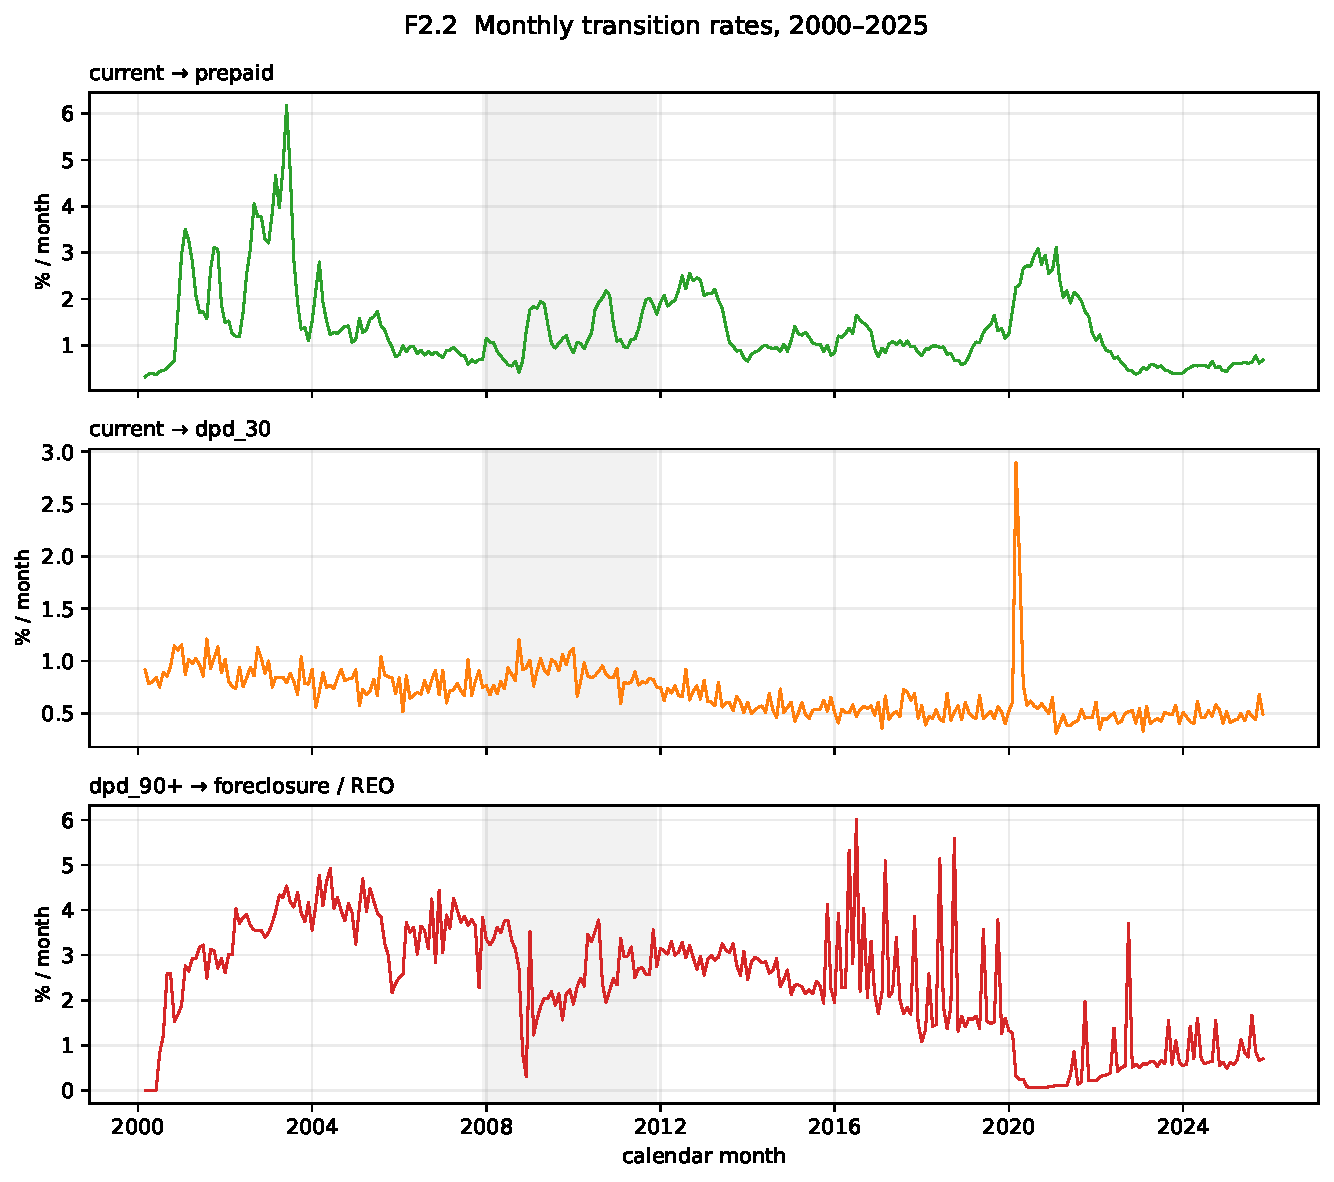
\includegraphics[width=0.9\textwidth]{figs/F2.2_transition_rates.pdf}
\caption[Monthly transition rates out of the Current state]{Monthly
transition rates out of the Current state, 2000--2025: prepayment and
entry into 30\,DPD (left axis), serious-delinquency terminations
(right axis).  Vertical shading marks the 2008--11 crisis and the
2020--21 forbearance episode.}\label{fig:transitionrates}
\end{figure}

\begin{table}[htbp]\centering\small
\caption[Summary statistics of model covariates]{Summary statistics of
the continuous model covariates over the full panel: null rate, mean,
standard deviation, and the min/1st/25th/50th/75th/99th/max
percentiles.}\label{tab:covariate-summary}
\resizebox{\textwidth}{!}{\input{figs/T1.2_covariate_summary.tex}}
\end{table}

% ────────────────────────────────────────────────────────────
\section{Exploratory Evidence: Nonlinearity and Interactions}
\label{sec:data-eda}

Before any model is fitted, the case that nonlinear modelling is
\emph{needed} can be made by counting alone.  The instrument is the
empirical hazard curve: bucket a covariate into equal-population
bins and plot the realised one-month transition rate per bin, with
Wilson 95\% confidence intervals.  Because each curve is a single
out-of-core aggregation over the columnar panel, the entire
programme runs in minutes.

\subsection{Single-covariate nonlinearity}
\label{subsec:data-eda-single}

Three hazard curves carry the argument.
\emph{Prepayment versus loan age}
(Figure~\ref{fig:hazard-age}): the rate rises from $0.27\%$ per month
at origination to a peak of $1.56\%$ at approximately 17 months of
age, then decays to $1.11\%$ by month 52 --- the classic
``seasoning hump,'' strongly non-monotone, with a secondary late-life
rise among long-surviving loans.  \emph{Prepayment versus the
refinancing incentive} (Figure~\ref{fig:hazard-incentive}): the rate
is flat at $0.4$--$0.6\%$ per month while the option is out of the
money, turns up sharply through zero, peaks at $2.71\%$ near
$+1.5$ percentage points of incentive, and falls back to $2.16\%$ by
$+2.7$ --- a roughly sevenfold range containing both an inflection
and a turning point, reproducing the flagship nonlinearity of
\citet{sirignano2021} on this cleaner credit box.
\emph{Delinquency versus credit score}
(Figure~\ref{fig:hazard-fico}): the entry rate into 30\,DPD falls
twenty-four-fold, from $3.06\%$ per month at FICO ${\approx}623$ to
$0.13\%$ at FICO ${\approx}815$, and the decay is convex --- the
slope in the low-score half is roughly $3.7$ times that in the
high-score half.  None of the three shapes is representable by a
linear term.

\begin{figure}[htbp]\centering
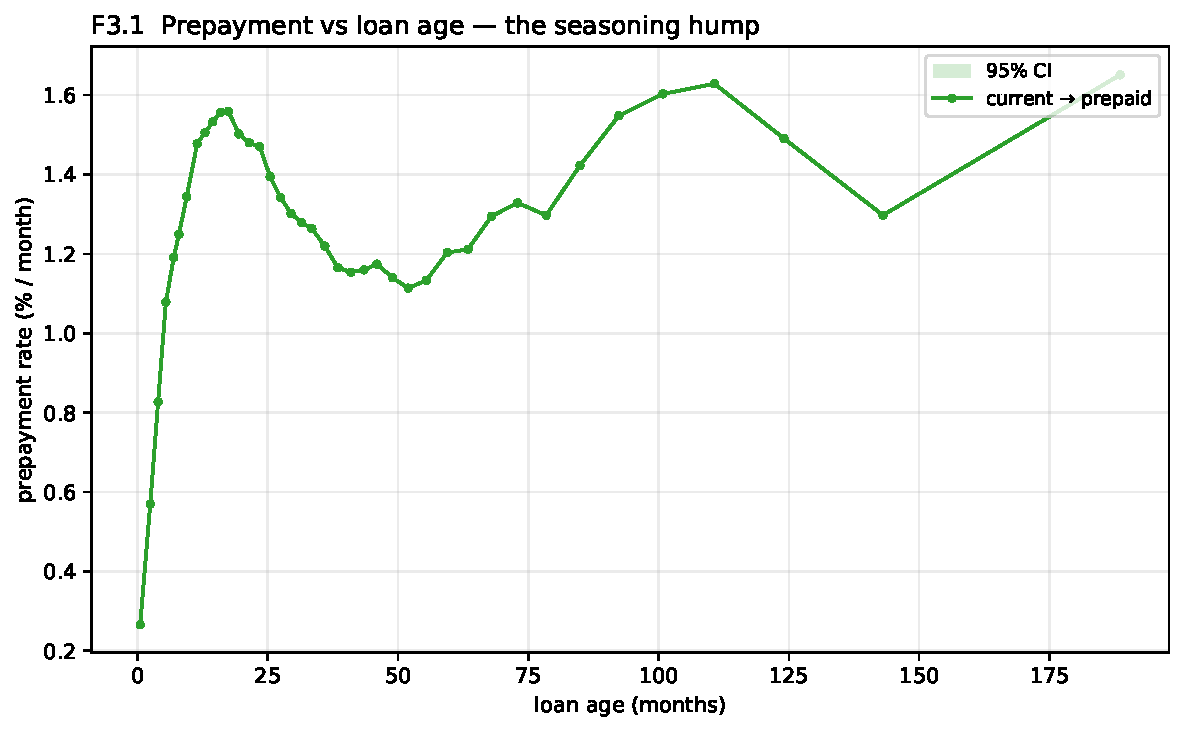
\includegraphics[width=0.8\textwidth]{figs/F3.1_prepay_age.pdf}
\caption[Empirical prepayment hazard by loan age]{Empirical prepayment
hazard by loan age (equal-population buckets, Wilson 95\% intervals):
the seasoning hump.}\label{fig:hazard-age}
\end{figure}

\begin{figure}[htbp]\centering
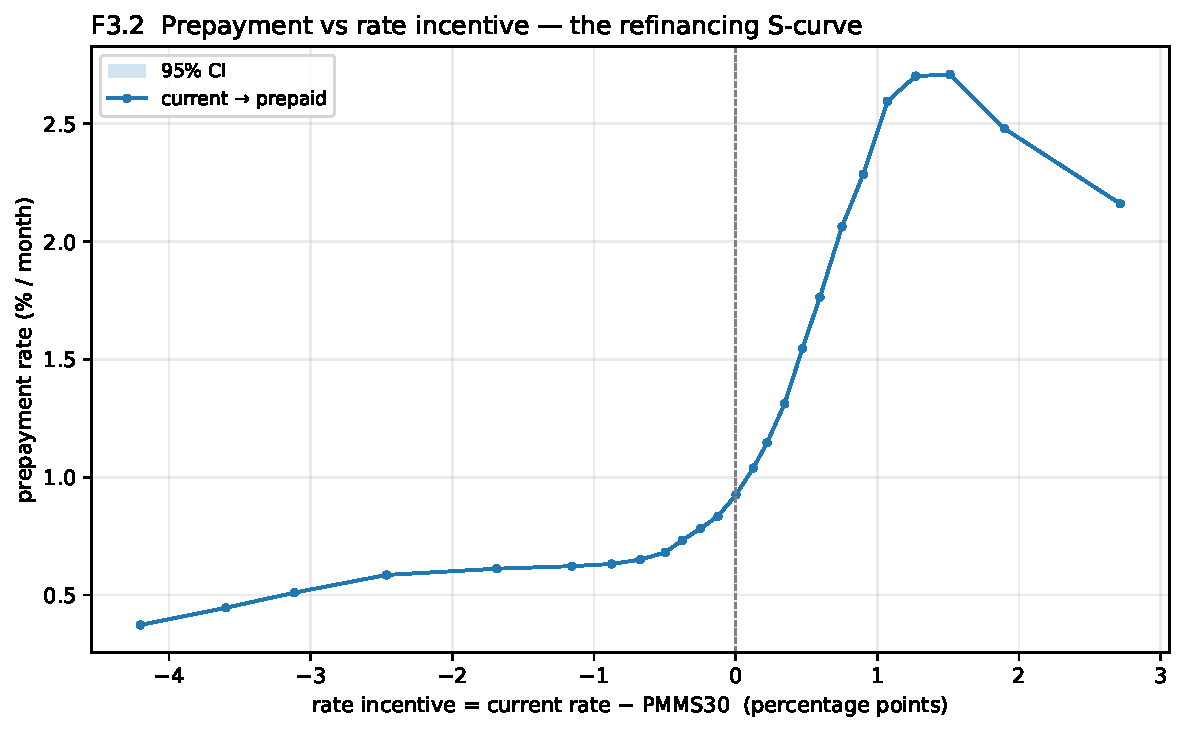
\includegraphics[width=0.8\textwidth]{figs/F3.2_prepay_incentive.pdf}
\caption[Empirical prepayment hazard by refinancing incentive]{Empirical
prepayment hazard by refinancing incentive: the S-curve, with burnout
beyond $+1.5$\,pp.}\label{fig:hazard-incentive}
\end{figure}

\begin{figure}[htbp]\centering
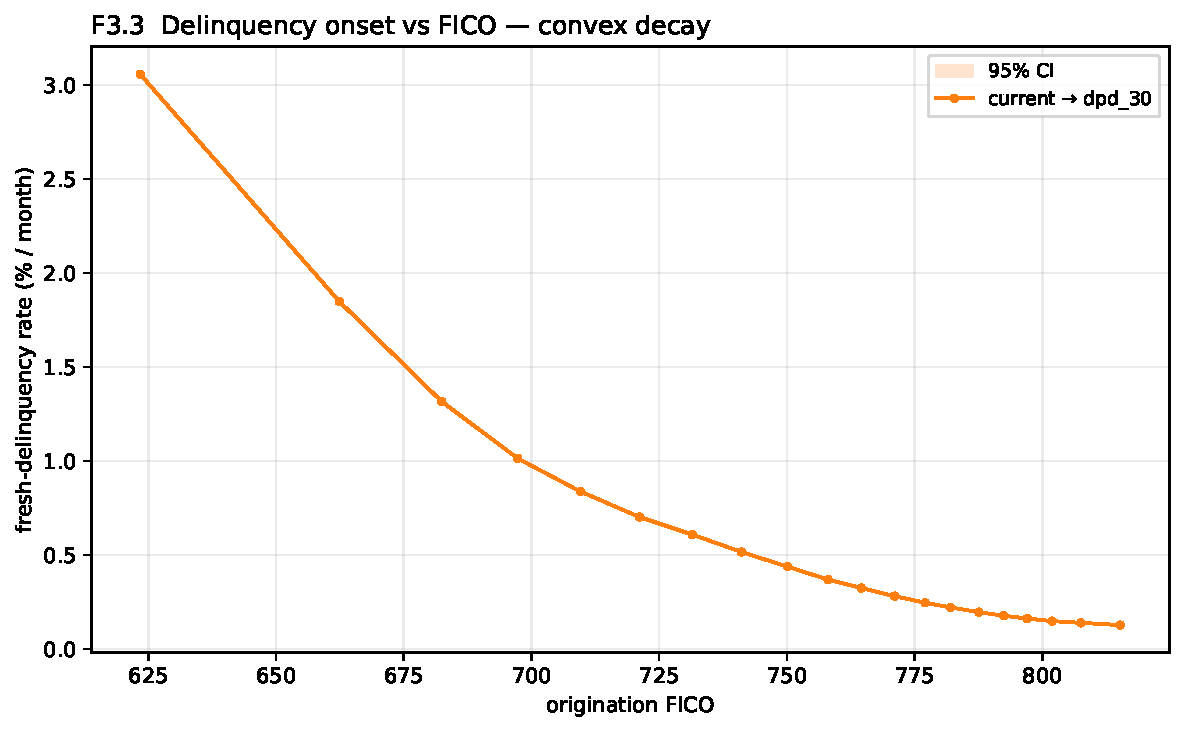
\includegraphics[width=0.8\textwidth]{figs/F3.3_delinq_fico.pdf}
\caption[Empirical 30\,DPD entry hazard by origination credit
score]{Empirical 30\,DPD entry hazard by origination credit score:
convex decay.}\label{fig:hazard-fico}
\end{figure}

\subsection{Interactions: the case against additivity}
\label{subsec:data-eda-interactions}

A linear-\emph{additive} model could in principle be patched with
transformed single-variable terms; interactions are what it cannot
absorb.  On a credit-score~$\times$~LTV grid
(Figure~\ref{fig:interaction-ficoltv}), the monthly rate of entry
into delinquency ranges from $0.11\%$ (best scores, lowest leverage)
to $2.69\%$ (worst scores, highest leverage) --- and decisively, the
\emph{additive} credit-score gradient (worst-minus-best rate) grows
from $1.73$ percentage points at low LTV to $2.48$ at high LTV, a
$43\%$ increase; equivalently, the leverage effect is roughly
$8.5$ times larger for low-score than high-score borrowers.
Additivity forces this gradient to be constant; the violation sits
exactly in the low-score/high-leverage corner that drives credit
losses.  In the prepayment channel
(Figure~\ref{fig:interaction-incfico}), splitting the incentive
S-curve by credit-score tercile shows the in-the-money refinancing
response \emph{rising} with credit quality --- $2.36\%$ per month in
the lowest tercile against $3.01\%$ in the highest --- because
credit-constrained borrowers cannot exercise the option: the
incentive \emph{slope} itself depends on the score.  Finally, holding
loan age fixed at 12--36 months to strip out seasoning, the
delinquency hazard by origination cohort isolates a clean vintage
effect: the 2007 cohort peaks at $1.68\%$ per month against $0.47\%$
for calm cohorts --- a $3.6$-fold premium
(Figure~\ref{fig:vintage}) --- so the origination vintage is a
feature in its own right, not reducible to contemporaneous
covariates.

\begin{figure}[htbp]\centering
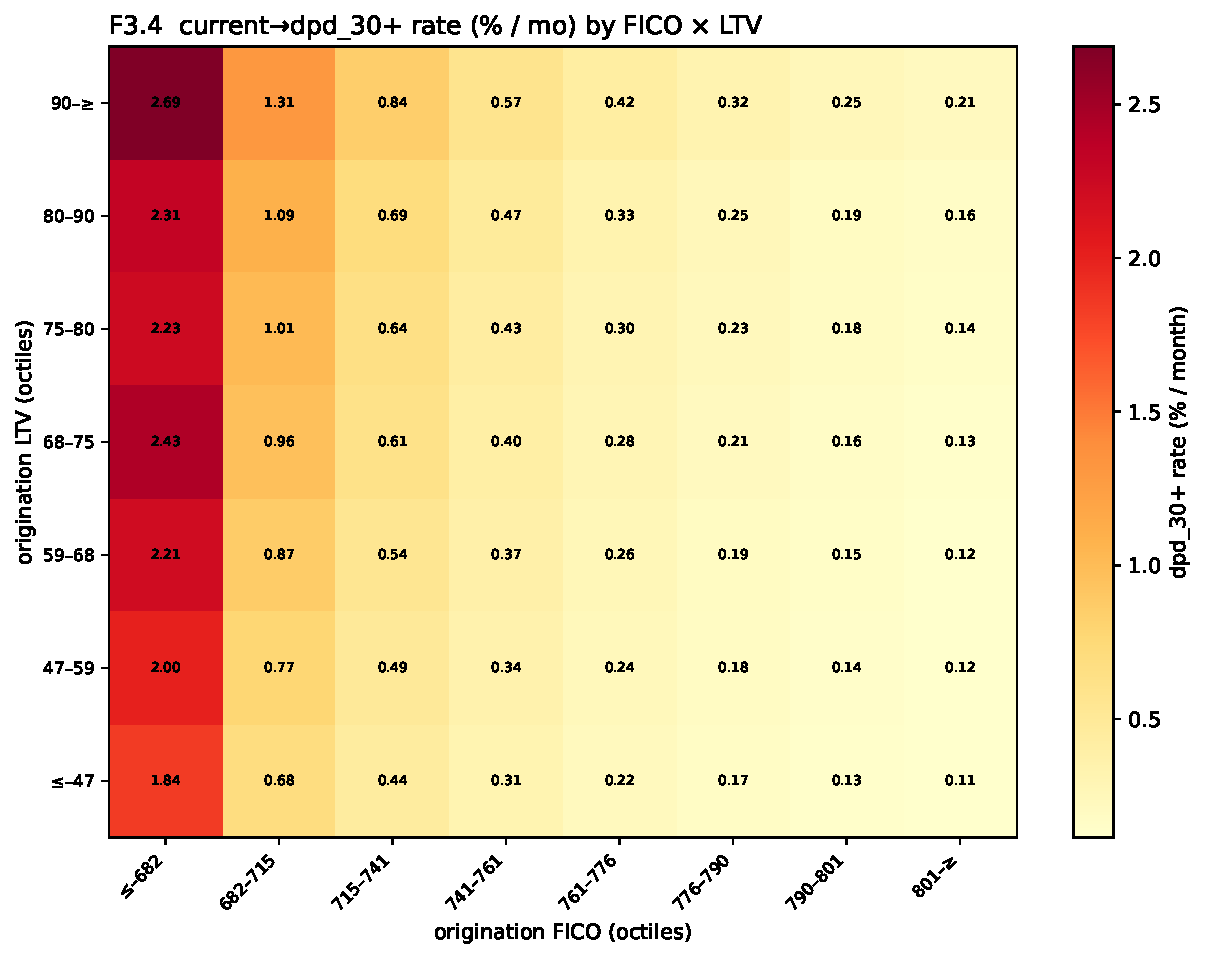
\includegraphics[width=0.78\textwidth]{figs/F3.4_fico_ltv_heatmap.pdf}
\caption[Monthly delinquency-entry rate on a credit-score $\times$ LTV
grid]{Monthly delinquency-entry rate on a credit-score $\times$ LTV grid
(equal-population bands): the additive credit-score gradient grows with
leverage --- additivity is misspecified.}\label{fig:interaction-ficoltv}
\end{figure}

\begin{figure}[htbp]\centering
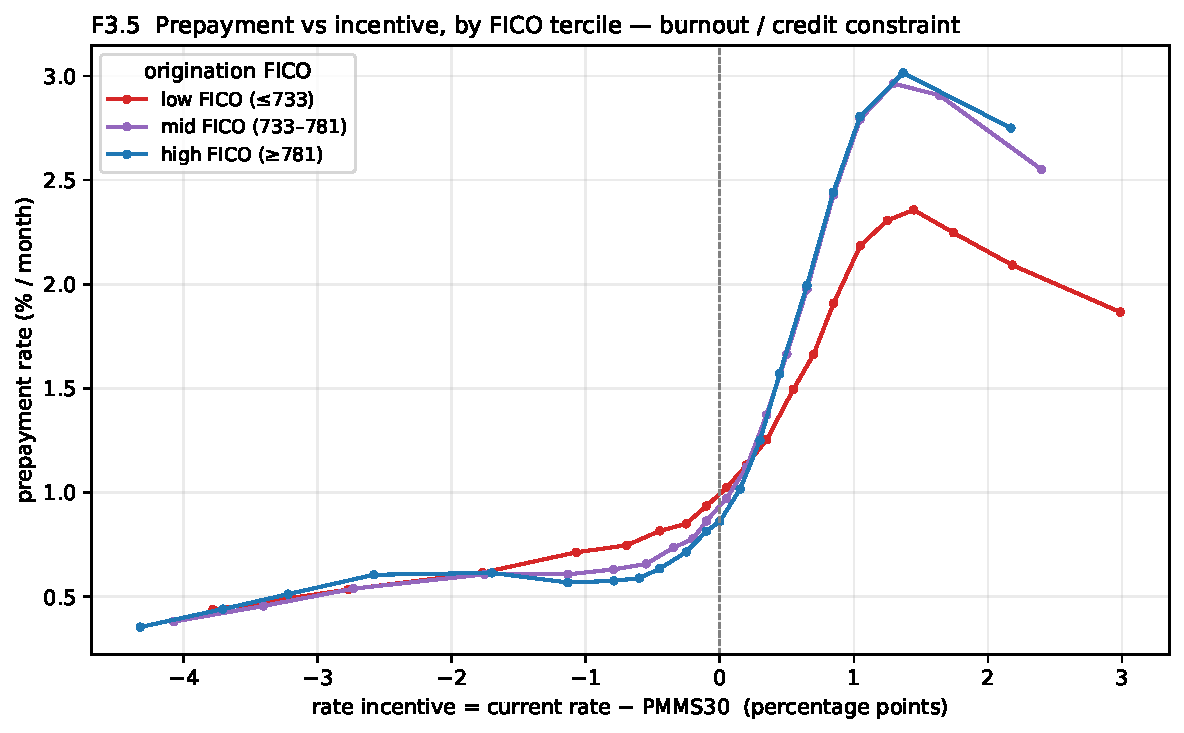
\includegraphics[width=0.8\textwidth]{figs/F3.5_incentive_fico.pdf}
\caption[The incentive S-curve by credit-score tercile]{The incentive
S-curve by credit-score tercile: the refinancing response to an
in-the-money option rises with credit
quality.}\label{fig:interaction-incfico}
\end{figure}

\begin{figure}[htbp]\centering
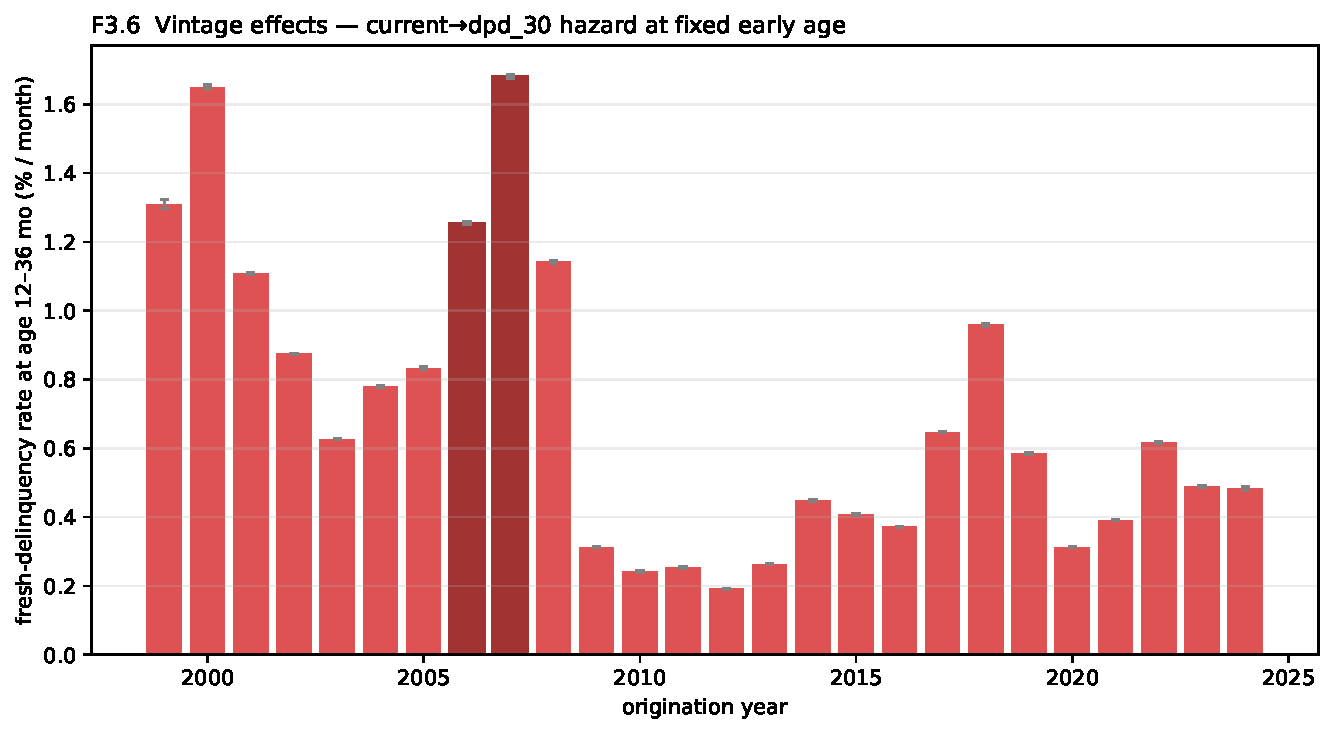
\includegraphics[width=0.8\textwidth]{figs/F3.6_vintage.pdf}
\caption[Delinquency hazard by origination cohort at fixed loan
age]{Delinquency hazard by origination cohort at fixed loan age
(12--36 months): the 2006--08 bubble vintages.}\label{fig:vintage}
\end{figure}

Taken together, the evidence points one way: monthly transition risk
depends on the covariates nonlinearly (the seasoning hump, the
incentive S-curve, convex credit-score decay) and interactively
(score$\times$leverage, incentive$\times$score, vintage).  A
linear-additive model should therefore underfit --- most severely on
prepayment, the channel combining the sharpest single-variable
nonlinearity with a first-order interaction --- and
Chapter~\ref{chap:results} tests precisely this.

% ────────────────────────────────────────────────────────────
\section{Comparison to Sirignano et al.\ (2021)}
\label{sec:data-comparison}

The dataset employed in the present study differs in several important
respects from the proprietary CoreLogic dataset used by
\citet{sirignano2021}, and these differences bear on the
interpretation of the results.

\citet{sirignano2021} draw on records for approximately 120 million
mortgages --- both prime and subprime --- originated across the United
States between January 1995 and June 2014, yielding approximately 3.5
billion loan-month observations.  The CoreLogic data encompass the
full spectrum of mortgage products, including fixed-rate,
adjustable-rate, hybrid, balloon, and interest-only loans, as well as
government-insured instruments.  Macro-economic covariates ---
zip-code-level house price indices from Zillow, county-level
unemployment rates from the Bureau of Labor Statistics, and the
Freddie Mac PMMS series --- are merged at the loan-month level within
the CoreLogic database.  The dataset is proprietary and cannot be
reproduced by independent researchers.

The Fannie Mae primary dataset, by contrast, is limited to
conventional fixed-rate fully-amortising loans and excludes both
subprime and government-insured products.  Macro-economic covariates
must be sourced and joined externally, as described in
Section~\ref{subsec:data-external}.  These differences have two
principal consequences.  First, the estimation sample is more
homogeneous in product mix; the nonlinear prepayment dynamics
associated with adjustable-rate burnout and subprime option exercise
--- prominent in \citeauthor{sirignano2021} --- are absent.  Second,
the absence of a subprime segment limits the range of credit-risk
outcomes observed; \citet{sirignano2021} report a median FICO score
of 630 for their subprime sub-sample against 730 for the prime
sub-sample, whereas the Fannie Mae population is concentrated at the
higher end of this credit-quality spectrum.

These limitations notwithstanding, the Fannie Mae dataset provides a
fully reproducible basis for the analysis.  The core methodological
contribution of \citet{sirignano2021} --- applying deep learning to a
multinomial competing-risks model of monthly loan-state transitions
--- transfers completely to the Fannie Mae panel.  The architecture,
estimation procedure, and evaluation framework described in subsequent
chapters are direct adaptations of that approach.  Table~\ref{tab:data-comparison}
summarises the key differences.

\begin{table}[htbp]
  \centering
  \small
  \begin{tabularx}{\textwidth}{@{} l X X @{}}
    \toprule
    \textbf{Dimension}
      & \textbf{Sirignano et al.\ (2021)}
      & \textbf{Present study} \\
    \midrule
    Data source
      & CoreLogic (proprietary)
      & Fannie Mae SFLP (public) \\[3pt]
    Total loans
      & ${\sim}120$ million
      & 57.6 million \\[3pt]
    Loan-month observations
      & ${\sim}3.5$ billion
      & 3.31 billion \\[3pt]
    Origination window
      & 1995--2014
      & 1999--2025 (full vintage set, reporting to 2025-12) \\[3pt]
    Products covered
      & Fixed, ARM, hybrid, balloon, IO
      & Fixed-rate, fully amortising only \\[3pt]
    Credit segments
      & Prime and subprime
      & Conventional (predominantly prime) \\[3pt]
    Macro covariates
      & Embedded (Zillow, BLS, PMMS)
      & External join required (FHFA HPI, PMMS) \\[3pt]
    Geographic detail
      & Full 5-digit zip code
      & 3-digit truncated zip; MSA \\[3pt]
    States modelled
      & Seven
      & Seven (identical mapping) \\[3pt]
    Reproducibility
      & Not publicly reproducible
      & Fully reproducible \\
    \bottomrule
  \end{tabularx}
  \caption[Comparison of the Fannie Mae SFLP dataset and the
  CoreLogic dataset used by Sirignano et al.\ (2021)]%
  {\textit{Comparison of the Fannie Mae SFLP primary dataset and the
  CoreLogic dataset used by \citet{sirignano2021}.}  CoreLogic counts
  are approximate as reported by the authors; Fannie Mae counts are
  measured on the assembled panel (Section~\ref{sec:data-summary}).}
  \label{tab:data-comparison}
\end{table}

%  to main.tex (after chapter2, before conclusions).
%
%  Required packages (add to the preamble of main.tex):
%      \usepackage{booktabs}
%      \usepackage{tabularx}
%      \usepackage{multirow}
%      \usepackage{natbib}   % or your preferred bib style
% ============================================================

\chapter{Data}
\label{chap:data}

% ────────────────────────────────────────────────────────────
\section{Data Source}
\label{sec:data-source}

This study employs the Fannie Mae Single-Family Loan Performance
(SFLP) dataset, a publicly available research dataset maintained by
the Federal National Mortgage Association (Fannie Mae) and updated on
a quarterly basis.  The dataset was originally released in April 2013
and contains origination and monthly performance records for a subset
of single-family conventional mortgage loans acquired by Fannie Mae
since January 2000.  New loan acquisitions and performance data are
added with an approximate four-month lag following the end of each
calendar quarter \citep{fanniemae2024}.

The data are organised as a \emph{loan-month panel}: each observation
corresponds to a single mortgage loan in a single monthly reporting
period, beginning at the month of acquisition and continuing until the
loan terminates through full prepayment, foreclosure, Real Estate
Owned (REO) disposition, or contractual maturity, or until the data
cut-off date.  This longitudinal structure is well-suited to the
competing-risks framing of \citet{sirignano2021}, which the present
study adapts to the Fannie Mae data.

Raw files are distributed as pipe-delimited CSV without a header row,
organised by acquisition quarter and identified by the convention
\texttt{YYYYQn.csv}.  Column identities are positional, fully
specified in the Fannie Mae Single-Family Loan Performance Data File
Layout and Glossary.  Each row contains 113 fields encoding static
origination attributes, dynamic monthly performance measures, and
post-termination expense and proceeds data.  The estimation sample
employed in this study is the \emph{complete} vintage set from a
single quarterly release: 104 acquisition-quarter files covering
cohorts from 2000Q1 onwards, with monthly reporting periods from
January 2000 through December 2025.  The assembled panel comprises
\textbf{3{,}312{,}456{,}883 loan-month observations across
57{,}562{,}668 loans} --- performance histories spanning four
interest-rate cycles, the 2008--11 foreclosure crisis, the COVID-era
forbearance episode, and the 2022--23 rate shock.

\subsection{From raw files to the estimation panel}
\label{subsec:data-pipeline}

Three distinct concepts in this dataset are colloquially called a
``quarter,'' and distinguishing them prevents the most common
assembly errors.  The \emph{acquisition vintage} identifies a file:
each \texttt{YYYYQn.csv} contains the loans Fannie Mae acquired in
that quarter, carrying their entire subsequent monthly history, and a
loan appears in exactly one file --- so concatenating all files
assembles the full sample with no duplication.  The \emph{monthly
reporting period} identifies a row, and this time dimension --- not
redundancy --- is why the dataset is large.  The \emph{release}
identifies the download: Fannie Mae republishes the entire dataset
quarterly with extended histories, so all files must come from one
release lest vintages carry inconsistent right-censoring dates; an
ingestion audit verifies a uniform cut-off across all 104 files.

Because no single file fits in memory ($\sim$800\,GB of raw CSV in
total), a six-stage pipeline converts the files into a compressed,
columnar store queried out of core: an integrity audit, streaming
conversion, type and sentinel cleaning, construction of the
transition panel with the outcome variable of
Section~\ref{sec:data-outcome}, sampling utilities, and a
reconciliation step that verifies row counts against the raw files.
Columnar storage means a query touching six of the 113 fields reads
roughly five per cent of the bytes, which is what makes the
full-panel descriptive statistics and exploratory analysis of
Sections~\ref{sec:data-summary} and~\ref{sec:data-eda}
computationally cheap.

% ────────────────────────────────────────────────────────────
\section{Population and Eligibility}
\label{sec:data-population}

The primary dataset is not a census of all loans in Fannie Mae's
guarantee book; it is a curated research sample subject to documented
eligibility and exclusion criteria \citep{fanniemae2024}.  The
population is restricted to fixed-rate, fully amortising,
full-documentation single-family conventional mortgage loans with
original terms of at least five years and less than 35 years,
originated on or after 1 January 1999 and acquired by Fannie Mae on
or after 1 January 2000.

A number of product types are explicitly excluded.  Adjustable-rate
mortgages, interest-only loans, balloon-amortisation mortgages, and
loans carrying prepayment penalties are absent from the dataset.
Also excluded are loans with original loan-to-value (LTV) ratios
exceeding 97 per cent, Alt-A and other reduced-documentation
products, government-insured loans (FHA and VA), loans subject to
long-term standby commitments or third-party risk-sharing
arrangements other than primary mortgage insurance, and loans
acquired on a negotiated bulk basis.  Loans with non-standard payment
due dates and loans that liquidated in the same month as acquisition
are similarly excluded.  Fannie Mae's Home Affordable Refinance
Program (HARP) loans are likewise absent from the primary dataset;
when a loan in the primary dataset was subsequently refinanced through
HARP, its termination is recorded as a standard prepayment, and its
post-refinance performance is not tracked here.  This is discussed
further in Section~\ref{sec:data-outcome}.

These restrictions yield a sample of conventionally underwritten
fixed-rate mortgages broadly representative of the agency conventional
loan market under post-crisis underwriting standards.  The exclusion
of adjustable-rate and interest-only products limits the range of
prepayment incentive dynamics captured relative to the full-spectrum
dataset used by \citet{sirignano2021}; this is discussed in
Section~\ref{sec:data-comparison}.  Table~\ref{tab:eligibility}
summarises the principal eligibility criteria and exclusions.

\begin{table}[htbp]
  \centering
  \small
  \begin{tabularx}{\textwidth}{@{} l X @{}}
    \toprule
    \textbf{Criterion} & \textbf{Requirement / Exclusion} \\
    \midrule
    Origination date      & On or after 1 January 1999 \\[2pt]
    Acquisition date      & On or after 1 January 2000 \\[2pt]
    Product type          & Fixed-rate, fully amortising only \\[2pt]
    Loan term             & $5 \leq \mathrm{term} < 35$ years at origination \\[2pt]
    Documentation         & Full documentation only \\[2pt]
    LTV at origination    & $\leq 97\%$ \\[4pt]
    \emph{Excluded: product}      & ARM, interest-only, balloon,
                                    prepayment-penalty loans \\[2pt]
    \emph{Excluded: credit class} & Alt-A, reduced-documentation,
                                    streamlined processing \\[2pt]
    \emph{Excluded: guarantee}    & Government-insured (FHA, VA) loans \\[2pt]
    \emph{Excluded: structure}    & Long-term standby commitments;
                                    bulk acquisitions; lender-recourse
                                    loans (except primary MI) \\[2pt]
    \emph{Excluded: programme}    & HARP and Refi Plus loans \\[2pt]
    \emph{Excluded: payment}      & Bi-weekly and non-first-of-month
                                    due dates \\[2pt]
    \emph{Excluded: timing}       & Loans liquidated in month of
                                    acquisition \\
    \bottomrule
  \end{tabularx}
  \caption[Eligibility criteria for the Fannie Mae SFLP primary dataset]%
  {\textit{Eligibility criteria for the Fannie Mae SFLP primary
  dataset.}  Source: Fannie Mae Single-Family Loan Performance
  Dataset FAQs \citep{fanniemae2024}.}
  \label{tab:eligibility}
\end{table}

% ────────────────────────────────────────────────────────────
\section{Variables}
\label{sec:data-variables}

The 113 fields in each monthly observation can be organised into three
functional groups: static origination attributes, dynamic monthly
performance attributes, and post-termination resolution data.  The
model uses a subset of these fields as covariates.  Two fields --- the
Current Loan Delinquency Status and the Zero Balance Code --- serve as
the primary inputs from which the outcome variable is constructed.

% ────────────────────────────────
\subsection{Origination Attributes}
\label{subsec:data-origination}

Static origination attributes are recorded at loan delivery and do
not change over the life of the loan absent a modification.  The
borrower's FICO credit score at origination is available for both the
primary borrower and, where applicable, a co-borrower; prior to the
January 2015 dataset release only the lower of the two scores was
disclosed, and a missingness indicator is constructed accordingly.
Continuous origination covariates include the original
debt-to-income (DTI) ratio, original LTV ratio, original combined LTV
(CLTV, which incorporates subordinate liens), original unpaid
principal balance (UPB), original interest rate, and original loan
term in months.  Categorical origination attributes include the
acquisition channel (retail, broker, or correspondent), loan purpose
(purchase, rate-term refinance, or cash-out refinance), property type,
occupancy status (primary residence, second home, or investment
property), property state, Metropolitan Statistical Area (MSA), and
three-digit truncated zip code.  The truncation of the zip code
reflects borrower privacy considerations; full zip codes are not
disclosed in the dataset \citep{fanniemae2024}.

% ────────────────────────────────
\subsection{Dynamic Performance Attributes}
\label{subsec:data-performance}

Dynamic performance attributes are updated in each monthly reporting
period.  The current actual unpaid principal balance reflects the
outstanding loan balance at each point in time.  Loan age, measured
in months from the first payment date, and the remaining months to
legal maturity are derived from the contractual amortisation schedule.
The current interest rate reflects the applicable note rate, updated
when a modification changes the loan terms.

Two dynamic fields jointly determine the outcome variable.  The
\textbf{Current Loan Delinquency Status} reports the number of missed
monthly payments as a two-character code: \texttt{00} denotes a
current loan; \texttt{01}, \texttt{02}, and codes \texttt{03} and
above denote 30-, 60-, and 90-or-more-day delinquencies respectively;
and \texttt{XX} denotes an unavailable status.  The \textbf{Zero
Balance Code} is populated exclusively in the terminal monthly
observation and classifies the manner of loan termination into nine
categories, distinguishing between voluntary prepayments, third-party
foreclosure sales, short sales, repurchases, REO dispositions, note
sales, and non-credit removals.  (The dataset also carries a 24-month
payment-history string; it is not used as a model input here, since
the current state and loan-level covariates already summarise the
information the transition model conditions on.)

% ────────────────────────────────
\subsection{Externally Sourced Covariates}
\label{subsec:data-external}

A small, fixed set of external macroeconomic series is joined to the
loan-level panel at feature-construction time (the stored panel
itself is never rewritten); Table~\ref{tab:macrovars} summarises the
sources.  The Freddie Mac Primary Mortgage Market Survey (PMMS)
weekly fixed-rate series, aggregated to calendar-month means, supplies
the prevailing market mortgage rate from which the \emph{rate
incentive} of Equation~\eqref{eq:incentive} is computed --- the
refinancing option value, the primary driver of prepayment behaviour
in the empirical mortgage literature
\citep{schwartz1989,sirignano2021}.  Unemployment rates enter at both
national (Bureau of Labor Statistics) and state level, the latter
because the cross-sectional dispersion in labour-market conditions
(Nevada versus Texas in 2009) is precisely the variation a national
series cannot supply.  House prices enter through the Freddie Mac
House Price Index at national and state level, from which the
mark-to-market loan-to-value ratio of Equation~\eqref{eq:mtmltv} ---
the principal determinant of the default option value
\citep{deng2000} --- and the trailing twelve-month house-price change
are constructed.  The ten-year Treasury yield completes the set.

Each series is joined with a \emph{publication lag} reflecting when
the value was actually observable: rates are published in real time
(no lag), month-$t$ unemployment is released early in month $t{+}1$
(one-month lag), and the house-price index roughly two months after
the reference month (two-month lag).  Final-revision series are used
rather than real-time vintages --- a stated limitation, standard for
historical studies.  Where a state-level value is unavailable
(territories; series start dates) the national value substitutes,
with an indicator flag carried as a model feature.

\begin{table}[htbp]
  \centering
  \small
  \begin{tabularx}{\textwidth}{@{} l l l l c @{}}
    \toprule
    \textbf{Variable} & \textbf{Source} & \textbf{Geography}
      & \textbf{Monthly value} & \textbf{Lag} \\
    \midrule
    30-yr mortgage rate & Freddie Mac PMMS & national & month mean & 0\,m \\
    10-yr Treasury yield & FRED \texttt{DGS10} & national & month mean & 0\,m \\
    Unemployment rate & BLS (via FRED) & national + state & as published & 1\,m \\
    House-price index & Freddie Mac FMHPI & national + state & as published & 2\,m \\
    \bottomrule
  \end{tabularx}
  \caption[External macroeconomic covariates and join conventions]%
  {\textit{External macroeconomic covariates and join conventions.}
  A loan-month at calendar month $t$ is joined to the macro value of
  month $t-\ell$, where $\ell$ is the publication lag.  Seasonally
  adjusted versions are used throughout.}
  \label{tab:macrovars}
\end{table}

As a check on the incentive variable, a market-rate proxy derived
from the panel itself --- the average note rate of loans originated
in each calendar month --- tracks the PMMS series with correlation
$0.991$, root-mean-square deviation $0.198$ percentage points, and
mean absolute deviation $0.147$ percentage points, with a mean gap of
essentially zero.  The PMMS-based incentive is the primary feature;
the panel-derived proxy is retained as a robustness alternative,
demonstrating that the incentive variable is not an artefact of one
data source.

% ────────────────────────────────────────────────────────────
\section{Outcome Variable}
\label{sec:data-outcome}

Following \citet{sirignano2021}, the outcome variable is a categorical
measure of mortgage state in month $t+1$, conditional on the loan's
state and covariate vector in month $t$.  Seven mutually exclusive
states are defined: \emph{Current}, \emph{30 Days Past Due}
(30\,DPD), \emph{60 Days Past Due} (60\,DPD), \emph{90+ Days Past
Due} (90+\,DPD), \emph{Foreclosure}, \emph{Real Estate Owned} (REO),
and \emph{Prepaid}.

State assignment for each loan-month observation follows a
deterministic hierarchy.  When the Zero Balance Code is present ---
indicating the terminal observation for the loan --- the termination
type is mapped to the Foreclosure, REO, or Prepaid absorbing state as
shown in Table~\ref{tab:state-mapping}.  When the Zero Balance Code is
absent, the delinquency status field governs: codes \texttt{00}
through \texttt{03} and above map to Current, 30\,DPD, 60\,DPD, and
90+\,DPD respectively, while \texttt{XX} is treated as missing.  The
state in month $t+1$ is obtained by a window lead over the reporting
period dimension, partitioned by loan identifier.  Loans whose final
observation falls at or before the data cut-off without a recorded
termination event receive a censored indicator and are excluded from
the labelled target.

Regarding HARP loans: as noted in Section~\ref{sec:data-population},
any loan in the primary dataset that was refinanced through the
HARP programme terminates with a Zero Balance Code of \texttt{01}
(prepaid) at the moment of refinancing and is therefore treated as a
standard prepayment in the outcome variable.  This approximation is
defensible given that the loan is extinguished from Fannie Mae's
credit exposure in either case, though it may marginally overstate
the rate-incentive sensitivity of the prepayment hazard during the
period of peak HARP activity (approximately 2009--2013).

\begin{table}[htbp]
  \centering
  \small
  \begin{tabularx}{\textwidth}{@{} l l l X @{}}
    \toprule
    \textbf{State} & \textbf{Source field} & \textbf{Condition}
      & \textbf{Economic interpretation} \\
    \midrule
    Current
      & Delinquency Status & \texttt{= 00}
      & Borrower is contractually current on all payments. \\[3pt]
    30\,DPD
      & Delinquency Status & \texttt{= 01}
      & One missed monthly payment. \\[3pt]
    60\,DPD
      & Delinquency Status & \texttt{= 02}
      & Two consecutive missed monthly payments. \\[3pt]
    90+\,DPD
      & Delinquency Status & \texttt{$\geq$ 03}
      & Three or more missed payments; serious delinquency. \\[3pt]
    Foreclosure
      & Zero Balance Code  & \texttt{02, 03, 15,}
      & Credit-loss termination: third-party sale, short sale, \\
      &                    & \texttt{97, 98}
      & note sale, or credit-event repurchase. \\[3pt]
    REO
      & Zero Balance Code  & \texttt{= 09}
      & Fannie Mae acquires ownership of the property. \\[3pt]
    Prepaid
      & Zero Balance Code  & \texttt{01, 06, 16,}
      & Full payoff, contractual maturity, repurchase, \\
      &                    & \texttt{96}
      & or non-credit removal (including HARP exits). \\
    \bottomrule
  \end{tabularx}
  \caption[Mapping of Fannie Mae data fields to the seven-state
  outcome variable]%
  {\textit{Mapping of Fannie Mae data fields to the seven-state
  outcome variable.}  The Zero Balance Code is populated only in the
  terminal monthly observation; the Delinquency Status governs state
  assignment in all non-terminal periods.}
  \label{tab:state-mapping}
\end{table}

One structural feature of this dataset deserves emphasis: because the
Foreclosure, REO, and Prepaid states are derived from the Zero
Balance Code --- populated only in a loan's final observation ---
these three states are \emph{absorbing}.  There is no ongoing ``in
foreclosure'' monthly status as in the CoreLogic data of
\citet{sirignano2021}, where loans in formal foreclosure are observed
month by month and occasionally return to performing status.  The
origin set here therefore comprises the four live states (Current
through 90+\,DPD) while destinations span all seven: the transition
matrix is $4\times 7$ rather than $7\times 7$
(Section~\ref{sec:meth-model}).  Within the live states the data are
rich in both directions --- delinquency deepens at most one bucket
per month, but cures can jump multiple buckets, and a meaningful
fraction of seriously delinquent loans return to current.  The
seven-state formulation captures this in a way that a binary
default-versus-prepayment classification would obscure, and the
empirical monthly transition matrix derived from each training window
serves as the floor benchmark for the model comparison
(Section~\ref{subsec:meth-empirical}).

% ────────────────────────────────────────────────────────────
\section{Panel Composition and Summary Statistics}
\label{sec:data-summary}

The assembled panel comprises 3{,}312{,}456{,}883 loan-month
observations across 57{,}562{,}668 loans in 104 acquisition-vintage
partitions, with reporting months from January 2000 through December
2025.  Table~\ref{tab:stateshares} reports the distribution of
loan-months across the seven states.  Two features dominate.  First,
extreme class imbalance: the Current state accounts for $96.28\%$ of
all loan-months, while the credit-event terminals occur at roughly
one in ten thousand observations --- the empirical fact behind both
the importance-weighted thinning of training data
(Section~\ref{sec:meth-design}) and the Laplace smoothing of the
empirical benchmark (Section~\ref{subsec:meth-empirical}).  Second,
the rare states are nonetheless abundantly populated in absolute
terms (REO alone contributes roughly half a million loan-months),
which is what permits stable estimation of rare-transition
probabilities at this scale.

\begin{table}[htbp]
  \centering
  \small
  \begin{tabular}{l r @{\qquad\qquad} l r}
    \toprule
    \textbf{State} & \textbf{Share} & \textbf{State} & \textbf{Share} \\
    \midrule
    Current  & 96.28\,\% & 60\,DPD     & 0.31\,\%   \\
    Prepaid  & 1.25\,\%  & REO         & 0.014\,\%  \\
    30\,DPD  & 1.15\,\%  & Foreclosure & 0.0067\,\% \\
    90+\,DPD & 0.98\,\%  &             &            \\
    \bottomrule
  \end{tabular}
  \caption[Distribution of loan-months across the seven states]%
  {\textit{Distribution of loan-months across the seven states},
  full panel, 2000--2025 (3.31 billion loan-months).}
  \label{tab:stateshares}
\end{table}

Pooled over time, the monthly transition rates out of Current are
$1.27\%$ to Prepaid and $0.64\%$ to 30\,DPD.  The pooling, however,
hides the economics: Figure~\ref{fig:transitionrates} plots the
monthly series over 2000--2025, displaying the 2003 and 2020--21
refinancing waves in the prepayment rate, the 2008--11 default wave
in the delinquency rates, and the sharp 2022--23 collapse in
prepayments as market rates rose.  These regime shifts --- rather
than any single structural break --- are the empirical justification
for the rolling backtest design of Section~\ref{sec:meth-design}.
During 2020--21 the delinquency-status codes additionally reflect
COVID-era forbearance, which manifests as unusual persistence in
delinquency states followed by elevated cure rates; no special
treatment is applied, but results involving those years are read with
this in mind.

\begin{figure}[htbp]\centering
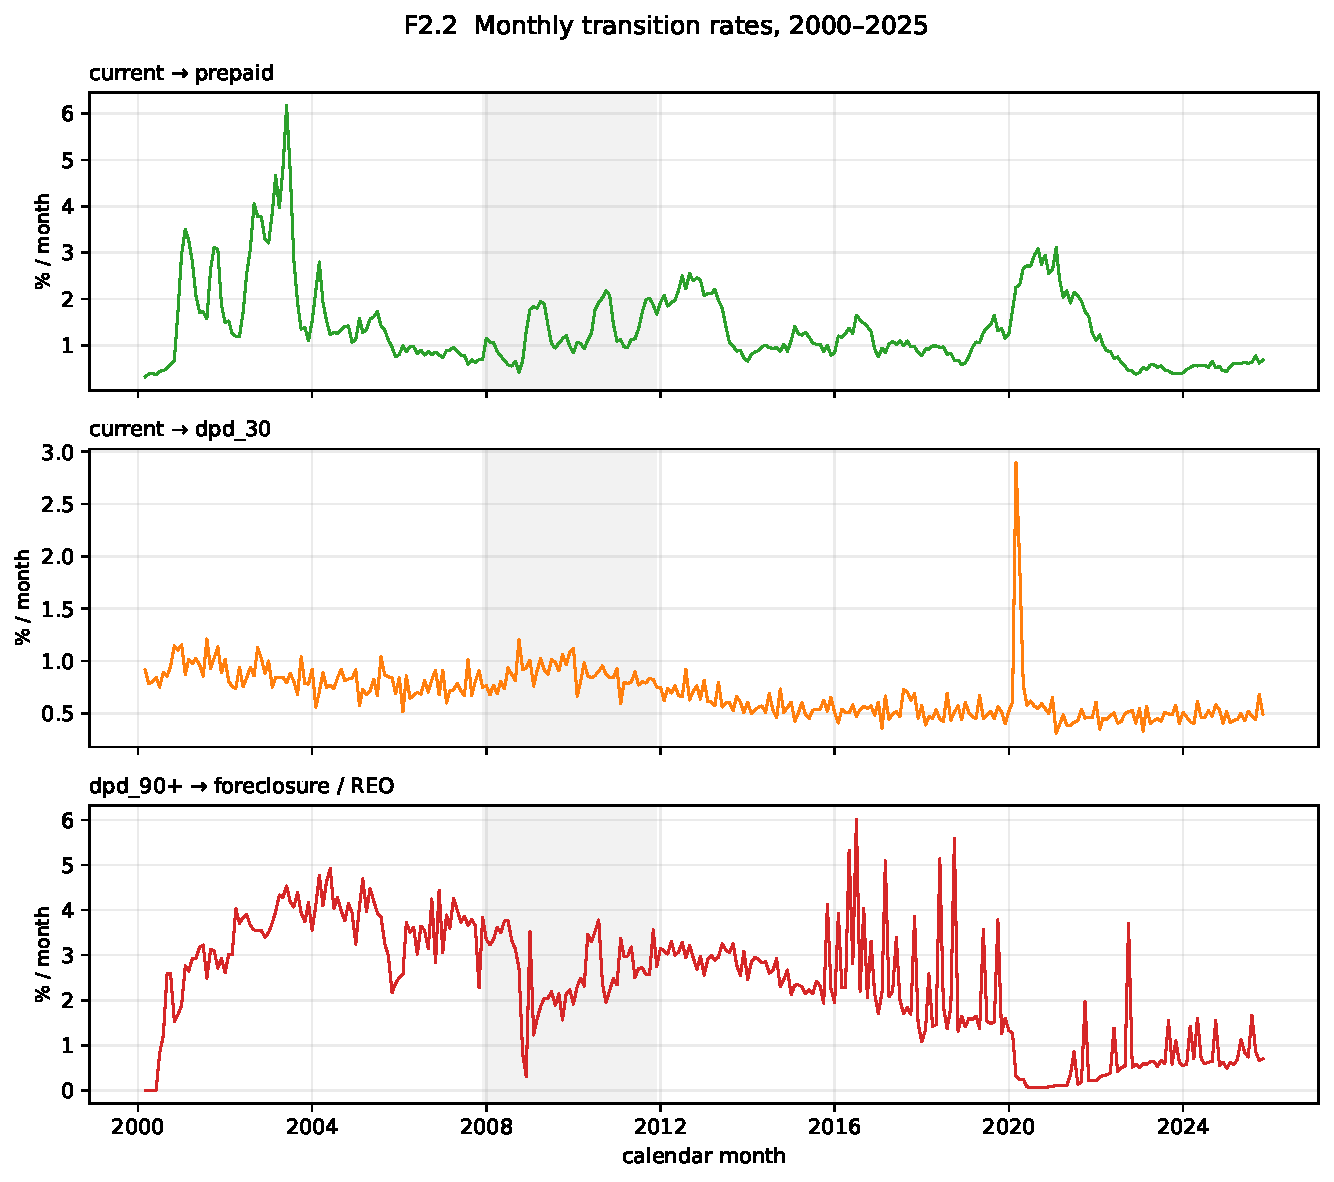
\includegraphics[width=0.9\textwidth]{figs/F2.2_transition_rates.pdf}
\caption[Monthly transition rates out of the Current state]{Monthly
transition rates out of the Current state, 2000--2025: prepayment and
entry into 30\,DPD (left axis), serious-delinquency terminations
(right axis).  Vertical shading marks the 2008--11 crisis and the
2020--21 forbearance episode.}\label{fig:transitionrates}
\end{figure}

\begin{table}[htbp]\centering\small
\caption[Summary statistics of model covariates]{Summary statistics of
the continuous model covariates over the full panel: null rate, mean,
standard deviation, and the min/1st/25th/50th/75th/99th/max
percentiles.}\label{tab:covariate-summary}
\resizebox{\textwidth}{!}{% Source: outputs/tables/eda/T1.2_covariate_summary_continuous.tex (full-panel
% Stage-6 QA). Tabular-only; wrap in \resizebox in chapter3.tex. Caption+label there.
\begin{tabular}{lrrrrrrrrrrl}
\toprule
column & null\_rate & mean & std & min & p01 & p25 & median & p75 & p99 & max & log\_flagged \\
\midrule
Original Interest Rate & 0 & 4.71882 & 1.32648 & 1.5 & 2.36602 & 3.62711 & 4.62688 & 5.75 & 7.85794 & 16.5 & False \\
Current Interest Rate & 0.012707 & 4.68763 & 1.32523 & 0 & 2.28982 & 3.625 & 4.60188 & 5.75 & 7.83746 & 13.5 & False \\
Original UPB & 0 & 199755 & 121639 & 1000 & 38809.4 & 109817 & 170562 & 262260 & 596156 & 2.326e+06 & True \\
Current Actual UPB & 0 & 159715 & 124113 & 0 & 0 & 71875.9 & 134287 & 224204 & 564970 & 2.86e+06 & True \\
Original Loan Term & 0 & 306.643 & 82.0617 & 36 & 120 & 202.959 & 360 & 360 & 360 & 360 & False \\
Loan Age & 0.01272 & 46.8107 & 42.4782 & -3 & 0 & 15 & 34.9747 & 65.8525 & 188.817 & 322 & False \\
Remaining Months to Maturity & 0.027474 & 252.795 & 97.4912 & 0 & 22.5446 & 167.472 & 294.279 & 335.84 & 359 & 480 & False \\
Original Loan-to-Value (LTV) & 0 & 69.7447 & 17.8489 & 1 & 21.1656 & 59.0522 & 74.5451 & 80 & 97 & 105 & False \\
Original Combined LTV (CLTV) & 0.003362 & 70.4277 & 17.9251 & 1 & 21.6837 & 59.7414 & 75 & 80 & 97 & 199 & False \\
Debt-to-Income (DTI) & 0.014108 & 33.3364 & 11.2275 & 0 & 9.02377 & 25 & 33.6755 & 41.9385 & 60.056 & 64 & False \\
fico\_orig & 0.002844 & 746.693 & 52.418 & 300 & 603.635 & 712.774 & 759.539 & 788.96 & 817.552 & 850 & False \\
fico\_co & 0.515382 & 754.702 & 49.6835 & 300 & 611.863 & 725.849 & 768.606 & 793.443 & 818.68 & 850 & False \\
Mortgage Insurance Percentage & 0.810875 & 24.1429 & 7.26184 & 0.12 & 6 & 22.29 & 25 & 30 & 35 & 50 & False \\
Number of Borrowers & 0.000119 & 1.55013 & 0.514524 & 1 & 1 & 1 & 2 & 2 & 2 & 10 & False \\
Number of Units & 0 & 1.03643 & 0.248099 & 1 & 1 & 1 & 1 & 1 & 2 & 4 & False \\
\bottomrule
\end{tabular}
}
\end{table}

% ────────────────────────────────────────────────────────────
\section{Exploratory Evidence: Nonlinearity and Interactions}
\label{sec:data-eda}

Before any model is fitted, the case that nonlinear modelling is
\emph{needed} can be made by counting alone.  The instrument is the
empirical hazard curve: bucket a covariate into equal-population
bins and plot the realised one-month transition rate per bin, with
Wilson 95\% confidence intervals.  Because each curve is a single
out-of-core aggregation over the columnar panel, the entire
programme runs in minutes.

\subsection{Single-covariate nonlinearity}
\label{subsec:data-eda-single}

Three hazard curves carry the argument.
\emph{Prepayment versus loan age}
(Figure~\ref{fig:hazard-age}): the rate rises from $0.27\%$ per month
at origination to a peak of $1.56\%$ at approximately 17 months of
age, then decays to $1.11\%$ by month 52 --- the classic
``seasoning hump,'' strongly non-monotone, with a secondary late-life
rise among long-surviving loans.  \emph{Prepayment versus the
refinancing incentive} (Figure~\ref{fig:hazard-incentive}): the rate
is flat at $0.4$--$0.6\%$ per month while the option is out of the
money, turns up sharply through zero, peaks at $2.71\%$ near
$+1.5$ percentage points of incentive, and falls back to $2.16\%$ by
$+2.7$ --- a roughly sevenfold range containing both an inflection
and a turning point, reproducing the flagship nonlinearity of
\citet{sirignano2021} on this cleaner credit box.
\emph{Delinquency versus credit score}
(Figure~\ref{fig:hazard-fico}): the entry rate into 30\,DPD falls
twenty-four-fold, from $3.06\%$ per month at FICO ${\approx}623$ to
$0.13\%$ at FICO ${\approx}815$, and the decay is convex --- the
slope in the low-score half is roughly $3.7$ times that in the
high-score half.  None of the three shapes is representable by a
linear term.

\begin{figure}[htbp]\centering
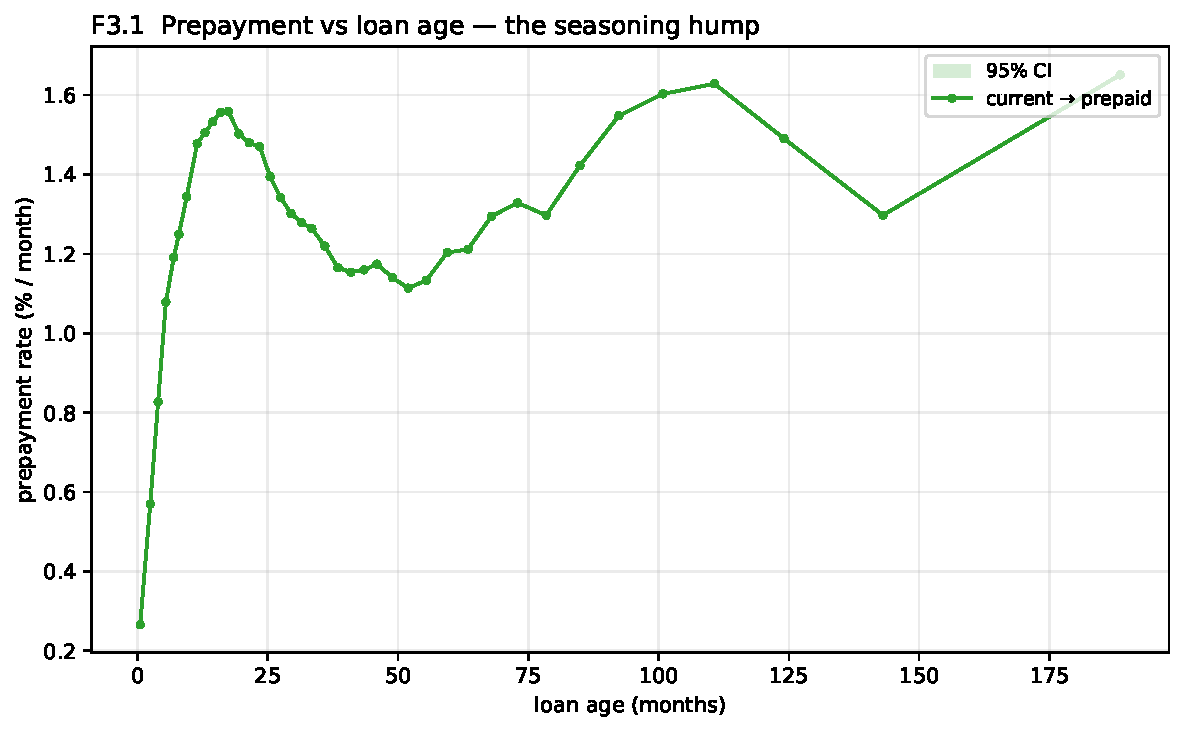
\includegraphics[width=0.8\textwidth]{figs/F3.1_prepay_age.pdf}
\caption[Empirical prepayment hazard by loan age]{Empirical prepayment
hazard by loan age (equal-population buckets, Wilson 95\% intervals):
the seasoning hump.}\label{fig:hazard-age}
\end{figure}

\begin{figure}[htbp]\centering
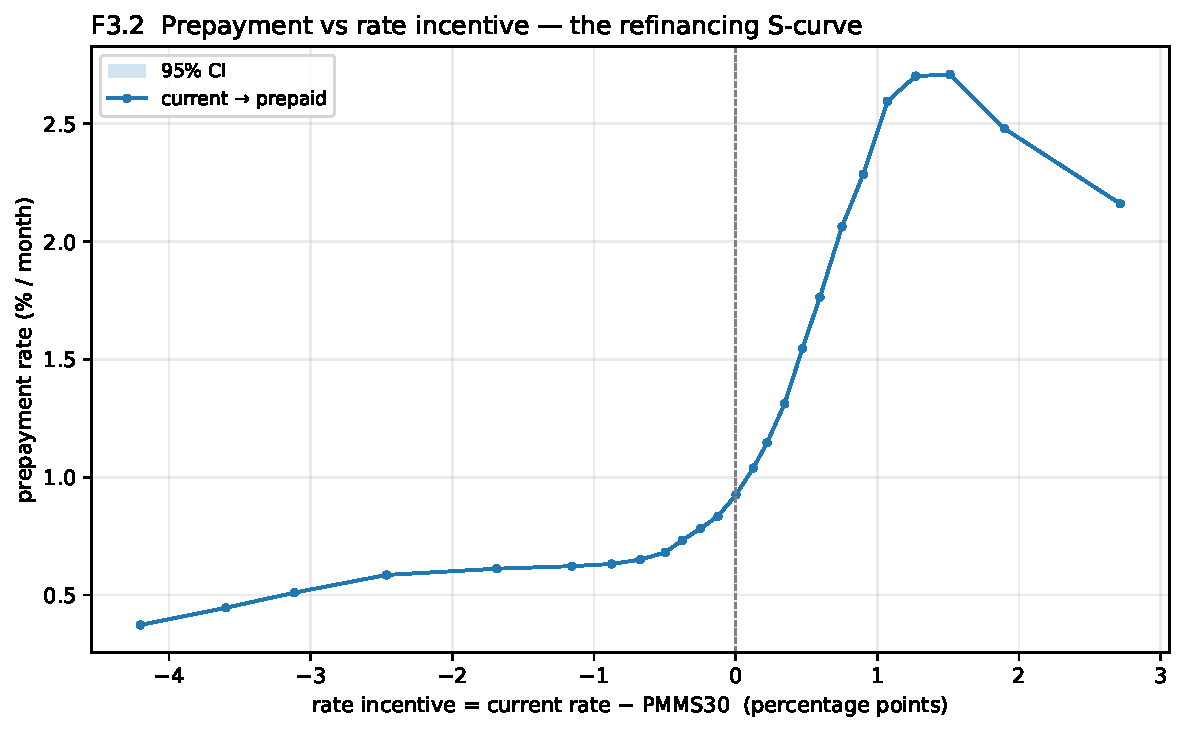
\includegraphics[width=0.8\textwidth]{figs/F3.2_prepay_incentive.pdf}
\caption[Empirical prepayment hazard by refinancing incentive]{Empirical
prepayment hazard by refinancing incentive: the S-curve, with burnout
beyond $+1.5$\,pp.}\label{fig:hazard-incentive}
\end{figure}

\begin{figure}[htbp]\centering
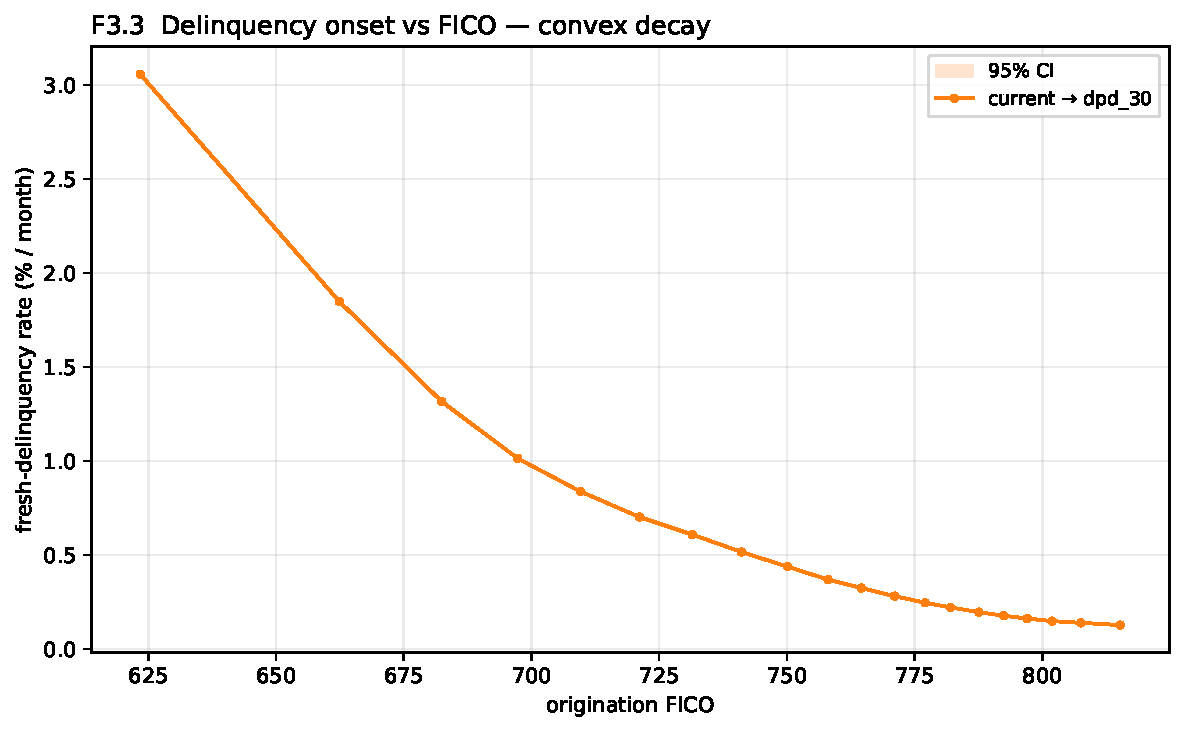
\includegraphics[width=0.8\textwidth]{figs/F3.3_delinq_fico.pdf}
\caption[Empirical 30\,DPD entry hazard by origination credit
score]{Empirical 30\,DPD entry hazard by origination credit score:
convex decay.}\label{fig:hazard-fico}
\end{figure}

\subsection{Interactions: the case against additivity}
\label{subsec:data-eda-interactions}

A linear-\emph{additive} model could in principle be patched with
transformed single-variable terms; interactions are what it cannot
absorb.  On a credit-score~$\times$~LTV grid
(Figure~\ref{fig:interaction-ficoltv}), the monthly rate of entry
into delinquency ranges from $0.11\%$ (best scores, lowest leverage)
to $2.69\%$ (worst scores, highest leverage) --- and decisively, the
\emph{additive} credit-score gradient (worst-minus-best rate) grows
from $1.73$ percentage points at low LTV to $2.48$ at high LTV, a
$43\%$ increase; equivalently, the leverage effect is roughly
$8.5$ times larger for low-score than high-score borrowers.
Additivity forces this gradient to be constant; the violation sits
exactly in the low-score/high-leverage corner that drives credit
losses.  In the prepayment channel
(Figure~\ref{fig:interaction-incfico}), splitting the incentive
S-curve by credit-score tercile shows the in-the-money refinancing
response \emph{rising} with credit quality --- $2.36\%$ per month in
the lowest tercile against $3.01\%$ in the highest --- because
credit-constrained borrowers cannot exercise the option: the
incentive \emph{slope} itself depends on the score.  Finally, holding
loan age fixed at 12--36 months to strip out seasoning, the
delinquency hazard by origination cohort isolates a clean vintage
effect: the 2007 cohort peaks at $1.68\%$ per month against $0.47\%$
for calm cohorts --- a $3.6$-fold premium
(Figure~\ref{fig:vintage}) --- so the origination vintage is a
feature in its own right, not reducible to contemporaneous
covariates.

\begin{figure}[htbp]\centering
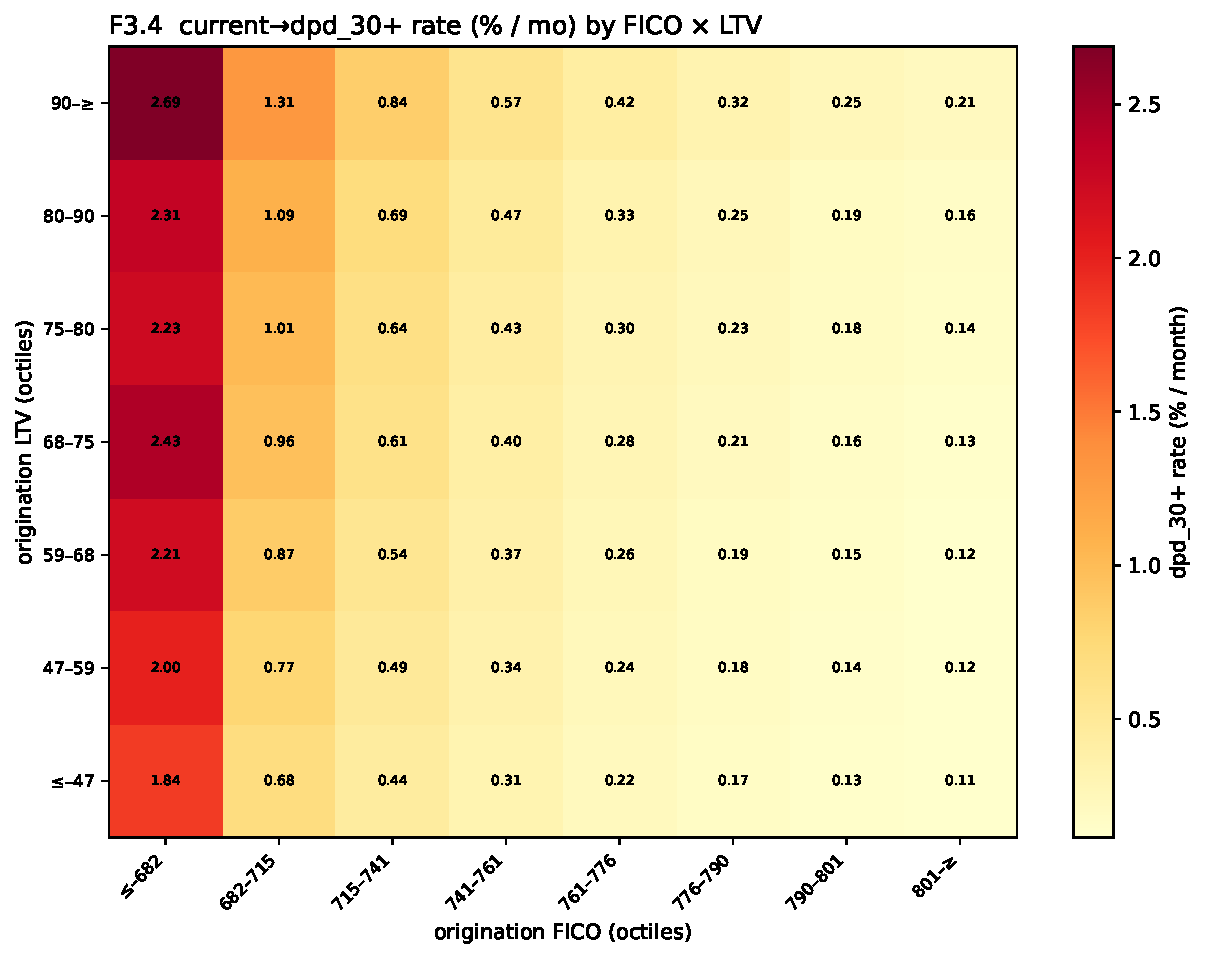
\includegraphics[width=0.78\textwidth]{figs/F3.4_fico_ltv_heatmap.pdf}
\caption[Monthly delinquency-entry rate on a credit-score $\times$ LTV
grid]{Monthly delinquency-entry rate on a credit-score $\times$ LTV grid
(equal-population bands): the additive credit-score gradient grows with
leverage --- additivity is misspecified.}\label{fig:interaction-ficoltv}
\end{figure}

\begin{figure}[htbp]\centering
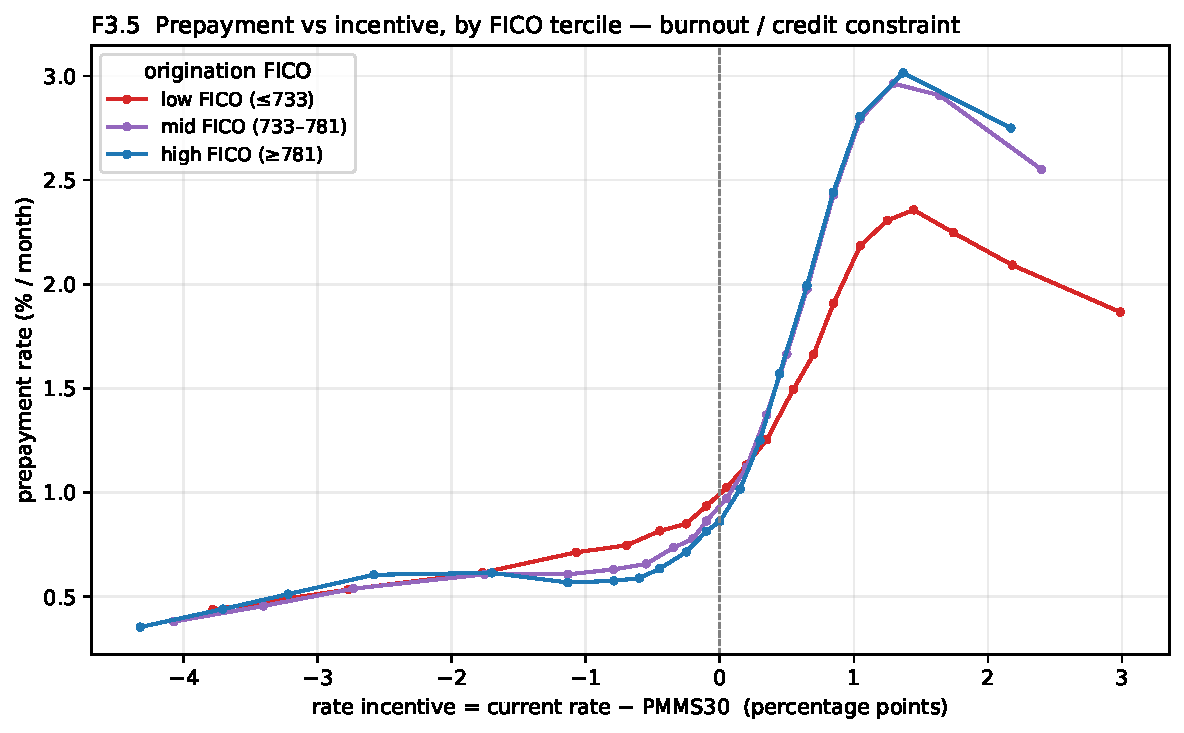
\includegraphics[width=0.8\textwidth]{figs/F3.5_incentive_fico.pdf}
\caption[The incentive S-curve by credit-score tercile]{The incentive
S-curve by credit-score tercile: the refinancing response to an
in-the-money option rises with credit
quality.}\label{fig:interaction-incfico}
\end{figure}

\begin{figure}[htbp]\centering
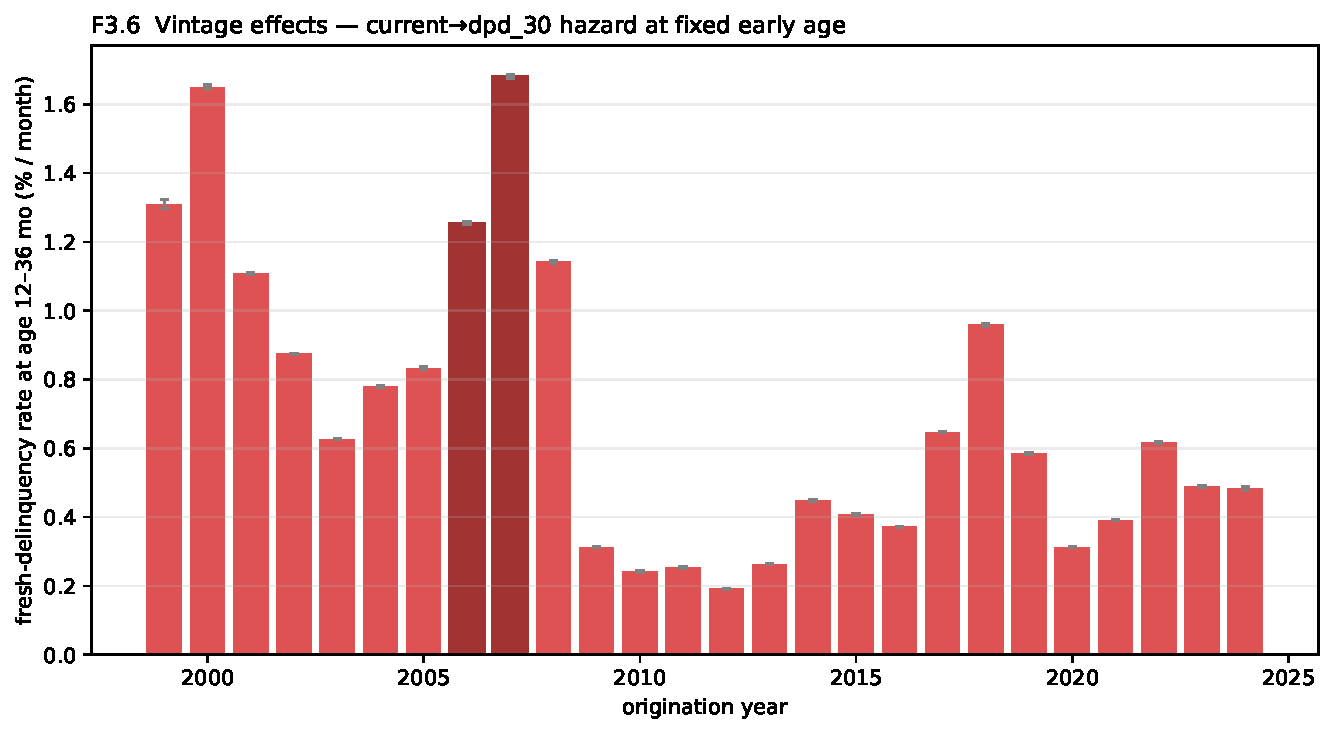
\includegraphics[width=0.8\textwidth]{figs/F3.6_vintage.pdf}
\caption[Delinquency hazard by origination cohort at fixed loan
age]{Delinquency hazard by origination cohort at fixed loan age
(12--36 months): the 2006--08 bubble vintages.}\label{fig:vintage}
\end{figure}

Taken together, the evidence points one way: monthly transition risk
depends on the covariates nonlinearly (the seasoning hump, the
incentive S-curve, convex credit-score decay) and interactively
(score$\times$leverage, incentive$\times$score, vintage).  A
linear-additive model should therefore underfit --- most severely on
prepayment, the channel combining the sharpest single-variable
nonlinearity with a first-order interaction --- and
Chapter~\ref{chap:results} tests precisely this.

% ────────────────────────────────────────────────────────────
\section{Comparison to Sirignano et al.\ (2021)}
\label{sec:data-comparison}

The dataset employed in the present study differs in several important
respects from the proprietary CoreLogic dataset used by
\citet{sirignano2021}, and these differences bear on the
interpretation of the results.

\citet{sirignano2021} draw on records for approximately 120 million
mortgages --- both prime and subprime --- originated across the United
States between January 1995 and June 2014, yielding approximately 3.5
billion loan-month observations.  The CoreLogic data encompass the
full spectrum of mortgage products, including fixed-rate,
adjustable-rate, hybrid, balloon, and interest-only loans, as well as
government-insured instruments.  Macro-economic covariates ---
zip-code-level house price indices from Zillow, county-level
unemployment rates from the Bureau of Labor Statistics, and the
Freddie Mac PMMS series --- are merged at the loan-month level within
the CoreLogic database.  The dataset is proprietary and cannot be
reproduced by independent researchers.

The Fannie Mae primary dataset, by contrast, is limited to
conventional fixed-rate fully-amortising loans and excludes both
subprime and government-insured products.  Macro-economic covariates
must be sourced and joined externally, as described in
Section~\ref{subsec:data-external}.  These differences have two
principal consequences.  First, the estimation sample is more
homogeneous in product mix; the nonlinear prepayment dynamics
associated with adjustable-rate burnout and subprime option exercise
--- prominent in \citeauthor{sirignano2021} --- are absent.  Second,
the absence of a subprime segment limits the range of credit-risk
outcomes observed; \citet{sirignano2021} report a median FICO score
of 630 for their subprime sub-sample against 730 for the prime
sub-sample, whereas the Fannie Mae population is concentrated at the
higher end of this credit-quality spectrum.

These limitations notwithstanding, the Fannie Mae dataset provides a
fully reproducible basis for the analysis.  The core methodological
contribution of \citet{sirignano2021} --- applying deep learning to a
multinomial competing-risks model of monthly loan-state transitions
--- transfers completely to the Fannie Mae panel.  The architecture,
estimation procedure, and evaluation framework described in subsequent
chapters are direct adaptations of that approach.  Table~\ref{tab:data-comparison}
summarises the key differences.

\begin{table}[htbp]
  \centering
  \small
  \begin{tabularx}{\textwidth}{@{} l X X @{}}
    \toprule
    \textbf{Dimension}
      & \textbf{Sirignano et al.\ (2021)}
      & \textbf{Present study} \\
    \midrule
    Data source
      & CoreLogic (proprietary)
      & Fannie Mae SFLP (public) \\[3pt]
    Total loans
      & ${\sim}120$ million
      & 57.6 million \\[3pt]
    Loan-month observations
      & ${\sim}3.5$ billion
      & 3.31 billion \\[3pt]
    Origination window
      & 1995--2014
      & 1999--2025 (full vintage set, reporting to 2025-12) \\[3pt]
    Products covered
      & Fixed, ARM, hybrid, balloon, IO
      & Fixed-rate, fully amortising only \\[3pt]
    Credit segments
      & Prime and subprime
      & Conventional (predominantly prime) \\[3pt]
    Macro covariates
      & Embedded (Zillow, BLS, PMMS)
      & External join required (FHFA HPI, PMMS) \\[3pt]
    Geographic detail
      & Full 5-digit zip code
      & 3-digit truncated zip; MSA \\[3pt]
    States modelled
      & Seven
      & Seven (identical mapping) \\[3pt]
    Reproducibility
      & Not publicly reproducible
      & Fully reproducible \\
    \bottomrule
  \end{tabularx}
  \caption[Comparison of the Fannie Mae SFLP dataset and the
  CoreLogic dataset used by Sirignano et al.\ (2021)]%
  {\textit{Comparison of the Fannie Mae SFLP primary dataset and the
  CoreLogic dataset used by \citet{sirignano2021}.}  CoreLogic counts
  are approximate as reported by the authors; Fannie Mae counts are
  measured on the assembled panel (Section~\ref{sec:data-summary}).}
  \label{tab:data-comparison}
\end{table}

%  to main.tex (after chapter2, before conclusions).
%
%  Required packages (add to the preamble of main.tex):
%      \usepackage{booktabs}
%      \usepackage{tabularx}
%      \usepackage{multirow}
%      \usepackage{natbib}   % or your preferred bib style
% ============================================================

\chapter{Data}
\label{chap:data}

% ────────────────────────────────────────────────────────────
\section{Data Source}
\label{sec:data-source}

This study employs the Fannie Mae Single-Family Loan Performance
(SFLP) dataset, a publicly available research dataset maintained by
the Federal National Mortgage Association (Fannie Mae) and updated on
a quarterly basis.  The dataset was originally released in April 2013
and contains origination and monthly performance records for a subset
of single-family conventional mortgage loans acquired by Fannie Mae
since January 2000.  New loan acquisitions and performance data are
added with an approximate four-month lag following the end of each
calendar quarter \citep{fanniemae2024}.

The data are organised as a \emph{loan-month panel}: each observation
corresponds to a single mortgage loan in a single monthly reporting
period, beginning at the month of acquisition and continuing until the
loan terminates through full prepayment, foreclosure, Real Estate
Owned (REO) disposition, or contractual maturity, or until the data
cut-off date.  This longitudinal structure is well-suited to the
competing-risks framing of \citet{sirignano2021}, which the present
study adapts to the Fannie Mae data.

Raw files are distributed as pipe-delimited CSV without a header row,
organised by acquisition quarter and identified by the convention
\texttt{YYYYQn.csv}.  Column identities are positional, fully
specified in the Fannie Mae Single-Family Loan Performance Data File
Layout and Glossary.  Each row contains 113 fields encoding static
origination attributes, dynamic monthly performance measures, and
post-termination expense and proceeds data.  The estimation sample
employed in this study is the \emph{complete} vintage set from a
single quarterly release: 104 acquisition-quarter files covering
cohorts from 2000Q1 onwards, with monthly reporting periods from
January 2000 through December 2025.  The assembled panel comprises
\textbf{3{,}312{,}456{,}883 loan-month observations across
57{,}562{,}668 loans} --- performance histories spanning four
interest-rate cycles, the 2008--11 foreclosure crisis, the COVID-era
forbearance episode, and the 2022--23 rate shock.

\subsection{From raw files to the estimation panel}
\label{subsec:data-pipeline}

Three distinct concepts in this dataset are colloquially called a
``quarter,'' and distinguishing them prevents the most common
assembly errors.  The \emph{acquisition vintage} identifies a file:
each \texttt{YYYYQn.csv} contains the loans Fannie Mae acquired in
that quarter, carrying their entire subsequent monthly history, and a
loan appears in exactly one file --- so concatenating all files
assembles the full sample with no duplication.  The \emph{monthly
reporting period} identifies a row, and this time dimension --- not
redundancy --- is why the dataset is large.  The \emph{release}
identifies the download: Fannie Mae republishes the entire dataset
quarterly with extended histories, so all files must come from one
release lest vintages carry inconsistent right-censoring dates; an
ingestion audit verifies a uniform cut-off across all 104 files.

Because no single file fits in memory ($\sim$800\,GB of raw CSV in
total), a six-stage pipeline converts the files into a compressed,
columnar store queried out of core: an integrity audit, streaming
conversion, type and sentinel cleaning, construction of the
transition panel with the outcome variable of
Section~\ref{sec:data-outcome}, sampling utilities, and a
reconciliation step that verifies row counts against the raw files.
Columnar storage means a query touching six of the 113 fields reads
roughly five per cent of the bytes, which is what makes the
full-panel descriptive statistics and exploratory analysis of
Sections~\ref{sec:data-summary} and~\ref{sec:data-eda}
computationally cheap.

% ────────────────────────────────────────────────────────────
\section{Population and Eligibility}
\label{sec:data-population}

The primary dataset is not a census of all loans in Fannie Mae's
guarantee book; it is a curated research sample subject to documented
eligibility and exclusion criteria \citep{fanniemae2024}.  The
population is restricted to fixed-rate, fully amortising,
full-documentation single-family conventional mortgage loans with
original terms of at least five years and less than 35 years,
originated on or after 1 January 1999 and acquired by Fannie Mae on
or after 1 January 2000.

A number of product types are explicitly excluded.  Adjustable-rate
mortgages, interest-only loans, balloon-amortisation mortgages, and
loans carrying prepayment penalties are absent from the dataset.
Also excluded are loans with original loan-to-value (LTV) ratios
exceeding 97 per cent, Alt-A and other reduced-documentation
products, government-insured loans (FHA and VA), loans subject to
long-term standby commitments or third-party risk-sharing
arrangements other than primary mortgage insurance, and loans
acquired on a negotiated bulk basis.  Loans with non-standard payment
due dates and loans that liquidated in the same month as acquisition
are similarly excluded.  Fannie Mae's Home Affordable Refinance
Program (HARP) loans are likewise absent from the primary dataset;
when a loan in the primary dataset was subsequently refinanced through
HARP, its termination is recorded as a standard prepayment, and its
post-refinance performance is not tracked here.  This is discussed
further in Section~\ref{sec:data-outcome}.

These restrictions yield a sample of conventionally underwritten
fixed-rate mortgages broadly representative of the agency conventional
loan market under post-crisis underwriting standards.  The exclusion
of adjustable-rate and interest-only products limits the range of
prepayment incentive dynamics captured relative to the full-spectrum
dataset used by \citet{sirignano2021}; this is discussed in
Section~\ref{sec:data-comparison}.  Table~\ref{tab:eligibility}
summarises the principal eligibility criteria and exclusions.

\begin{table}[htbp]
  \centering
  \small
  \begin{tabularx}{\textwidth}{@{} l X @{}}
    \toprule
    \textbf{Criterion} & \textbf{Requirement / Exclusion} \\
    \midrule
    Origination date      & On or after 1 January 1999 \\[2pt]
    Acquisition date      & On or after 1 January 2000 \\[2pt]
    Product type          & Fixed-rate, fully amortising only \\[2pt]
    Loan term             & $5 \leq \mathrm{term} < 35$ years at origination \\[2pt]
    Documentation         & Full documentation only \\[2pt]
    LTV at origination    & $\leq 97\%$ \\[4pt]
    \emph{Excluded: product}      & ARM, interest-only, balloon,
                                    prepayment-penalty loans \\[2pt]
    \emph{Excluded: credit class} & Alt-A, reduced-documentation,
                                    streamlined processing \\[2pt]
    \emph{Excluded: guarantee}    & Government-insured (FHA, VA) loans \\[2pt]
    \emph{Excluded: structure}    & Long-term standby commitments;
                                    bulk acquisitions; lender-recourse
                                    loans (except primary MI) \\[2pt]
    \emph{Excluded: programme}    & HARP and Refi Plus loans \\[2pt]
    \emph{Excluded: payment}      & Bi-weekly and non-first-of-month
                                    due dates \\[2pt]
    \emph{Excluded: timing}       & Loans liquidated in month of
                                    acquisition \\
    \bottomrule
  \end{tabularx}
  \caption[Eligibility criteria for the Fannie Mae SFLP primary dataset]%
  {\textit{Eligibility criteria for the Fannie Mae SFLP primary
  dataset.}  Source: Fannie Mae Single-Family Loan Performance
  Dataset FAQs \citep{fanniemae2024}.}
  \label{tab:eligibility}
\end{table}

% ────────────────────────────────────────────────────────────
\section{Variables}
\label{sec:data-variables}

The 113 fields in each monthly observation can be organised into three
functional groups: static origination attributes, dynamic monthly
performance attributes, and post-termination resolution data.  The
model uses a subset of these fields as covariates.  Two fields --- the
Current Loan Delinquency Status and the Zero Balance Code --- serve as
the primary inputs from which the outcome variable is constructed.

% ────────────────────────────────
\subsection{Origination Attributes}
\label{subsec:data-origination}

Static origination attributes are recorded at loan delivery and do
not change over the life of the loan absent a modification.  The
borrower's FICO credit score at origination is available for both the
primary borrower and, where applicable, a co-borrower; prior to the
January 2015 dataset release only the lower of the two scores was
disclosed, and a missingness indicator is constructed accordingly.
Continuous origination covariates include the original
debt-to-income (DTI) ratio, original LTV ratio, original combined LTV
(CLTV, which incorporates subordinate liens), original unpaid
principal balance (UPB), original interest rate, and original loan
term in months.  Categorical origination attributes include the
acquisition channel (retail, broker, or correspondent), loan purpose
(purchase, rate-term refinance, or cash-out refinance), property type,
occupancy status (primary residence, second home, or investment
property), property state, Metropolitan Statistical Area (MSA), and
three-digit truncated zip code.  The truncation of the zip code
reflects borrower privacy considerations; full zip codes are not
disclosed in the dataset \citep{fanniemae2024}.

% ────────────────────────────────
\subsection{Dynamic Performance Attributes}
\label{subsec:data-performance}

Dynamic performance attributes are updated in each monthly reporting
period.  The current actual unpaid principal balance reflects the
outstanding loan balance at each point in time.  Loan age, measured
in months from the first payment date, and the remaining months to
legal maturity are derived from the contractual amortisation schedule.
The current interest rate reflects the applicable note rate, updated
when a modification changes the loan terms.

Two dynamic fields jointly determine the outcome variable.  The
\textbf{Current Loan Delinquency Status} reports the number of missed
monthly payments as a two-character code: \texttt{00} denotes a
current loan; \texttt{01}, \texttt{02}, and codes \texttt{03} and
above denote 30-, 60-, and 90-or-more-day delinquencies respectively;
and \texttt{XX} denotes an unavailable status.  The \textbf{Zero
Balance Code} is populated exclusively in the terminal monthly
observation and classifies the manner of loan termination into nine
categories, distinguishing between voluntary prepayments, third-party
foreclosure sales, short sales, repurchases, REO dispositions, note
sales, and non-credit removals.  (The dataset also carries a 24-month
payment-history string; it is not used as a model input here, since
the current state and loan-level covariates already summarise the
information the transition model conditions on.)

% ────────────────────────────────
\subsection{Externally Sourced Covariates}
\label{subsec:data-external}

A small, fixed set of external macroeconomic series is joined to the
loan-level panel at feature-construction time (the stored panel
itself is never rewritten); Table~\ref{tab:macrovars} summarises the
sources.  The Freddie Mac Primary Mortgage Market Survey (PMMS)
weekly fixed-rate series, aggregated to calendar-month means, supplies
the prevailing market mortgage rate from which the \emph{rate
incentive} of Equation~\eqref{eq:incentive} is computed --- the
refinancing option value, the primary driver of prepayment behaviour
in the empirical mortgage literature
\citep{schwartz1989,sirignano2021}.  Unemployment rates enter at both
national (Bureau of Labor Statistics) and state level, the latter
because the cross-sectional dispersion in labour-market conditions
(Nevada versus Texas in 2009) is precisely the variation a national
series cannot supply.  House prices enter through the Freddie Mac
House Price Index at national and state level, from which the
mark-to-market loan-to-value ratio of Equation~\eqref{eq:mtmltv} ---
the principal determinant of the default option value
\citep{deng2000} --- and the trailing twelve-month house-price change
are constructed.  The ten-year Treasury yield completes the set.

Each series is joined with a \emph{publication lag} reflecting when
the value was actually observable: rates are published in real time
(no lag), month-$t$ unemployment is released early in month $t{+}1$
(one-month lag), and the house-price index roughly two months after
the reference month (two-month lag).  Final-revision series are used
rather than real-time vintages --- a stated limitation, standard for
historical studies.  Where a state-level value is unavailable
(territories; series start dates) the national value substitutes,
with an indicator flag carried as a model feature.

\begin{table}[htbp]
  \centering
  \small
  \begin{tabularx}{\textwidth}{@{} l l l l c @{}}
    \toprule
    \textbf{Variable} & \textbf{Source} & \textbf{Geography}
      & \textbf{Monthly value} & \textbf{Lag} \\
    \midrule
    30-yr mortgage rate & Freddie Mac PMMS & national & month mean & 0\,m \\
    10-yr Treasury yield & FRED \texttt{DGS10} & national & month mean & 0\,m \\
    Unemployment rate & BLS (via FRED) & national + state & as published & 1\,m \\
    House-price index & Freddie Mac FMHPI & national + state & as published & 2\,m \\
    \bottomrule
  \end{tabularx}
  \caption[External macroeconomic covariates and join conventions]%
  {\textit{External macroeconomic covariates and join conventions.}
  A loan-month at calendar month $t$ is joined to the macro value of
  month $t-\ell$, where $\ell$ is the publication lag.  Seasonally
  adjusted versions are used throughout.}
  \label{tab:macrovars}
\end{table}

As a check on the incentive variable, a market-rate proxy derived
from the panel itself --- the average note rate of loans originated
in each calendar month --- tracks the PMMS series with correlation
$0.991$, root-mean-square deviation $0.198$ percentage points, and
mean absolute deviation $0.147$ percentage points, with a mean gap of
essentially zero.  The PMMS-based incentive is the primary feature;
the panel-derived proxy is retained as a robustness alternative,
demonstrating that the incentive variable is not an artefact of one
data source.

% ────────────────────────────────────────────────────────────
\section{Outcome Variable}
\label{sec:data-outcome}

Following \citet{sirignano2021}, the outcome variable is a categorical
measure of mortgage state in month $t+1$, conditional on the loan's
state and covariate vector in month $t$.  Seven mutually exclusive
states are defined: \emph{Current}, \emph{30 Days Past Due}
(30\,DPD), \emph{60 Days Past Due} (60\,DPD), \emph{90+ Days Past
Due} (90+\,DPD), \emph{Foreclosure}, \emph{Real Estate Owned} (REO),
and \emph{Prepaid}.

State assignment for each loan-month observation follows a
deterministic hierarchy.  When the Zero Balance Code is present ---
indicating the terminal observation for the loan --- the termination
type is mapped to the Foreclosure, REO, or Prepaid absorbing state as
shown in Table~\ref{tab:state-mapping}.  When the Zero Balance Code is
absent, the delinquency status field governs: codes \texttt{00}
through \texttt{03} and above map to Current, 30\,DPD, 60\,DPD, and
90+\,DPD respectively, while \texttt{XX} is treated as missing.  The
state in month $t+1$ is obtained by a window lead over the reporting
period dimension, partitioned by loan identifier.  Loans whose final
observation falls at or before the data cut-off without a recorded
termination event receive a censored indicator and are excluded from
the labelled target.

Regarding HARP loans: as noted in Section~\ref{sec:data-population},
any loan in the primary dataset that was refinanced through the
HARP programme terminates with a Zero Balance Code of \texttt{01}
(prepaid) at the moment of refinancing and is therefore treated as a
standard prepayment in the outcome variable.  This approximation is
defensible given that the loan is extinguished from Fannie Mae's
credit exposure in either case, though it may marginally overstate
the rate-incentive sensitivity of the prepayment hazard during the
period of peak HARP activity (approximately 2009--2013).

\begin{table}[htbp]
  \centering
  \small
  \begin{tabularx}{\textwidth}{@{} l l l X @{}}
    \toprule
    \textbf{State} & \textbf{Source field} & \textbf{Condition}
      & \textbf{Economic interpretation} \\
    \midrule
    Current
      & Delinquency Status & \texttt{= 00}
      & Borrower is contractually current on all payments. \\[3pt]
    30\,DPD
      & Delinquency Status & \texttt{= 01}
      & One missed monthly payment. \\[3pt]
    60\,DPD
      & Delinquency Status & \texttt{= 02}
      & Two consecutive missed monthly payments. \\[3pt]
    90+\,DPD
      & Delinquency Status & \texttt{$\geq$ 03}
      & Three or more missed payments; serious delinquency. \\[3pt]
    Foreclosure
      & Zero Balance Code  & \texttt{02, 03, 15,}
      & Credit-loss termination: third-party sale, short sale, \\
      &                    & \texttt{97, 98}
      & note sale, or credit-event repurchase. \\[3pt]
    REO
      & Zero Balance Code  & \texttt{= 09}
      & Fannie Mae acquires ownership of the property. \\[3pt]
    Prepaid
      & Zero Balance Code  & \texttt{01, 06, 16,}
      & Full payoff, contractual maturity, repurchase, \\
      &                    & \texttt{96}
      & or non-credit removal (including HARP exits). \\
    \bottomrule
  \end{tabularx}
  \caption[Mapping of Fannie Mae data fields to the seven-state
  outcome variable]%
  {\textit{Mapping of Fannie Mae data fields to the seven-state
  outcome variable.}  The Zero Balance Code is populated only in the
  terminal monthly observation; the Delinquency Status governs state
  assignment in all non-terminal periods.}
  \label{tab:state-mapping}
\end{table}

One structural feature of this dataset deserves emphasis: because the
Foreclosure, REO, and Prepaid states are derived from the Zero
Balance Code --- populated only in a loan's final observation ---
these three states are \emph{absorbing}.  There is no ongoing ``in
foreclosure'' monthly status as in the CoreLogic data of
\citet{sirignano2021}, where loans in formal foreclosure are observed
month by month and occasionally return to performing status.  The
origin set here therefore comprises the four live states (Current
through 90+\,DPD) while destinations span all seven: the transition
matrix is $4\times 7$ rather than $7\times 7$
(Section~\ref{sec:meth-model}).  Within the live states the data are
rich in both directions --- delinquency deepens at most one bucket
per month, but cures can jump multiple buckets, and a meaningful
fraction of seriously delinquent loans return to current.  The
seven-state formulation captures this in a way that a binary
default-versus-prepayment classification would obscure, and the
empirical monthly transition matrix derived from each training window
serves as the floor benchmark for the model comparison
(Section~\ref{subsec:meth-empirical}).

% ────────────────────────────────────────────────────────────
\section{Panel Composition and Summary Statistics}
\label{sec:data-summary}

The assembled panel comprises 3{,}312{,}456{,}883 loan-month
observations across 57{,}562{,}668 loans in 104 acquisition-vintage
partitions, with reporting months from January 2000 through December
2025.  Table~\ref{tab:stateshares} reports the distribution of
loan-months across the seven states.  Two features dominate.  First,
extreme class imbalance: the Current state accounts for $96.28\%$ of
all loan-months, while the credit-event terminals occur at roughly
one in ten thousand observations --- the empirical fact behind both
the importance-weighted thinning of training data
(Section~\ref{sec:meth-design}) and the Laplace smoothing of the
empirical benchmark (Section~\ref{subsec:meth-empirical}).  Second,
the rare states are nonetheless abundantly populated in absolute
terms (REO alone contributes roughly half a million loan-months),
which is what permits stable estimation of rare-transition
probabilities at this scale.

\begin{table}[htbp]
  \centering
  \small
  \begin{tabular}{l r @{\qquad\qquad} l r}
    \toprule
    \textbf{State} & \textbf{Share} & \textbf{State} & \textbf{Share} \\
    \midrule
    Current  & 96.28\,\% & 60\,DPD     & 0.31\,\%   \\
    Prepaid  & 1.25\,\%  & REO         & 0.014\,\%  \\
    30\,DPD  & 1.15\,\%  & Foreclosure & 0.0067\,\% \\
    90+\,DPD & 0.98\,\%  &             &            \\
    \bottomrule
  \end{tabular}
  \caption[Distribution of loan-months across the seven states]%
  {\textit{Distribution of loan-months across the seven states},
  full panel, 2000--2025 (3.31 billion loan-months).}
  \label{tab:stateshares}
\end{table}

Pooled over time, the monthly transition rates out of Current are
$1.27\%$ to Prepaid and $0.64\%$ to 30\,DPD.  The pooling, however,
hides the economics: Figure~\ref{fig:transitionrates} plots the
monthly series over 2000--2025, displaying the 2003 and 2020--21
refinancing waves in the prepayment rate, the 2008--11 default wave
in the delinquency rates, and the sharp 2022--23 collapse in
prepayments as market rates rose.  These regime shifts --- rather
than any single structural break --- are the empirical justification
for the rolling backtest design of Section~\ref{sec:meth-design}.
During 2020--21 the delinquency-status codes additionally reflect
COVID-era forbearance, which manifests as unusual persistence in
delinquency states followed by elevated cure rates; no special
treatment is applied, but results involving those years are read with
this in mind.

\begin{figure}[htbp]\centering
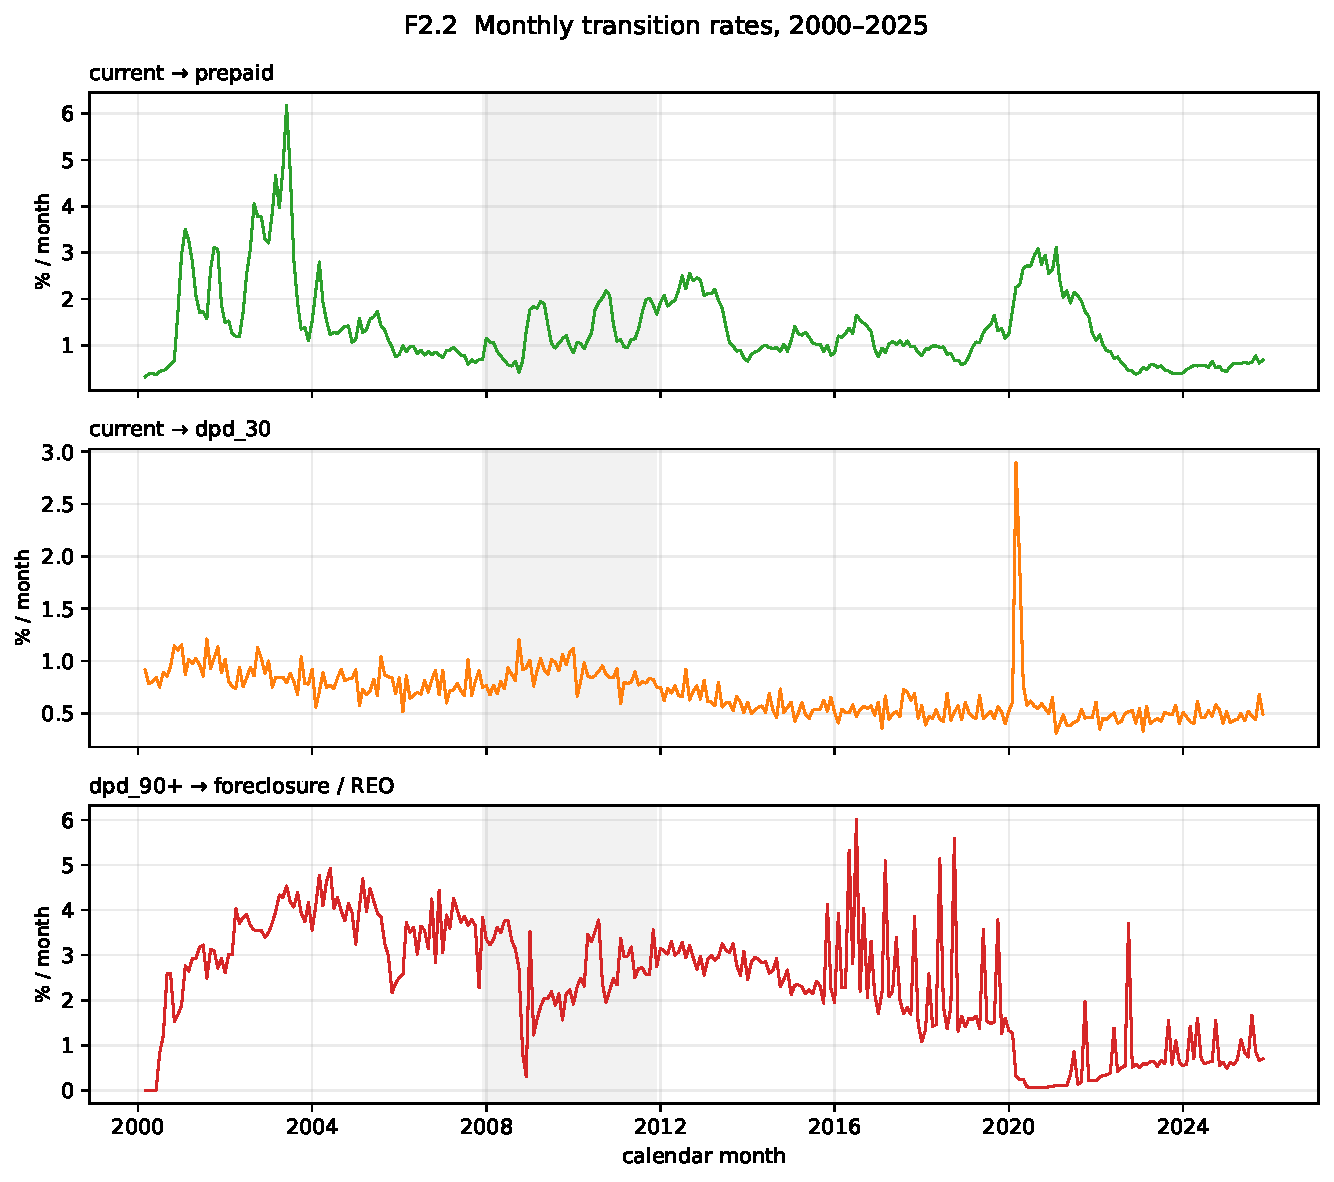
\includegraphics[width=0.9\textwidth]{figs/F2.2_transition_rates.pdf}
\caption[Monthly transition rates out of the Current state]{Monthly
transition rates out of the Current state, 2000--2025: prepayment and
entry into 30\,DPD (left axis), serious-delinquency terminations
(right axis).  Vertical shading marks the 2008--11 crisis and the
2020--21 forbearance episode.}\label{fig:transitionrates}
\end{figure}

\begin{table}[htbp]\centering\small
\caption[Summary statistics of model covariates]{Summary statistics of
the continuous model covariates over the full panel: null rate, mean,
standard deviation, and the min/1st/25th/50th/75th/99th/max
percentiles.}\label{tab:covariate-summary}
\resizebox{\textwidth}{!}{% Source: outputs/tables/eda/T1.2_covariate_summary_continuous.tex (full-panel
% Stage-6 QA). Tabular-only; wrap in \resizebox in chapter3.tex. Caption+label there.
\begin{tabular}{lrrrrrrrrrrl}
\toprule
column & null\_rate & mean & std & min & p01 & p25 & median & p75 & p99 & max & log\_flagged \\
\midrule
Original Interest Rate & 0 & 4.71882 & 1.32648 & 1.5 & 2.36602 & 3.62711 & 4.62688 & 5.75 & 7.85794 & 16.5 & False \\
Current Interest Rate & 0.012707 & 4.68763 & 1.32523 & 0 & 2.28982 & 3.625 & 4.60188 & 5.75 & 7.83746 & 13.5 & False \\
Original UPB & 0 & 199755 & 121639 & 1000 & 38809.4 & 109817 & 170562 & 262260 & 596156 & 2.326e+06 & True \\
Current Actual UPB & 0 & 159715 & 124113 & 0 & 0 & 71875.9 & 134287 & 224204 & 564970 & 2.86e+06 & True \\
Original Loan Term & 0 & 306.643 & 82.0617 & 36 & 120 & 202.959 & 360 & 360 & 360 & 360 & False \\
Loan Age & 0.01272 & 46.8107 & 42.4782 & -3 & 0 & 15 & 34.9747 & 65.8525 & 188.817 & 322 & False \\
Remaining Months to Maturity & 0.027474 & 252.795 & 97.4912 & 0 & 22.5446 & 167.472 & 294.279 & 335.84 & 359 & 480 & False \\
Original Loan-to-Value (LTV) & 0 & 69.7447 & 17.8489 & 1 & 21.1656 & 59.0522 & 74.5451 & 80 & 97 & 105 & False \\
Original Combined LTV (CLTV) & 0.003362 & 70.4277 & 17.9251 & 1 & 21.6837 & 59.7414 & 75 & 80 & 97 & 199 & False \\
Debt-to-Income (DTI) & 0.014108 & 33.3364 & 11.2275 & 0 & 9.02377 & 25 & 33.6755 & 41.9385 & 60.056 & 64 & False \\
fico\_orig & 0.002844 & 746.693 & 52.418 & 300 & 603.635 & 712.774 & 759.539 & 788.96 & 817.552 & 850 & False \\
fico\_co & 0.515382 & 754.702 & 49.6835 & 300 & 611.863 & 725.849 & 768.606 & 793.443 & 818.68 & 850 & False \\
Mortgage Insurance Percentage & 0.810875 & 24.1429 & 7.26184 & 0.12 & 6 & 22.29 & 25 & 30 & 35 & 50 & False \\
Number of Borrowers & 0.000119 & 1.55013 & 0.514524 & 1 & 1 & 1 & 2 & 2 & 2 & 10 & False \\
Number of Units & 0 & 1.03643 & 0.248099 & 1 & 1 & 1 & 1 & 1 & 2 & 4 & False \\
\bottomrule
\end{tabular}
}
\end{table}

% ────────────────────────────────────────────────────────────
\section{Exploratory Evidence: Nonlinearity and Interactions}
\label{sec:data-eda}

Before any model is fitted, the case that nonlinear modelling is
\emph{needed} can be made by counting alone.  The instrument is the
empirical hazard curve: bucket a covariate into equal-population
bins and plot the realised one-month transition rate per bin, with
Wilson 95\% confidence intervals.  Because each curve is a single
out-of-core aggregation over the columnar panel, the entire
programme runs in minutes.

\subsection{Single-covariate nonlinearity}
\label{subsec:data-eda-single}

Three hazard curves carry the argument.
\emph{Prepayment versus loan age}
(Figure~\ref{fig:hazard-age}): the rate rises from $0.27\%$ per month
at origination to a peak of $1.56\%$ at approximately 17 months of
age, then decays to $1.11\%$ by month 52 --- the classic
``seasoning hump,'' strongly non-monotone, with a secondary late-life
rise among long-surviving loans.  \emph{Prepayment versus the
refinancing incentive} (Figure~\ref{fig:hazard-incentive}): the rate
is flat at $0.4$--$0.6\%$ per month while the option is out of the
money, turns up sharply through zero, peaks at $2.71\%$ near
$+1.5$ percentage points of incentive, and falls back to $2.16\%$ by
$+2.7$ --- a roughly sevenfold range containing both an inflection
and a turning point, reproducing the flagship nonlinearity of
\citet{sirignano2021} on this cleaner credit box.
\emph{Delinquency versus credit score}
(Figure~\ref{fig:hazard-fico}): the entry rate into 30\,DPD falls
twenty-four-fold, from $3.06\%$ per month at FICO ${\approx}623$ to
$0.13\%$ at FICO ${\approx}815$, and the decay is convex --- the
slope in the low-score half is roughly $3.7$ times that in the
high-score half.  None of the three shapes is representable by a
linear term.

\begin{figure}[htbp]\centering
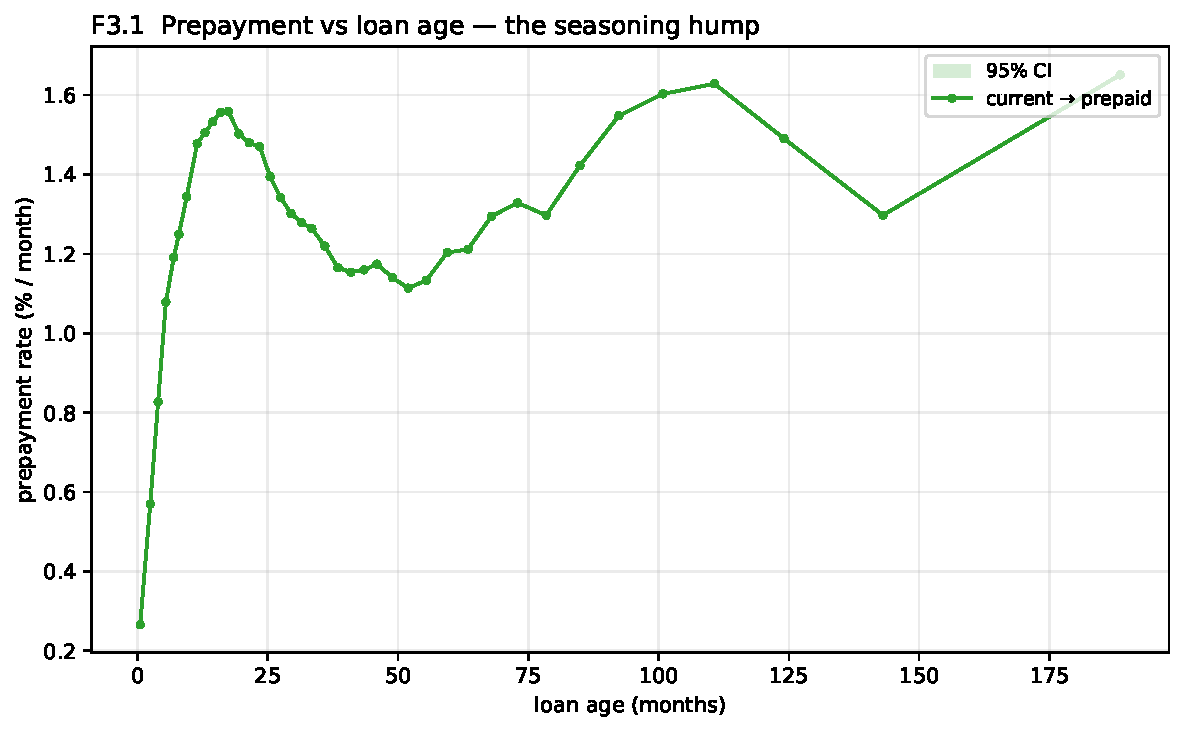
\includegraphics[width=0.8\textwidth]{figs/F3.1_prepay_age.pdf}
\caption[Empirical prepayment hazard by loan age]{Empirical prepayment
hazard by loan age (equal-population buckets, Wilson 95\% intervals):
the seasoning hump.}\label{fig:hazard-age}
\end{figure}

\begin{figure}[htbp]\centering
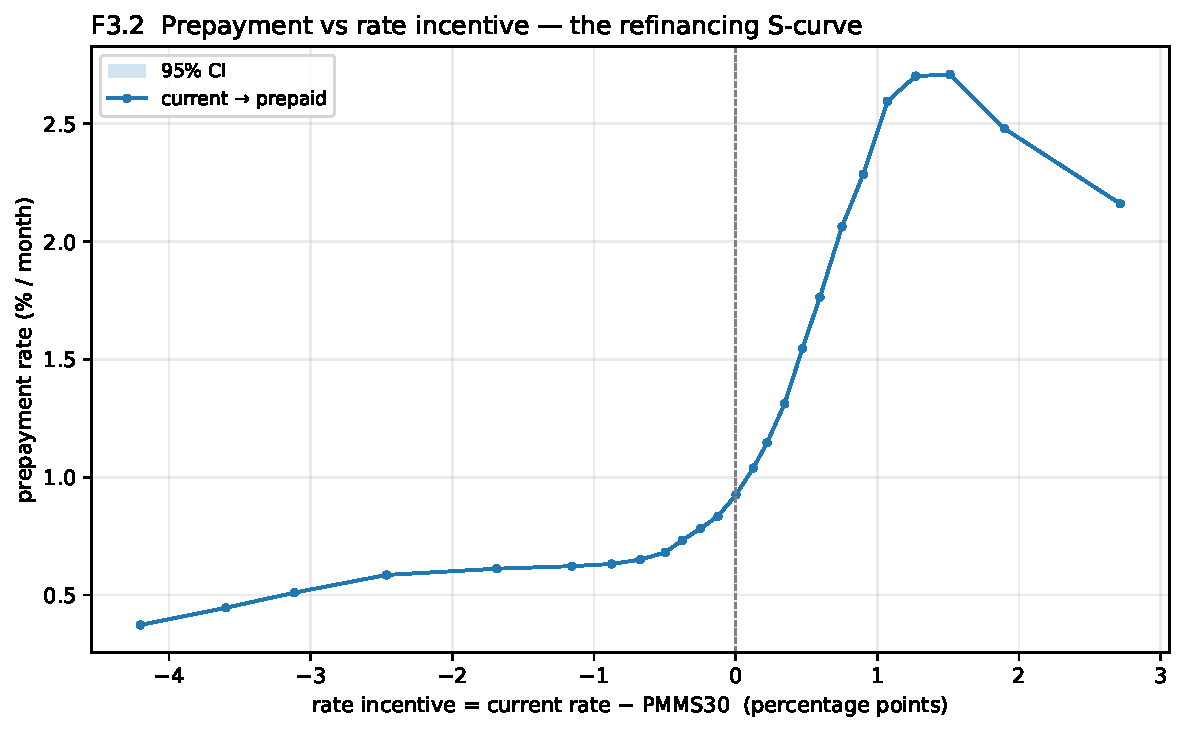
\includegraphics[width=0.8\textwidth]{figs/F3.2_prepay_incentive.pdf}
\caption[Empirical prepayment hazard by refinancing incentive]{Empirical
prepayment hazard by refinancing incentive: the S-curve, with burnout
beyond $+1.5$\,pp.}\label{fig:hazard-incentive}
\end{figure}

\begin{figure}[htbp]\centering
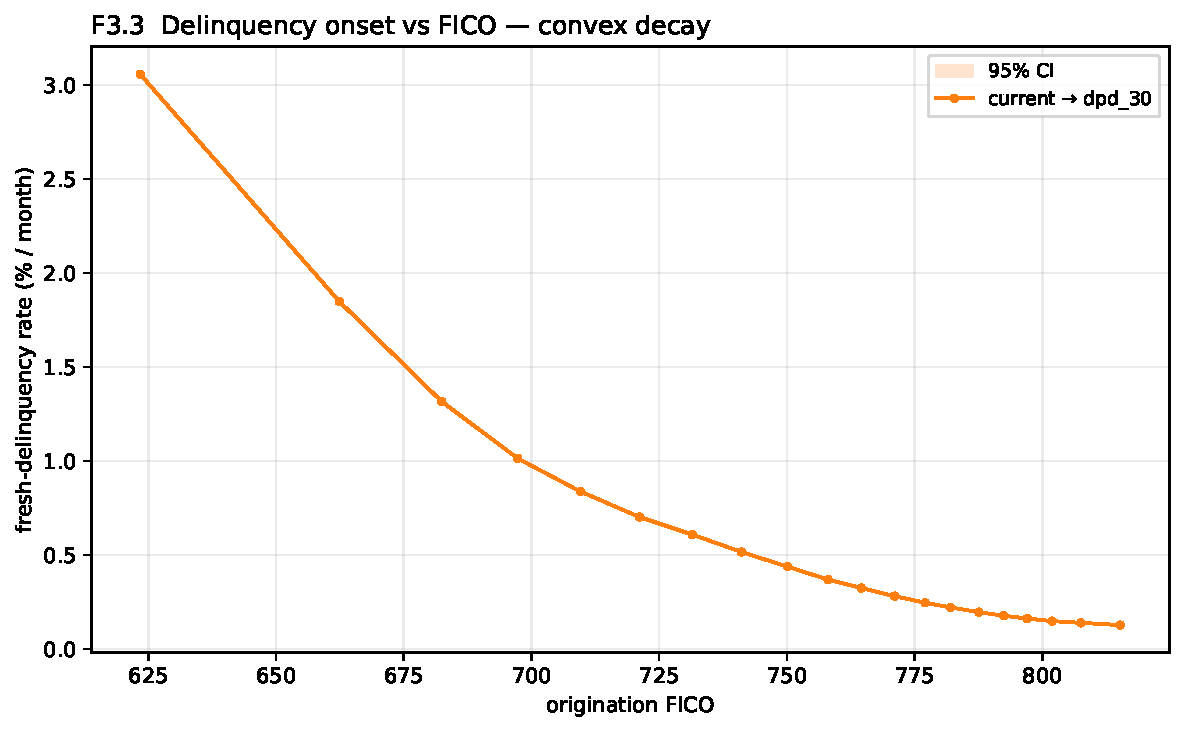
\includegraphics[width=0.8\textwidth]{figs/F3.3_delinq_fico.pdf}
\caption[Empirical 30\,DPD entry hazard by origination credit
score]{Empirical 30\,DPD entry hazard by origination credit score:
convex decay.}\label{fig:hazard-fico}
\end{figure}

\subsection{Interactions: the case against additivity}
\label{subsec:data-eda-interactions}

A linear-\emph{additive} model could in principle be patched with
transformed single-variable terms; interactions are what it cannot
absorb.  On a credit-score~$\times$~LTV grid
(Figure~\ref{fig:interaction-ficoltv}), the monthly rate of entry
into delinquency ranges from $0.11\%$ (best scores, lowest leverage)
to $2.69\%$ (worst scores, highest leverage) --- and decisively, the
\emph{additive} credit-score gradient (worst-minus-best rate) grows
from $1.73$ percentage points at low LTV to $2.48$ at high LTV, a
$43\%$ increase; equivalently, the leverage effect is roughly
$8.5$ times larger for low-score than high-score borrowers.
Additivity forces this gradient to be constant; the violation sits
exactly in the low-score/high-leverage corner that drives credit
losses.  In the prepayment channel
(Figure~\ref{fig:interaction-incfico}), splitting the incentive
S-curve by credit-score tercile shows the in-the-money refinancing
response \emph{rising} with credit quality --- $2.36\%$ per month in
the lowest tercile against $3.01\%$ in the highest --- because
credit-constrained borrowers cannot exercise the option: the
incentive \emph{slope} itself depends on the score.  Finally, holding
loan age fixed at 12--36 months to strip out seasoning, the
delinquency hazard by origination cohort isolates a clean vintage
effect: the 2007 cohort peaks at $1.68\%$ per month against $0.47\%$
for calm cohorts --- a $3.6$-fold premium
(Figure~\ref{fig:vintage}) --- so the origination vintage is a
feature in its own right, not reducible to contemporaneous
covariates.

\begin{figure}[htbp]\centering
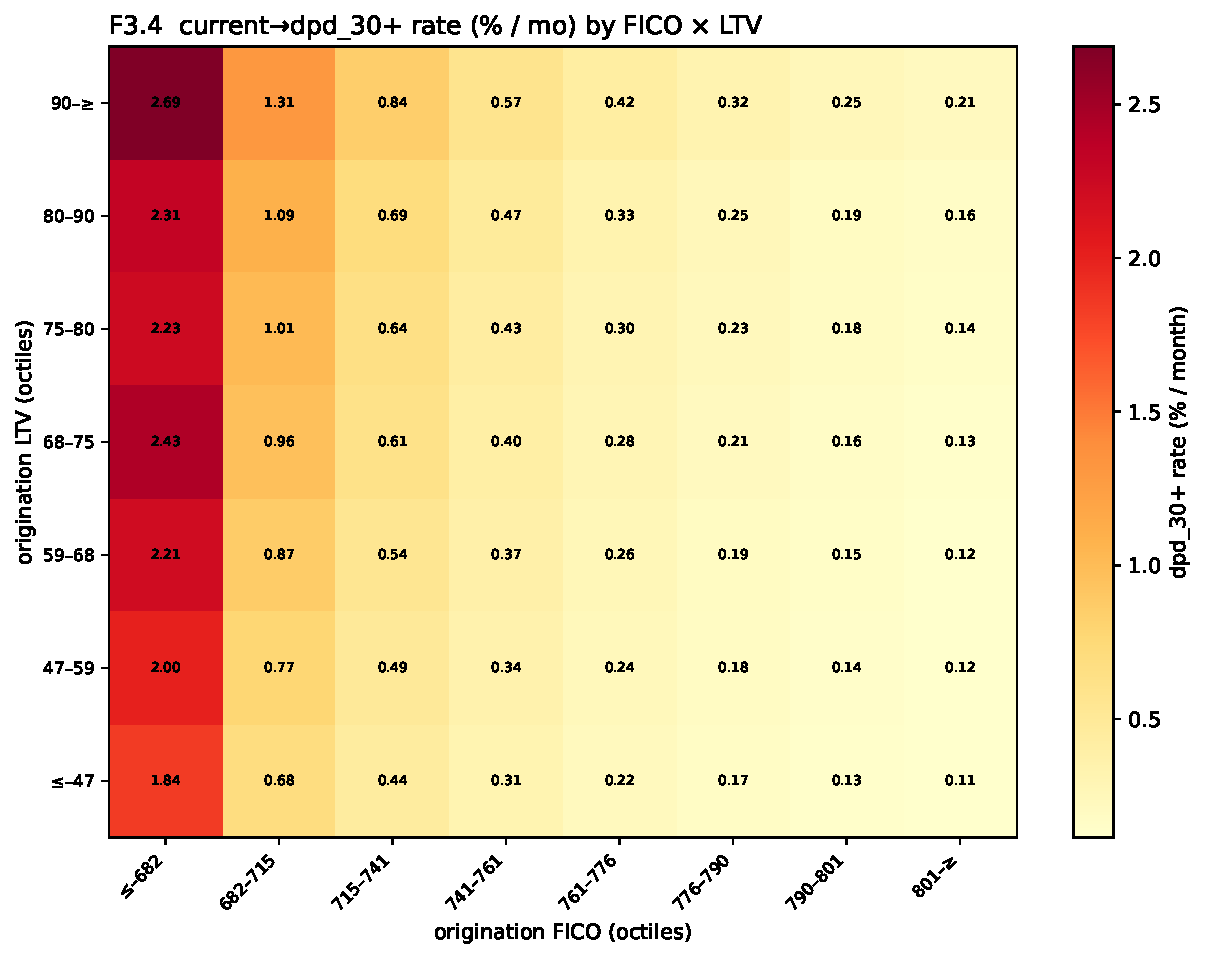
\includegraphics[width=0.78\textwidth]{figs/F3.4_fico_ltv_heatmap.pdf}
\caption[Monthly delinquency-entry rate on a credit-score $\times$ LTV
grid]{Monthly delinquency-entry rate on a credit-score $\times$ LTV grid
(equal-population bands): the additive credit-score gradient grows with
leverage --- additivity is misspecified.}\label{fig:interaction-ficoltv}
\end{figure}

\begin{figure}[htbp]\centering
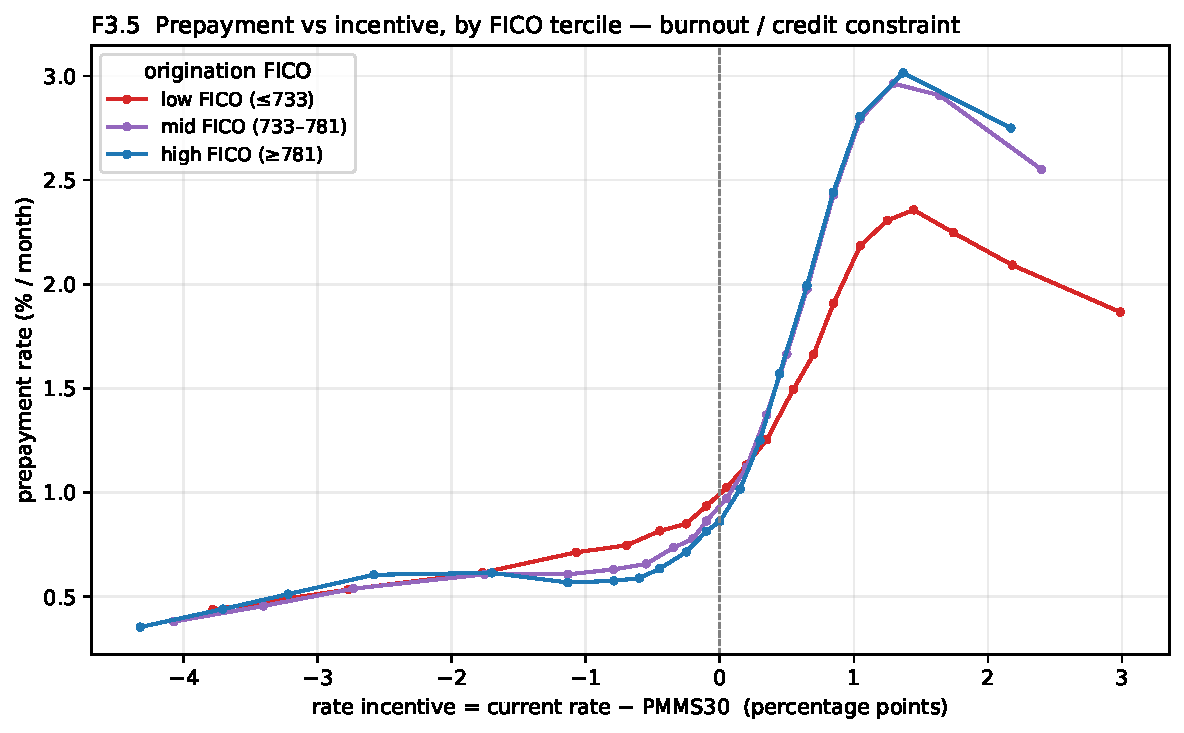
\includegraphics[width=0.8\textwidth]{figs/F3.5_incentive_fico.pdf}
\caption[The incentive S-curve by credit-score tercile]{The incentive
S-curve by credit-score tercile: the refinancing response to an
in-the-money option rises with credit
quality.}\label{fig:interaction-incfico}
\end{figure}

\begin{figure}[htbp]\centering
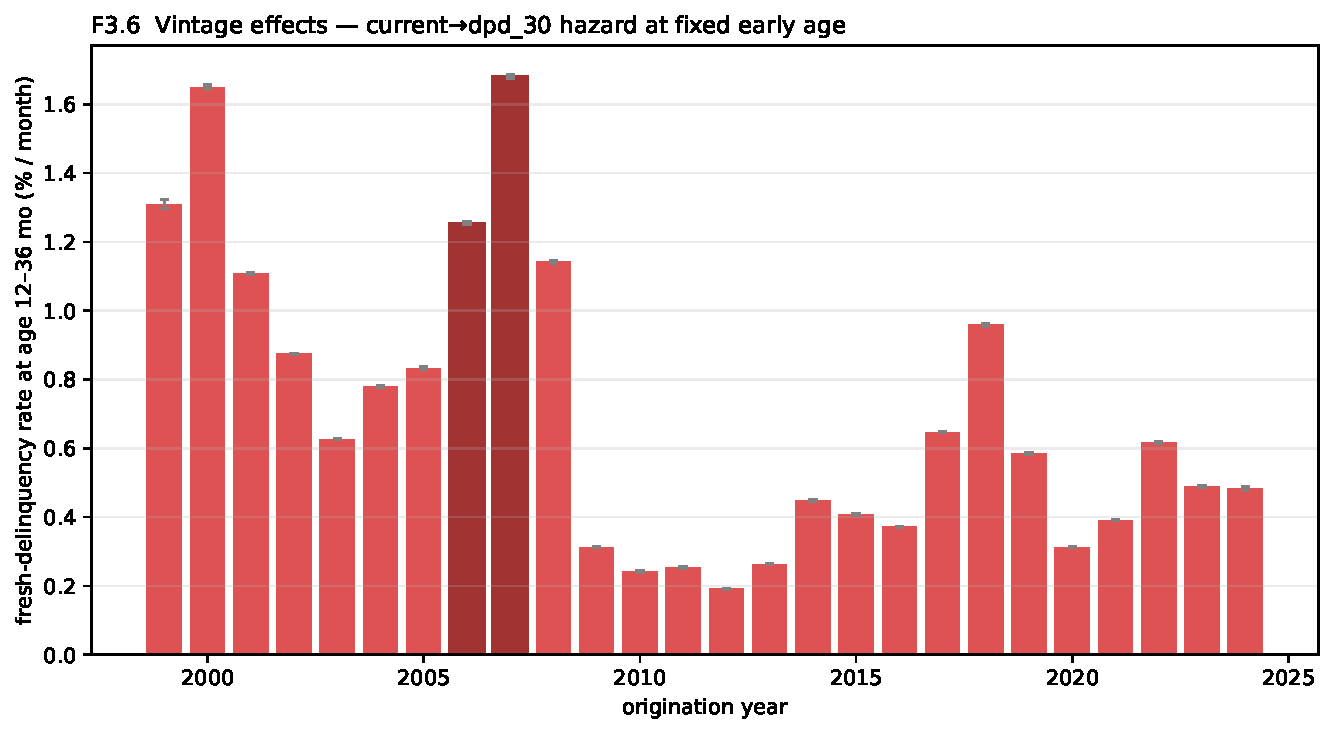
\includegraphics[width=0.8\textwidth]{figs/F3.6_vintage.pdf}
\caption[Delinquency hazard by origination cohort at fixed loan
age]{Delinquency hazard by origination cohort at fixed loan age
(12--36 months): the 2006--08 bubble vintages.}\label{fig:vintage}
\end{figure}

Taken together, the evidence points one way: monthly transition risk
depends on the covariates nonlinearly (the seasoning hump, the
incentive S-curve, convex credit-score decay) and interactively
(score$\times$leverage, incentive$\times$score, vintage).  A
linear-additive model should therefore underfit --- most severely on
prepayment, the channel combining the sharpest single-variable
nonlinearity with a first-order interaction --- and
Chapter~\ref{chap:results} tests precisely this.

% ────────────────────────────────────────────────────────────
\section{Comparison to Sirignano et al.\ (2021)}
\label{sec:data-comparison}

The dataset employed in the present study differs in several important
respects from the proprietary CoreLogic dataset used by
\citet{sirignano2021}, and these differences bear on the
interpretation of the results.

\citet{sirignano2021} draw on records for approximately 120 million
mortgages --- both prime and subprime --- originated across the United
States between January 1995 and June 2014, yielding approximately 3.5
billion loan-month observations.  The CoreLogic data encompass the
full spectrum of mortgage products, including fixed-rate,
adjustable-rate, hybrid, balloon, and interest-only loans, as well as
government-insured instruments.  Macro-economic covariates ---
zip-code-level house price indices from Zillow, county-level
unemployment rates from the Bureau of Labor Statistics, and the
Freddie Mac PMMS series --- are merged at the loan-month level within
the CoreLogic database.  The dataset is proprietary and cannot be
reproduced by independent researchers.

The Fannie Mae primary dataset, by contrast, is limited to
conventional fixed-rate fully-amortising loans and excludes both
subprime and government-insured products.  Macro-economic covariates
must be sourced and joined externally, as described in
Section~\ref{subsec:data-external}.  These differences have two
principal consequences.  First, the estimation sample is more
homogeneous in product mix; the nonlinear prepayment dynamics
associated with adjustable-rate burnout and subprime option exercise
--- prominent in \citeauthor{sirignano2021} --- are absent.  Second,
the absence of a subprime segment limits the range of credit-risk
outcomes observed; \citet{sirignano2021} report a median FICO score
of 630 for their subprime sub-sample against 730 for the prime
sub-sample, whereas the Fannie Mae population is concentrated at the
higher end of this credit-quality spectrum.

These limitations notwithstanding, the Fannie Mae dataset provides a
fully reproducible basis for the analysis.  The core methodological
contribution of \citet{sirignano2021} --- applying deep learning to a
multinomial competing-risks model of monthly loan-state transitions
--- transfers completely to the Fannie Mae panel.  The architecture,
estimation procedure, and evaluation framework described in subsequent
chapters are direct adaptations of that approach.  Table~\ref{tab:data-comparison}
summarises the key differences.

\begin{table}[htbp]
  \centering
  \small
  \begin{tabularx}{\textwidth}{@{} l X X @{}}
    \toprule
    \textbf{Dimension}
      & \textbf{Sirignano et al.\ (2021)}
      & \textbf{Present study} \\
    \midrule
    Data source
      & CoreLogic (proprietary)
      & Fannie Mae SFLP (public) \\[3pt]
    Total loans
      & ${\sim}120$ million
      & 57.6 million \\[3pt]
    Loan-month observations
      & ${\sim}3.5$ billion
      & 3.31 billion \\[3pt]
    Origination window
      & 1995--2014
      & 1999--2025 (full vintage set, reporting to 2025-12) \\[3pt]
    Products covered
      & Fixed, ARM, hybrid, balloon, IO
      & Fixed-rate, fully amortising only \\[3pt]
    Credit segments
      & Prime and subprime
      & Conventional (predominantly prime) \\[3pt]
    Macro covariates
      & Embedded (Zillow, BLS, PMMS)
      & External join required (FHFA HPI, PMMS) \\[3pt]
    Geographic detail
      & Full 5-digit zip code
      & 3-digit truncated zip; MSA \\[3pt]
    States modelled
      & Seven
      & Seven (identical mapping) \\[3pt]
    Reproducibility
      & Not publicly reproducible
      & Fully reproducible \\
    \bottomrule
  \end{tabularx}
  \caption[Comparison of the Fannie Mae SFLP dataset and the
  CoreLogic dataset used by Sirignano et al.\ (2021)]%
  {\textit{Comparison of the Fannie Mae SFLP primary dataset and the
  CoreLogic dataset used by \citet{sirignano2021}.}  CoreLogic counts
  are approximate as reported by the authors; Fannie Mae counts are
  measured on the assembled panel (Section~\ref{sec:data-summary}).}
  \label{tab:data-comparison}
\end{table}
          % Data & exploratory evidence
% ============================================================
%  Chapter 4 — Results
%  Status (M15c, June 2026): §4.1 (tuning window, tasks M7–M9 + M10b
%  depth check), §4.2 (rolling backtest + evaluation suite, M10b–M11),
%  and §4.3 (pool-level accuracy + economic translation, Phase 3
%  M13–M15) all carry real numbers and real artifacts from outputs/.
%  The four Phase-3 placeholders are swapped for F4.1 (fig:poolscatter),
%  T4.2 (tab:poolaccuracy), T5.1 (tab:econerrors), and F5.2
%  (fig:pricerrorbuckets); .tex tables regenerate via
%  dev/model/make_pool_tex.py from the committed M14/M15b JSON. All
%  numbers/tables/figures trace to outputs/{tables,figures}/{loan,pool}_level.
% ============================================================

\chapter{Results}
\label{chap:results}

All results in this chapter are out of sample under the rolling
design of Section~\ref{sec:meth-design} unless explicitly labelled
in-sample.  Negative log-likelihood (NLL) is reported as the mean of
\eqref{eq:nll} over the relevant frozen test rows; lower is better.

\section{Architecture selection and benchmarks on the tuning window}
\label{sec:results-tuning}

Hyperparameter and architecture selection was carried out once, on
the $k{=}2015$ tuning window (training on labels through December
2013, early stopping and selection on validation year 2014), and
frozen thereafter.  The search covered depth
$L\in\{1,3,5,7\}$ $\times$ dropout $\{0, 0.2, 0.5\}$ at zero weight
decay, plus an $\ell_2$ sweep at the five-layer anchor --- a
pruned grid of 14 cells anchored at the five-layer geometry of
\citet{sirignano2021}.

\begin{table}[htbp]\centering\small
\caption[Tuning-window architecture comparison (analogue of
\citealp{sirignano2021} Table 11)]{Tuning-window comparison (the
analogue of Table 11 in \citealp{sirignano2021}): in- and
out-of-sample NLL on the $k{=}2015$ window (dev export) for the
empirical matrix, bucketed matrix, multinomial logit, augmented logit,
neural networks of depth 1/3/5/7, the selected configuration with
dropout, and the eight-network ensemble.  Frequency benchmarks and the
augmented logit carry no in-sample column.}\label{tab:tablea}
% Source: outputs/tables/loan_level/table_a.tex (k=2015 dev export).
% Tabular-only; Unicode sanitized for OT1/pdfLaTeX. Caption+label in chapter4.tex.
\begin{tabular}{lrr}
\toprule
Model & In-sample NLL & Out-of-sample NLL \\
\midrule
Empirical matrix & --- & 0.112661 \\
Bucketed matrix & --- & 0.109247 \\
Logit & 0.141395 & 0.109430 \\
Augmented logit & --- & 0.108843 \\
NN depth 1 (no reg) & 0.136005 & 0.103680 \\
NN depth 3 (no reg) & 0.135114 & 0.104159 \\
NN depth 5 (no reg) & 0.134329 & 0.104299 \\
NN depth 7 (no reg) & 0.134434 & 0.104176 \\
NN-5 + dropout 0.2 & 0.136880 & 0.104845 \\
NN best single ($L{=}3$, dropout 0.2) & 0.133948 & 0.103187 \\
Ensemble $\times 8$ ($L{=}3$, dropout 0.2) & 0.134417 & 0.102741 \\
\bottomrule
\end{tabular}

\end{table}

Three findings from the grid, at dev scale (a stratified
$\sim$3.15-million-row training slice of the window):

\begin{itemize}
\item \textbf{Regularisation moves the optimum deeper.}  Without
  dropout the validation-optimal depth is one hidden layer; with
  dropout $0.2$ it shifts to three --- qualitatively replicating the
  dropout--depth interaction documented by \citet{sirignano2021}.  A
  small $\ell_2$ penalty ($10^{-5}$) partially rescues the five-layer
  network (validation NLL $0.09767 \to 0.09630$) but does not
  overturn the ordering.
\item \textbf{The selected configuration} is depth 3, dropout
  $0.2$: validation NLL $0.09602$, test NLL $0.10319$ on the tuning
  window.  In-sample NLL exceeding out-of-sample in parts of the grid
  is expected here, not inverted overfitting: the expanding training
  window (2000--2013) contains the crisis years while the 2015 test
  year is calm.
\item \textbf{The ensemble helps, with diminishing returns.}  The
  eight-network ensemble at the selected configuration reaches test
  NLL $0.10274$, beating both the average single member ($0.10359$)
  and the best individual member ($0.10307$); the ensemble-size curve
  flattens by roughly five members
  (Figure~\ref{fig:ensemblecurve}).
\end{itemize}

\begin{figure}[htbp]\centering
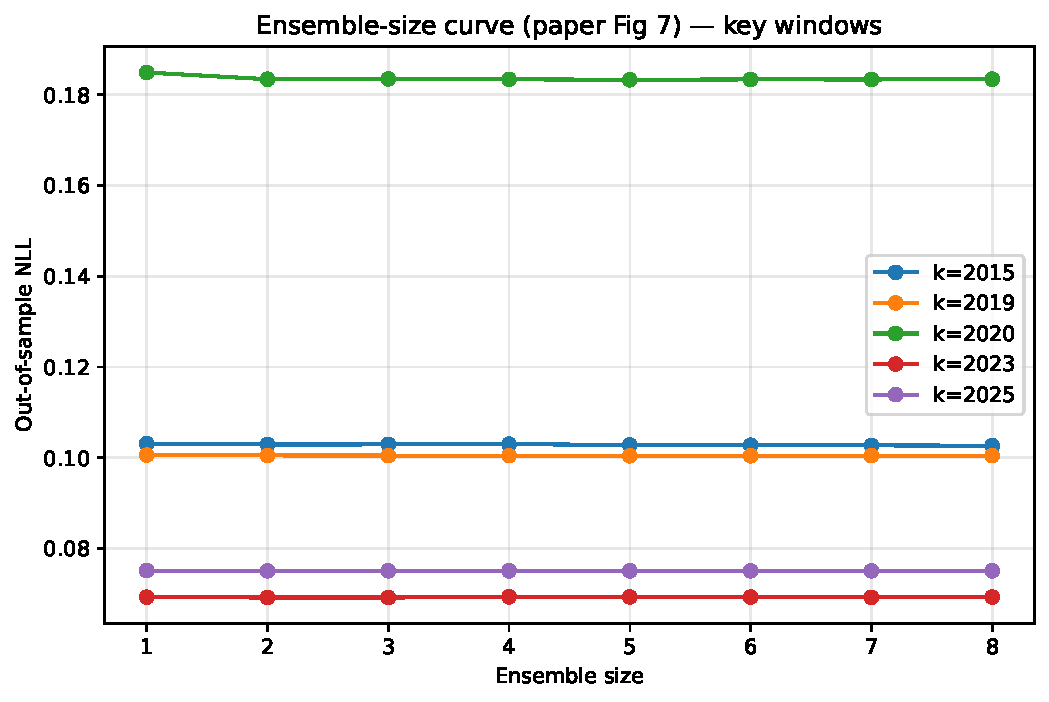
\includegraphics[width=0.8\textwidth]{figs/F_ensemble_size_curve.pdf}
\caption[Out-of-sample NLL versus ensemble size, tuning window]{Out-of-sample
NLL versus number of ensemble members, tuning window (the analogue of
Figure 7 in \citealp{sirignano2021}).}\label{fig:ensemblecurve}
\end{figure}

The multinomial logit baseline was validated against a standard
library implementation (agreement in NLL to within $10^{-3}$ across
the regularisation grid; the loop's embedding-based reimplementation
subsequently matched it to within $10^{-4}$), so the gaps between
logit and network rows in Table~\ref{tab:tablea} are attributable to
architecture alone.

\paragraph{Full-scale depth check.}  Because the grid above was run
at dev scale, the depth choice was re-examined at full scale
($\sim$33.5 million training rows, $10.6\times$ the dev slice) before
the rolling loop was launched: depth 3 and depth 5 were re-fitted on
the full tuning window (with and without the $\ell_2$ rescue).  Depth
3 won robustly on validation (its best validation NLL $0.09572$
against depth 5's $0.09591$), and the frozen configuration for the
loop is depth 3, dropout $0.2$, weight decay $10^{-5}$.  This is a substantive deviation from
\citet{sirignano2021}, whose optimum at population scale was five
layers: on the prime conforming credit box, the optimal network is
\emph{shallower} --- the nonlinearity premium documented in
Section~\ref{sec:data-eda} is real but structurally simpler than in
subprime-heavy private-label data.
%RESULTS-DEPENDENT: revisit wording after M12 (seed variance,
%tuning-window sensitivity on k=2019) to state robustness precisely.

\section{The rolling backtest, 2015--2025}
\label{sec:results-rolling}

The frozen configuration of Section~\ref{sec:results-tuning} --- depth
3, dropout $0.2$, weight decay $10^{-5}$ --- is refitted from scratch
on each of the eleven rolling windows (per-window scaler, embedding
vocabulary, and rate incentive; early stopping on that window's
validation year), alongside a per-window multinomial logit and, on the
five regime-spanning key windows $\{2015, 2019, 2020, 2023, 2025\}$,
an eight-network ensemble.  Every model is scored on the same frozen,
unthinned test slice for its window, so each of the 84.5\,million
pooled test rows is predicted exactly once by a model that never saw
it.

Table~\ref{tab:tableb} is the headline exhibit: out-of-sample NLL by
test year, with the pooled all-years comparison and the by-origin-state
breakdown beneath.  \textbf{The network beats the logit in every one of
the eleven test years} --- calm years, the 2020 COVID forbearance
spike, and the 2022--23 rate shock alike
(Figure~\ref{fig:nllbyyear}).  Pooled over all 84.5\,million test rows,
NLL falls from the $0.111477$ covariate-free empirical floor to
$0.108249$ for the logit and $0.101468$ for the network: the logit
recovers only $2.9\%$ of the distance below the floor while the network
recovers $9.0\%$, so the nonlinearity supplies roughly two-thirds of
the achievable improvement.  The 2020 window is by far the hardest for
every model (NLL ${\approx}\,0.18$--$0.19$, about twice the calm-year
level), reflecting the forbearance-driven distribution shift in the
delinquency codes; the network's relative edge over the logit
nonetheless holds there too.

Because the ensemble was fit only on the five key windows, it is
\emph{not} pooled into the all-years figure --- doing so would compare
it against the logit and network on a different, COVID-weighted set of
rows.  It is read against the network per window instead, in the five
key-year rows of Table~\ref{tab:tableb}: the ensemble's test NLL is at
or below the deployed single network in four of the five (2015, 2019,
2020, 2025) and ties within seed noise on 2023
($+2.2\times10^{-5}$) --- the small variance-reduction effect of
\citeauthor{sirignano2021}'s Figure 7, muted on this cleaner credit
box.

\begin{table}[htbp]\centering\small
\caption[Rolling out-of-sample NLL by test year and origin
state]{Out-of-sample NLL by test year and model, 2015--2025 (top),
with the pooled all-years comparison, and the pooled-NLL breakdown by
origin state (bottom).  Pooled figures are over all eleven windows
(84.5\,M test rows); the eight-network ensemble was fit only on the
five key windows and is therefore reported per year, not pooled --- a
pooled-all-years ensemble figure would mix incomparable row
coverage.}\label{tab:tableb}
% Source: outputs/tables/loan_level/table_b.tex (full export, frozen test slices).
% Tabular-only; Unicode sanitized. The pooled column is restricted to the models
% that exist on all eleven windows (empirical, logit, network): the 8-net ensemble
% was fit only on the five key windows, so a pooled-all-years ensemble figure would
% mix incomparable row coverage and is shown ``---''. The ensemble is compared to
% the network per window in the five key-year rows above. Caption+label in chapter4.tex.
\begin{tabular}{lrrrr}
\toprule
Test year & Empirical matrix & Logit & Best NN & Ensemble $\times 8$ \\
\midrule
2015 & 0.112870 & 0.108246 & 0.103125 & 0.102662 \\
2016 & 0.119296 & 0.116390 & 0.109378 & --- \\
2017 & 0.108116 & 0.105750 & 0.097431 & --- \\
2018 & 0.099608 & 0.098172 & 0.088404 & --- \\
2019 & 0.109673 & 0.106352 & 0.100600 & 0.100479 \\
2020 & 0.193580 & 0.191949 & 0.184869 & 0.183414 \\
2021 & 0.153786 & 0.149628 & 0.141729 & --- \\
2022 & 0.093759 & 0.090422 & 0.085874 & --- \\
2023 & 0.079130 & 0.074943 & 0.069296 & 0.069318 \\
2024 & 0.082829 & 0.079053 & 0.072203 & --- \\
2025 & 0.085575 & 0.082164 & 0.075157 & 0.075095 \\
\midrule
\textbf{Pooled (11 windows)} & 0.111477 & 0.108249 & 0.101468 & --- \\
\bottomrule
\end{tabular}


\vspace{1.5ex}
% Source: outputs/tables/loan_level/table_b.* (pooled NLL by origin state, all 11
% windows, 84.5 M test rows). Ensemble omitted: it exists only on the five key
% windows, so a pooled-all-years ensemble column would mix row coverage.
\begin{tabular}{lrrrr}
\toprule
Origin state & $n$ (rows) & Empirical & Logit & Best NN \\
\midrule
Current   & 82{,}817{,}018 & 0.094731 & 0.091067 & 0.085066 \\
30\,DPD   &    788{,}362 & 1.117058 & 1.147346 & 1.090599 \\
60\,DPD   &    220{,}753 & 1.360988 & 1.387931 & 1.335079 \\
90+\,DPD  &    686{,}244 & 0.575219 & 0.576468 & 0.547682 \\
\bottomrule
\end{tabular}

\end{table}

\begin{figure}[htbp]\centering
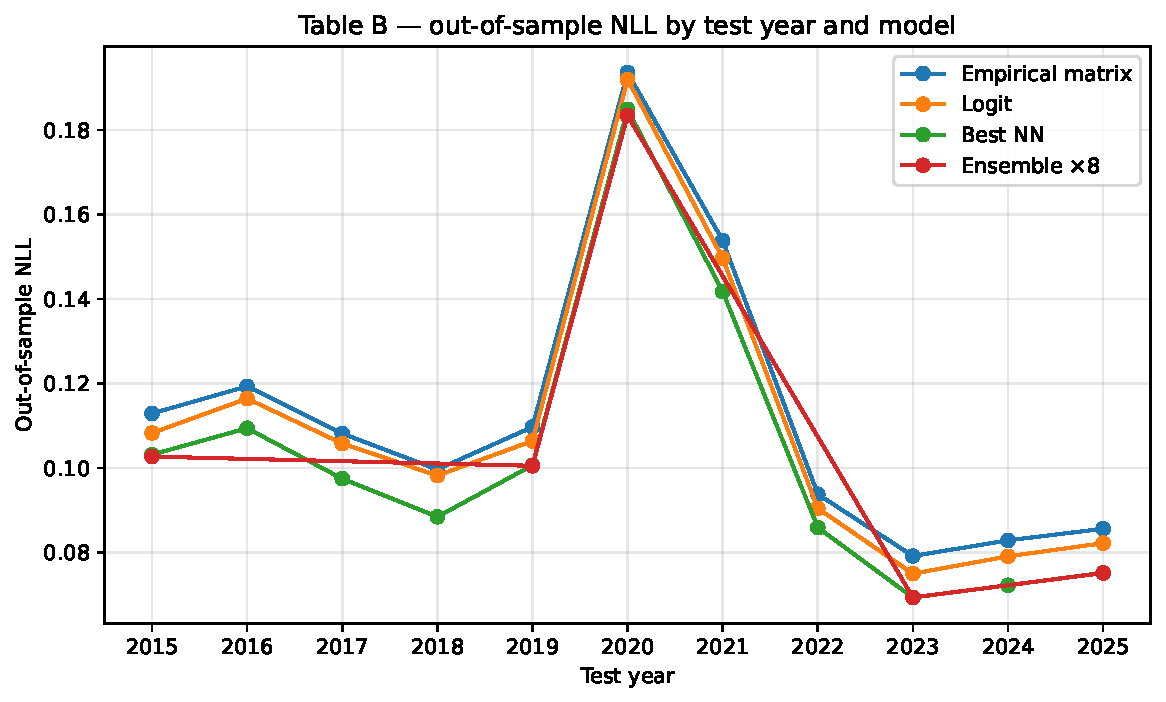
\includegraphics[width=0.85\textwidth]{figs/F_tableB_nll_by_year.pdf}
\caption[Out-of-sample NLL by test year, one line per model]{Out-of-sample
NLL by test year, one line per model: the time series of the value of
nonlinearity.  The ensemble line is drawn only on the five key
windows.}\label{fig:nllbyyear}
\end{figure}

The discrimination gain concentrates exactly where the exploratory
evidence of Section~\ref{sec:data-eda} located the nonlinearity.
Table~\ref{tab:auc} reports one-versus-rest AUC by origin and
destination, pooled over all eleven windows for the two models that
span them.  The network's largest edges are in the prepayment channel
(Current$\to$Prepaid AUC $0.653 \to 0.748$), which combines the
sharpest single-variable nonlinearity with a first-order interaction
with credit, and in the deep-delinquency transitions the logit cannot
even rank (90+\,DPD$\to$Foreclosure $0.482 \to 0.623$, from below
chance to a genuine ranker).  On the five key windows the ensemble's
AUC is at or above the single network's in nearly every cell,
consistent with its marginal NLL gain.

\begin{table}[htbp]\centering\small
\caption[One-versus-rest AUC by transition, all eleven windows
pooled]{One-versus-rest AUC by origin and destination state, pooled
over all eleven windows of test predictions (84.5\,M rows): logit
versus network.  Restricted to the two models fit on every window; the
ensemble (five key windows only) is discussed in the
text.}\label{tab:auc}
% Source: outputs/tables/loan_level/auc.* -- ALL ELEVEN WINDOWS pooled
% (84.5 M test rows), logit vs network. This is the pooled all-years comparison and
% is therefore restricted to the two models that exist on every window. The 8-net
% ensemble (five key windows only) is compared to the network on its matched windows
% in the text. Tabular-only; caption+label in chapter4.tex.
\begin{tabular}{llrrr}
\toprule
Origin & Destination & $n_{+}$ & Logit & Network \\
\midrule
Current  & Current      & 81{,}466{,}577 & 0.6538 & 0.7225 \\
Current  & 30\,DPD      &    438{,}665 & 0.7639 & 0.7684 \\
Current  & Prepaid      &    908{,}017 & 0.6527 & 0.7484 \\
30\,DPD  & Current      &    321{,}129 & 0.6098 & 0.6264 \\
30\,DPD  & 30\,DPD      &    312{,}451 & 0.6152 & 0.6266 \\
30\,DPD  & 60\,DPD      &    141{,}904 & 0.5320 & 0.5322 \\
30\,DPD  & Prepaid      &     11{,}764 & 0.5899 & 0.6659 \\
60\,DPD  & Current      &     33{,}750 & 0.5726 & 0.5883 \\
60\,DPD  & 30\,DPD      &     30{,}105 & 0.5961 & 0.6034 \\
60\,DPD  & 60\,DPD      &     66{,}512 & 0.5590 & 0.5614 \\
60\,DPD  & 90+\,DPD     &     87{,}182 & 0.5481 & 0.5939 \\
60\,DPD  & Prepaid      &      3{,}190 & 0.5559 & 0.6198 \\
90+\,DPD & Current      &     56{,}883 & 0.5890 & 0.6021 \\
90+\,DPD & 30\,DPD      &      7{,}482 & 0.5405 & 0.6294 \\
90+\,DPD & 60\,DPD      &     10{,}519 & 0.5687 & 0.6630 \\
90+\,DPD & 90+\,DPD     &    594{,}879 & 0.5465 & 0.5717 \\
90+\,DPD & Foreclosure  &      4{,}257 & 0.4818 & 0.6233 \\
90+\,DPD & Prepaid      &      8{,}747 & 0.5434 & 0.6257 \\
\bottomrule
\end{tabular}

\end{table}

The aggregate fit is examined two ways.
Figure~\ref{fig:calibration} gives reliability diagrams for the two
dominant Current transitions, pooled and split out for the 2020--21
forbearance years: the network tracks the diagonal markedly better than
the logit, whose miscalibration is worst in the high-hazard upper bins
(the burned-out, deep-in-the-money tail of the prepayment S-curve).
Both models degrade under the 2020--21 shift, but the network remains
the better-calibrated of the two.  Figure~\ref{fig:rateoverlay}
overlays predicted and realised \emph{monthly aggregate} transition
rates over 2015--2025: the network reproduces the level and the timing
of the prepayment waves and the 2022--23 collapse, with the realised
2020 delinquency spike the one place the aggregate prediction lags ---
the expected forbearance-shock miss.

\begin{figure}[htbp]\centering
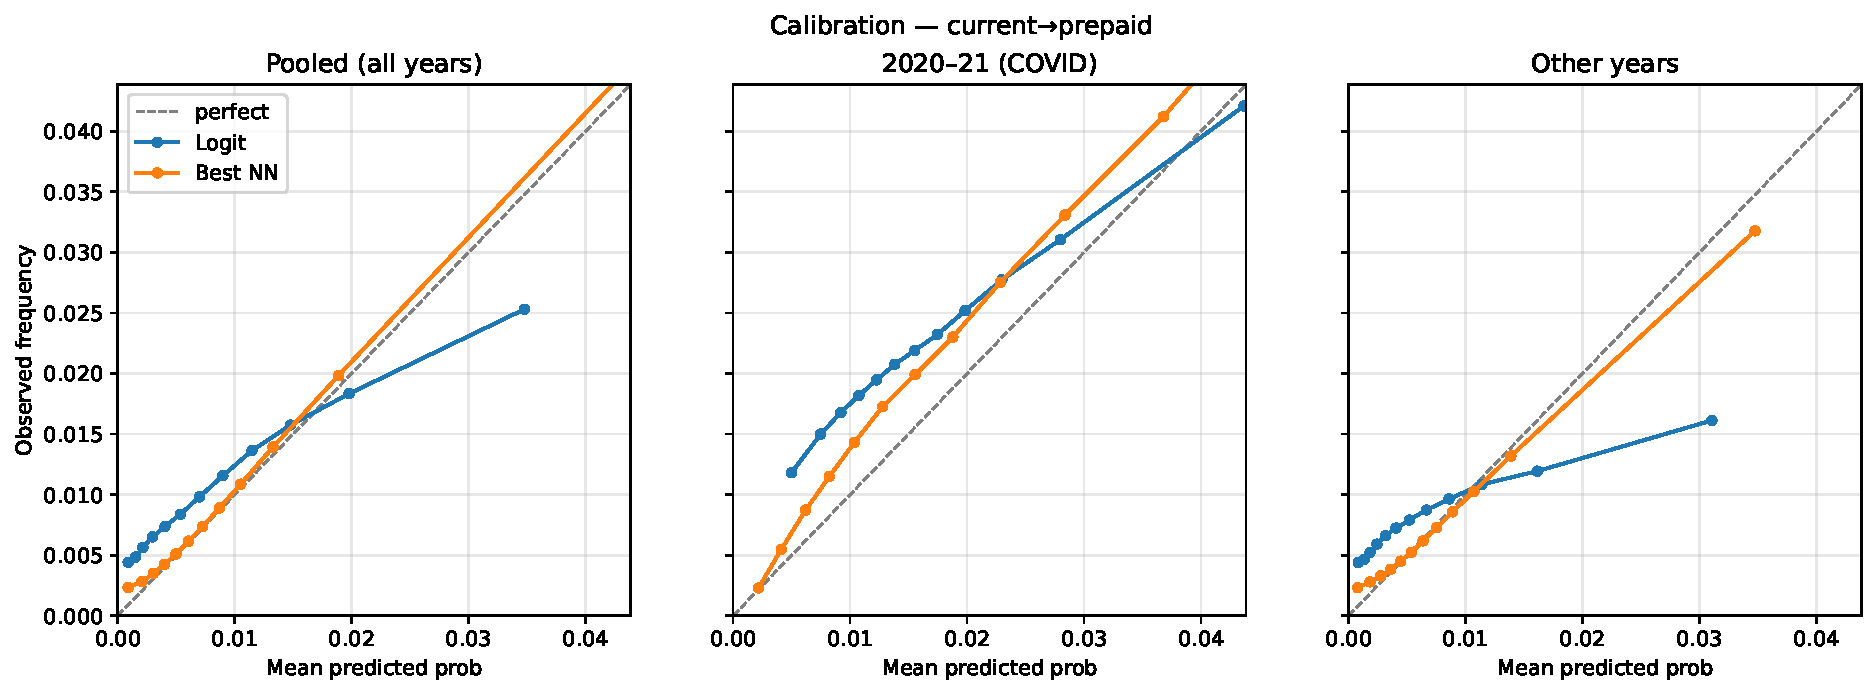
\includegraphics[width=0.49\textwidth]{figs/F_calibration_current_to_prepaid.pdf}\hfill
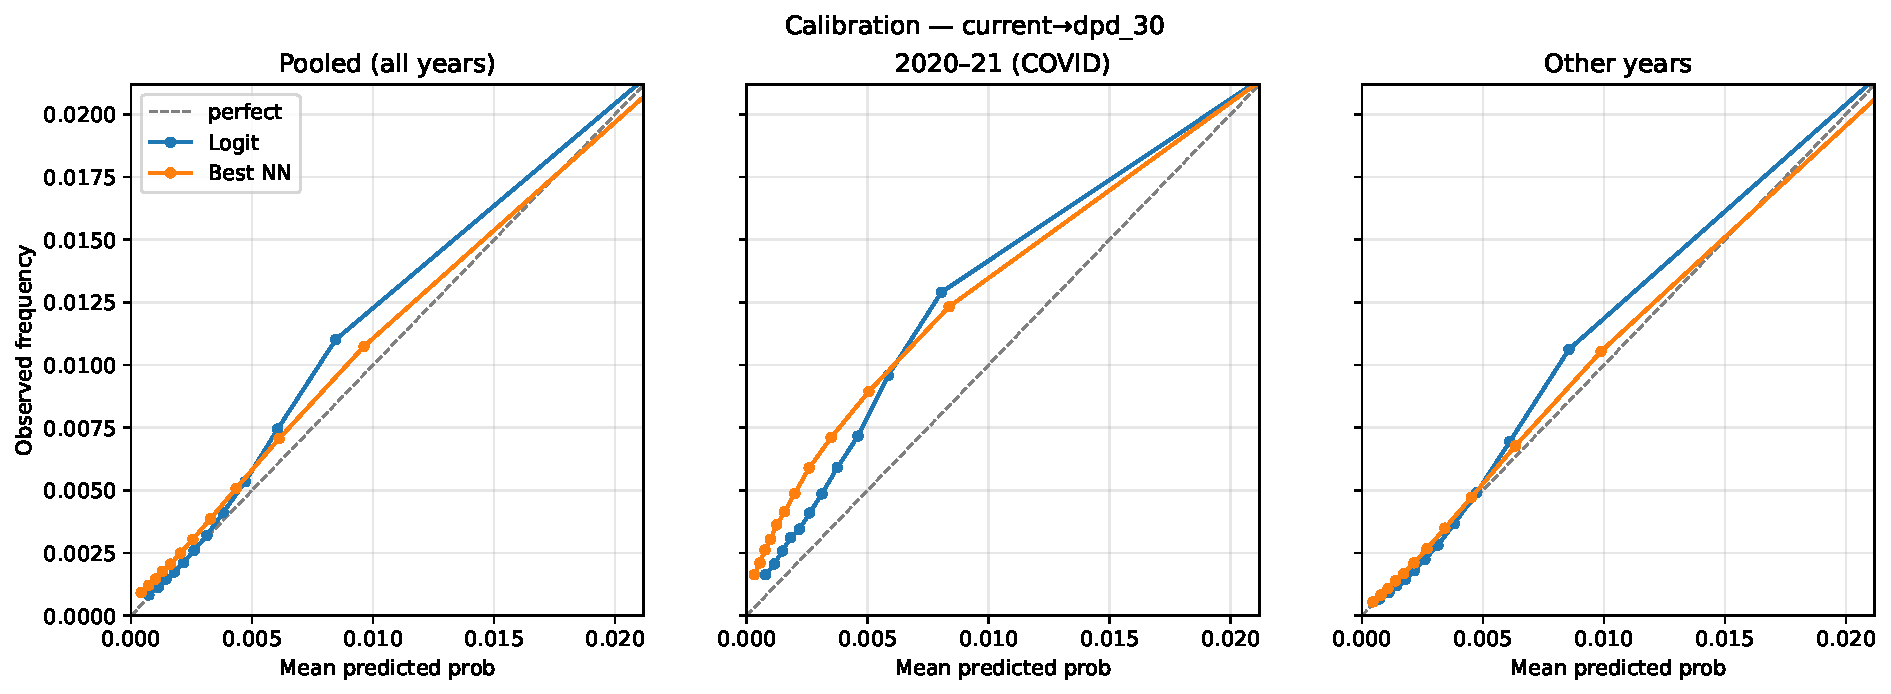
\includegraphics[width=0.49\textwidth]{figs/F_calibration_current_to_dpd_30.pdf}
\caption[Reliability diagrams, Current transitions]{Reliability
diagrams for the Current$\to$Prepaid (left) and Current$\to$30\,DPD
(right) transitions, pooled and for the 2020--21 forbearance years
separately: the network is the better-calibrated of the two
models.}\label{fig:calibration}
\end{figure}

\begin{figure}[htbp]\centering
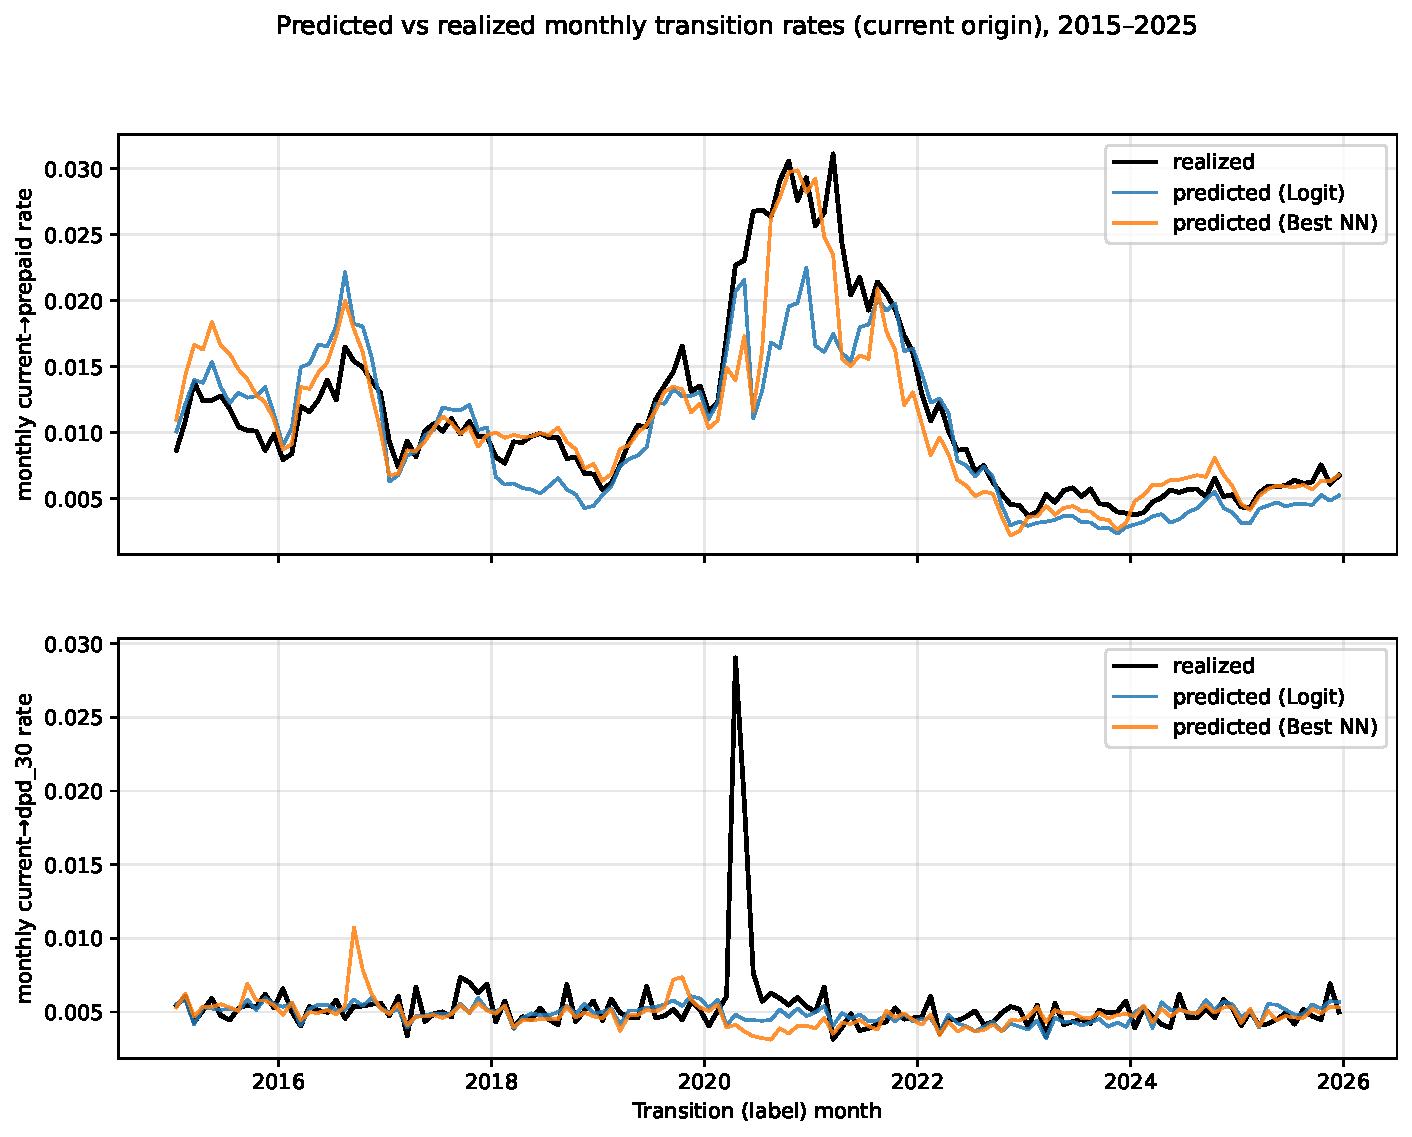
\includegraphics[width=0.85\textwidth]{figs/F_rate_overlay.pdf}
\caption[Predicted versus realised aggregate transition rates]{Predicted
versus realised monthly aggregate Current$\to$Prepaid and
Current$\to$30\,DPD transition rates, 2015--2025.}\label{fig:rateoverlay}
\end{figure}

Robustness exhibits: seed variance of the selected network against the
network--logit gap; stability of the model ranking across the eleven
test years (notably through 2020--21 and 2022--23); re-tuning
sensitivity on the $k{=}2019$ window; and the width sweep at the
selected configuration (Appendix~\ref{app:supplementary}).

\section{Pool-level results and economic translation}
\label{sec:results-pool}

The loan-level models of Section~\ref{sec:results-rolling} are now
aggregated to pools by the roll-forward of
Section~\ref{subsec:meth-pools}: for every loan alive at a window
anchor $t_0{=}\text{Dec}(k{-}1)$, the window-$k$ model's monthly
transition matrices are composed twelve steps forward to a horizon
event probability, and pool counts and speed paths follow from
\eqref{eq:poolcount} and Section~\ref{subsec:meth-econ}.  Only the
deterministic covariates evolve along the chain (loan age, remaining
term, calendar seasonality); the entire macroeconomic block --- rate
incentive, unemployment, house-price growth --- is \emph{frozen at the
anchor}, so every prediction is conditional on the $t_0$ environment.
Five regime-spanning anchors are scored, each with its own frozen
window-$k$ models: Dec2014 (calm), Dec2018 (late cycle), Dec2019
(entering the COVID forbearance shock), Dec2022 (the rate spike), and
Dec2024.

\subsection{Pool-level accuracy and the regime exhibit}

Figure~\ref{fig:poolscatter} is the flagship pool exhibit:
predicted versus realised twelve-month prepayment counts for the 500
random pools at Dec2024, one panel per model.  The improvement in
\emph{level} is stark --- the covariate-free empirical matrix predicts
roughly $2.5\times$ too many prepayments (its flat CPR floor ignores
that the 2024 cohort is deeply out of the money), the logit closes most
of the gap, and the ensemble cloud sits nearest the diagonal (RMSE
$82.9 \to 28.0 \to 11.9$ loans).  The $R^2$ values are all negative
even for the ensemble: random pools are near-homogeneous $1{,}000$-loan
draws, so cross-pool realised variance is tiny and $R^2$ is dominated
by a small level bias --- the random scheme tests \emph{level}
calibration, not cross-pool discrimination, which is why the
discriminating metric is read from the characteristic buckets instead.

Table~\ref{tab:poolaccuracy} gives that characteristic-bucket panel ---
$R^2$ and RMSE by model, outcome, and anchor --- and it is the regime
exhibit promised in Section~\ref{sec:intro-contributions}: a time
series of the value of nonlinearity, not a single verdict.
\textbf{Which model prices a pool best depends on whether the shock
lands in a covariate-captured channel.}  In calm and late-cycle
regimes the covariate models dominate (Dec2014 prepaid $R^2$
$0.58/0.98/0.98$ for empirical/logit/ensemble).  Under the
\emph{rate/prepayment-incentive shock} of 2022--24 --- precisely the
channel the rate-incentive covariates encode --- the empirical matrix
collapses to large negative $R^2$ ($-4.62$ at Dec2022, $-1.46$ at
Dec2024) while the ensemble is strongest ($0.85$, $0.94$; RMSE $415$
against the logit's $991$ at Dec2024).  But under the 2020
\emph{forbearance/credit shock} the ordering \emph{inverts}: at Dec2019
the assumption-free empirical floor is best ($R^2\,0.65$) and the
ensemble is worst ($0.45$), because the ensemble bakes in hardest a
pre-COVID prepayment signal that March 2020 abruptly invalidates.  For
the rare serious-delinquency outcome RMSE is the reliable metric (with
$\sim$16 buckets $R^2$ is unstable across all models), and the ensemble
is the only model with positive $60{+}$\,DPD $R^2$ at the 2022 and 2024
anchors.

\begin{figure}[htbp]\centering
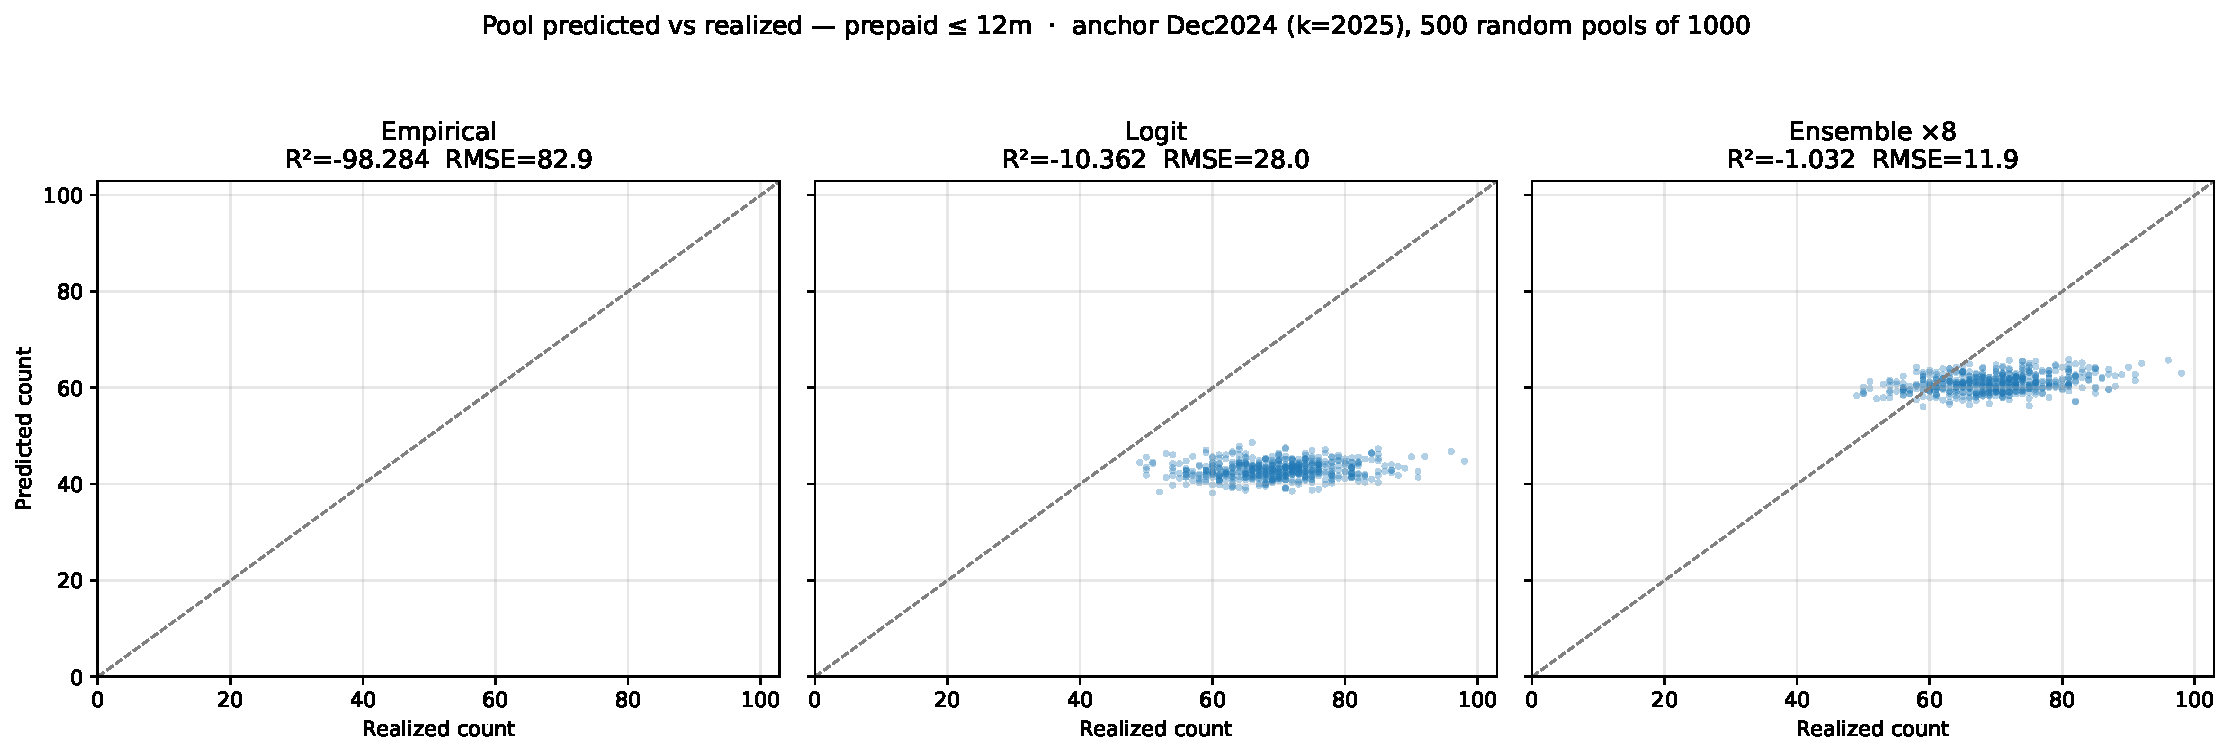
\includegraphics[width=0.95\textwidth]{figs/F4.1_scatter_random_prepaid.pdf}
\caption[Predicted versus realised pool prepayment counts, random
pools]{Predicted versus realised twelve-month prepayment counts, 500
random pools of 1{,}000 loans at the Dec2024 anchor, by model.  The
dashed line is $45^\circ$.  Level calibration improves
empirical\,$\to$\,logit\,$\to$\,ensemble (RMSE $82.9/28.0/11.9$);
$R^2$ is uninformative for homogeneous random pools (see
text).}\label{fig:poolscatter}
\end{figure}

\begin{table}[htbp]\centering\small
\caption[Characteristic-bucket pool accuracy by model, outcome, and
anchor]{Pool-level $R^2$ and RMSE on the characteristic buckets
(credit$\,\times\,$rate$\,\times\,$LTV cells, $\geq2{,}000$ loans each)
by model, outcome, and anchor.  The interpretable cross-pool panel;
random-pool $R^2$ is discussed in the text.  RMSE is in loans.  Shock-type
dependence: covariate models dominate off-COVID and under the rate
shock, but the empirical floor is most robust at the 2020 forbearance
break.}\label{tab:poolaccuracy}
% Source: outputs/tables/pool_level/t_m14_pool_counts.json (M14, full run).
% Characteristic-bucket panel (FICO x orig-rate-quartile x LTV, >=2000 loans/cell): the
% interpretable cross-pool metric. Random-pool R^2 is uninformative by construction
% (homogeneous ~1000-loan draws) and is discussed in text, not tabulated. For the rare
% 60+ DPD outcome read RMSE, not R^2 (>=~16 buckets makes R^2 unstable). Caption in chapter4.tex.
\begin{tabular}{llrrrrrr}
\toprule
 & & \multicolumn{3}{c}{$R^2$} & \multicolumn{3}{c}{RMSE (loans)} \\
\cmidrule(lr){3-5}\cmidrule(lr){6-8}
Outcome & Anchor & Emp. & Logit & Ens. & Emp. & Logit & Ens. \\
\midrule
\multirow{5}{*}{Prepaid} & Dec2014 & 0.575 & 0.980 & 0.981 & 1517 & 328 & 320 \\
 & Dec2018 & 0.744 & 0.607 & 0.791 & 1118 & 1387 & 1011 \\
 & Dec2019 & 0.647 & 0.537 & 0.449 & 3054 & 3500 & 3817 \\
 & Dec2022 & -4.616 & 0.742 & 0.848 & 3303 & 708 & 542 \\
 & Dec2024 & -1.455 & 0.651 & 0.939 & 2627 & 991 & 415 \\
\midrule
\multirow{5}{*}{60+ DPD} & Dec2014 & -4.525 & -0.782 & 0.299 & 449 & 255 & 160 \\
 & Dec2018 & -8.699 & -1.230 & -0.390 & 423 & 203 & 160 \\
 & Dec2019 & -0.165 & -0.467 & -0.464 & 591 & 663 & 663 \\
 & Dec2022 & -17.181 & -0.155 & 0.635 & 514 & 129 & 73 \\
 & Dec2024 & -16.461 & -0.063 & 0.261 & 471 & 116 & 97 \\
\bottomrule
\end{tabular}

\end{table}

\subsection{Economic translation: speed, timing, and price errors}

Restating these count comparisons in valuation units
(Section~\ref{subsec:meth-econ}) sharpens the contribution.
Table~\ref{tab:econerrors} reports mean absolute speed (CPR), timing
(weighted-average life), and price errors on the characteristic
buckets, with the ensemble-versus-logit reduction in the last column;
all errors are model-implied minus realised-speed valuation through the
same engine, so the price column isolates the prepayment forecast.  The
headline is the price row, \textbf{reported per anchor because it
inverts at COVID and a pooled average would conceal that}: the ensemble
cuts the logit's mean absolute price error by $+18\%$ at Dec2014
($0.148\to0.121$ per 100 face), $+25\%$ at Dec2018
($0.560\to0.418$), $+31\%$ at Dec2022 ($0.254\to0.176$), and $+48\%$ at
Dec2024 ($0.233\to0.122$), but by $-1\%$ at the Dec2019 COVID anchor
($0.583\to0.587$) --- the same inversion as the counts, now in price.
The absolute magnitudes are economically modest in aggregate (fractions
of a point per 100 of face), as expected when the discount curve is
fixed and the pools diversify idiosyncratic timing; the action is in
\emph{where} the error concentrates.

Figure~\ref{fig:pricerrorbuckets} maps the signed price error across
credit\,$\times$\,rate cells at the Dec2022 rate-spike anchor, per
model.  The empirical matrix misprices everywhere ($-0.7$ to $-1.2$ per
100, over-predicting prepayment uniformly).  The logit's error is
benign in the low-rate cells but \textbf{concentrates in the
high-incentive top rate quartile} --- $-0.35$ to $-0.61$ per 100, where
its linear-in-incentive form over-fires prepayment on high-coupon loans
whose incentive had in fact collapsed after the 2022 rate rise.  The
ensemble compresses exactly those cells to $-0.15$ to $-0.32$.  This is
the pricing mirror of the prepayment S-curve of
Section~\ref{subsec:data-eda-single}: the linear model breaks where the
hazard is most curved, and that is where dollars of mispricing collect.

\begin{table}[htbp]\centering\small
\caption[Pool CPR, weighted-average-life, and price errors by model and
anchor]{Mean absolute CPR (percentage points), weighted-average-life
(months), and price (per 100 face) error on the characteristic buckets,
by model and anchor, with the ensemble-versus-logit reduction.  Errors
are model-implied minus realised-speed valuation through the same
level-pay engine and discount curve.  The price row is the headline;
reported per anchor because the 2020 anchor
inverts.}\label{tab:econerrors}
% Source: outputs/tables/pool_level/t_m15_econ_errors.json (M15b).
% Characteristic-bucket panel. Each model cell is the mean |error| over the bucket pools;
% errors = model-implied minus realized-SMM valuation through the same level-pay engine
% (identical WAC/WAM/UPB, WAC-25bp curve, so price dispersion isolates the prepay model).
% Last column = ensemble-vs-logit reduction in that row's mean |error| (the price row is the
% headline). Reported per anchor, never pooled (the Dec2019 COVID anchor inverts). Caption in chapter4.tex.
\begin{tabular}{llrrrr}
\toprule
Metric & Anchor & Empirical & Logit & Ensemble & Ens.\,vs\,Logit \\
\midrule
\multirow{5}{*}{\shortstack[l]{Price error\\(per 100 face)}} & Dec2014 & 0.228 & 0.148 & 0.121 & $+18\%$ \\
 & Dec2018 & 0.205 & 0.560 & 0.418 & $+25\%$ \\
 & Dec2019 & 0.552 & 0.583 & 0.587 & $-1\%$ \\
 & Dec2022 & 1.068 & 0.254 & 0.176 & $+31\%$ \\
 & Dec2024 & 0.657 & 0.233 & 0.122 & $+48\%$ \\
\midrule
\multirow{5}{*}{\shortstack[l]{CPR error\\(pp)}} & Dec2014 & 4.30 & 2.34 & 3.28 & $-40\%$ \\
 & Dec2018 & 3.14 & 6.28 & 4.79 & $+24\%$ \\
 & Dec2019 & 17.08 & 16.69 & 17.41 & $-4\%$ \\
 & Dec2022 & 11.80 & 2.69 & 1.56 & $+42\%$ \\
 & Dec2024 & 9.30 & 2.02 & 0.50 & $+75\%$ \\
\midrule
\multirow{5}{*}{\shortstack[l]{WAL error\\(months)}} & Dec2014 & 14.8 & 10.1 & 8.1 & $+20\%$ \\
 & Dec2018 & 13.3 & 38.5 & 28.5 & $+26\%$ \\
 & Dec2019 & 34.0 & 35.7 & 35.8 & $0\%$ \\
 & Dec2022 & 72.0 & 18.9 & 12.9 & $+32\%$ \\
 & Dec2024 & 42.6 & 16.2 & 9.3 & $+43\%$ \\
\bottomrule
\end{tabular}

\end{table}

\begin{figure}[htbp]\centering
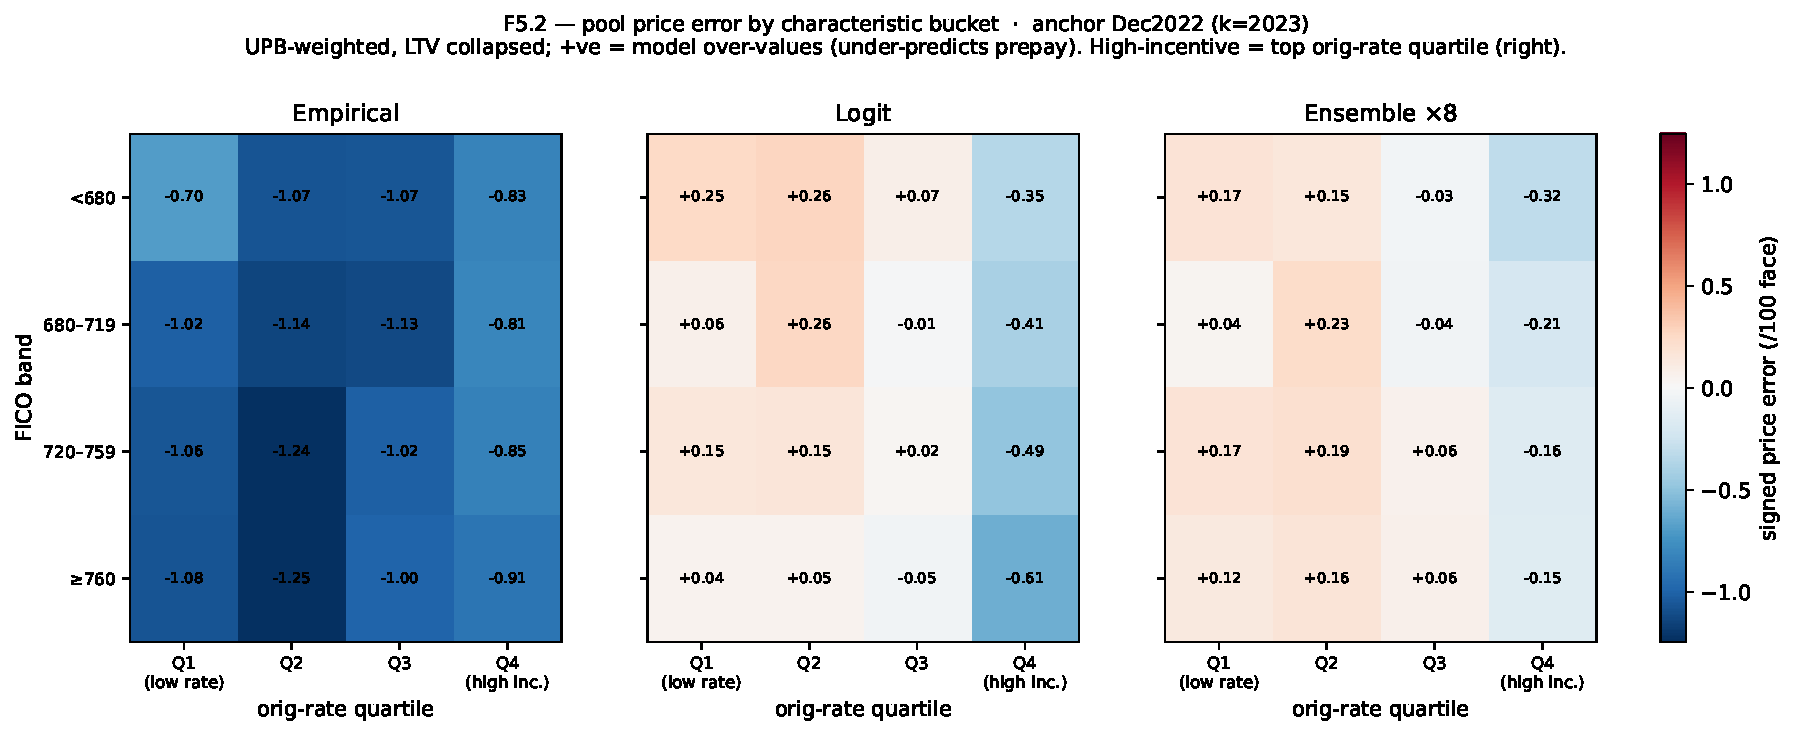
\includegraphics[width=0.95\textwidth]{figs/F5.2_price_error_buckets.pdf}
\caption[Pool price error by characteristic bucket and model]{Signed
price error (per 100 face, UPB-weighted, LTV collapsed) by
credit\,$\times$\,original-rate-quartile cell at the Dec2022 anchor, per
model; positive means the model over-values the pool by under-predicting
prepayment.  The logit's error concentrates in the high-incentive top
rate quartile (right column), which the ensemble
compresses.}\label{fig:pricerrorbuckets}
\end{figure}

\paragraph{Why price is not simply average CPR.}  A pool's price
depends on the \emph{timing} of returned principal --- the full monthly
speed path and hence the weighted-average life --- not on the average
speed alone, which is what makes the cashflow engine more than a
relabelling of CPR.  The two can even rank models differently: at
Dec2014 the logit's mean CPR error is the smaller ($2.34$ against the
ensemble's $3.28$ percentage points), yet the ensemble still prices the
buckets better ($+18\%$ lower price error), because it places its
prepayments at more accurate \emph{months}.  Reassuringly, the engine
is internally coherent --- across all pools and anchors the sign of the
price error agrees with the sign of the weighted-average-life error in
$99.4$--$100\%$ of cases (slower prepayment $\Rightarrow$ longer life
$\Rightarrow$ higher price on these premium pass-throughs).  The
price-versus-CPR sign disagreements occur \emph{only} where the CPR
error is itself negligible (median $0.5$--$1.6$ against $2$--$4.5$
percentage points where they agree): when average speeds nearly match,
timing is what remains, and only the price and life errors can see it.

\paragraph{The frozen-anchor caveat.}  These are
\emph{prepayment-model} valuation errors at a fixed discount curve with
the macroeconomic environment frozen at each anchor, not full
option-adjusted spreads (Section~\ref{subsec:meth-econ}).  The
single regime where this assumption bites hardest is the one it is
designed to expose: at Dec2019 every model under-predicts the realised
$33\%$ CPR by about seventeen percentage points, because all are blind
to the March-2020 rate collapse and refinancing wave that no $t_0$
covariate could anticipate.  Far from a flaw, this is the cleanest
statement of the design's boundary --- it prices the prepayment model,
holding the world fixed --- and it is exactly why the value of
nonlinearity must be read as regime-conditional rather than as a single
headline number.
          % Loan-level results (tuning window + rolling backtest)
% ============================================================
%  Chapter 5 — Pool-level valuation
%  Moved verbatim (June 2026 skeleton pass) from chapter4.tex §4.3:
%  the "from loans to pools" roll-forward results + economic
%  translation (Phase 3, M13–M15). The two former subsections are
%  promoted to sections §5.1/§5.2; the §4.3 lead paragraph now opens
%  the chapter. The four Phase-3 artifacts are F4.1 (fig:poolscatter),
%  T4.2 (tab:poolaccuracy), T5.1 (tab:econerrors), and F5.2
%  (fig:pricerrorbuckets); .tex tables regenerate via
%  dev/model/make_pool_tex.py from the committed M14/M15b JSON. All
%  numbers/tables/figures trace to outputs/{tables,figures}/pool_level.
% ============================================================

\chapter{Pool-level valuation}
\label{chap:poollevel}

The loan-level models of Section~\ref{sec:results-rolling} are now
aggregated to pools by the roll-forward of
Section~\ref{subsec:meth-pools}: for every loan alive at a window
anchor $t_0{=}\text{Dec}(k{-}1)$, the window-$k$ model's monthly
transition matrices are composed twelve steps forward to a horizon
event probability, and pool counts and speed paths follow from
\eqref{eq:poolcount} and Section~\ref{subsec:meth-econ}.  Only the
deterministic covariates evolve along the chain (loan age, remaining
term, calendar seasonality); the entire macroeconomic block --- rate
incentive, unemployment, house-price growth --- is \emph{frozen at the
anchor}, so every prediction is conditional on the $t_0$ environment.
Five regime-spanning anchors are scored, each with its own frozen
window-$k$ models: Dec2014 (calm), Dec2018 (late cycle), Dec2019
(entering the COVID forbearance shock), Dec2022 (the rate spike), and
Dec2024.

\section{Pool-level accuracy and the regime exhibit}

Figure~\ref{fig:poolscatter} is the flagship pool exhibit:
predicted versus realised twelve-month prepayment counts for the 500
random pools at Dec2024, one panel per model.  The improvement in
\emph{level} is stark --- the covariate-free empirical matrix predicts
roughly $2.5\times$ too many prepayments (its flat CPR floor ignores
that the 2024 cohort is deeply out of the money), the logit closes most
of the gap, and the ensemble cloud sits nearest the diagonal (RMSE
$82.9 \to 28.0 \to 11.9$ loans).  The $R^2$ values are all negative
even for the ensemble: random pools are near-homogeneous $1{,}000$-loan
draws, so cross-pool realised variance is tiny and $R^2$ is dominated
by a small level bias --- the random scheme tests \emph{level}
calibration, not cross-pool discrimination, which is why the
discriminating metric is read from the characteristic buckets instead.

Table~\ref{tab:poolaccuracy} gives that characteristic-bucket panel ---
$R^2$ and RMSE by model, outcome, and anchor --- and it is the regime
exhibit promised in Section~\ref{sec:intro-contributions}: a time
series of the value of nonlinearity, not a single verdict.
\textbf{Which model prices a pool best depends on whether the shock
lands in a covariate-captured channel.}  In calm and late-cycle
regimes the covariate models dominate (Dec2014 prepaid $R^2$
$0.58/0.98/0.98$ for empirical/logit/ensemble).  Under the
\emph{rate/prepayment-incentive shock} of 2022--24 --- precisely the
channel the rate-incentive covariates encode --- the empirical matrix
collapses to large negative $R^2$ ($-4.62$ at Dec2022, $-1.46$ at
Dec2024) while the ensemble is strongest ($0.85$, $0.94$; RMSE $415$
against the logit's $991$ at Dec2024).  But under the 2020
\emph{forbearance/credit shock} the ordering \emph{inverts}: at Dec2019
the assumption-free empirical floor is best ($R^2\,0.65$) and the
ensemble is worst ($0.45$), because the ensemble bakes in hardest a
pre-COVID prepayment signal that March 2020 abruptly invalidates.  For
the rare serious-delinquency outcome RMSE is the reliable metric (with
$\sim$16 buckets $R^2$ is unstable across all models), and the ensemble
is the only model with positive $60{+}$\,DPD $R^2$ at the 2022 and 2024
anchors.

\begin{figure}[htbp]\centering
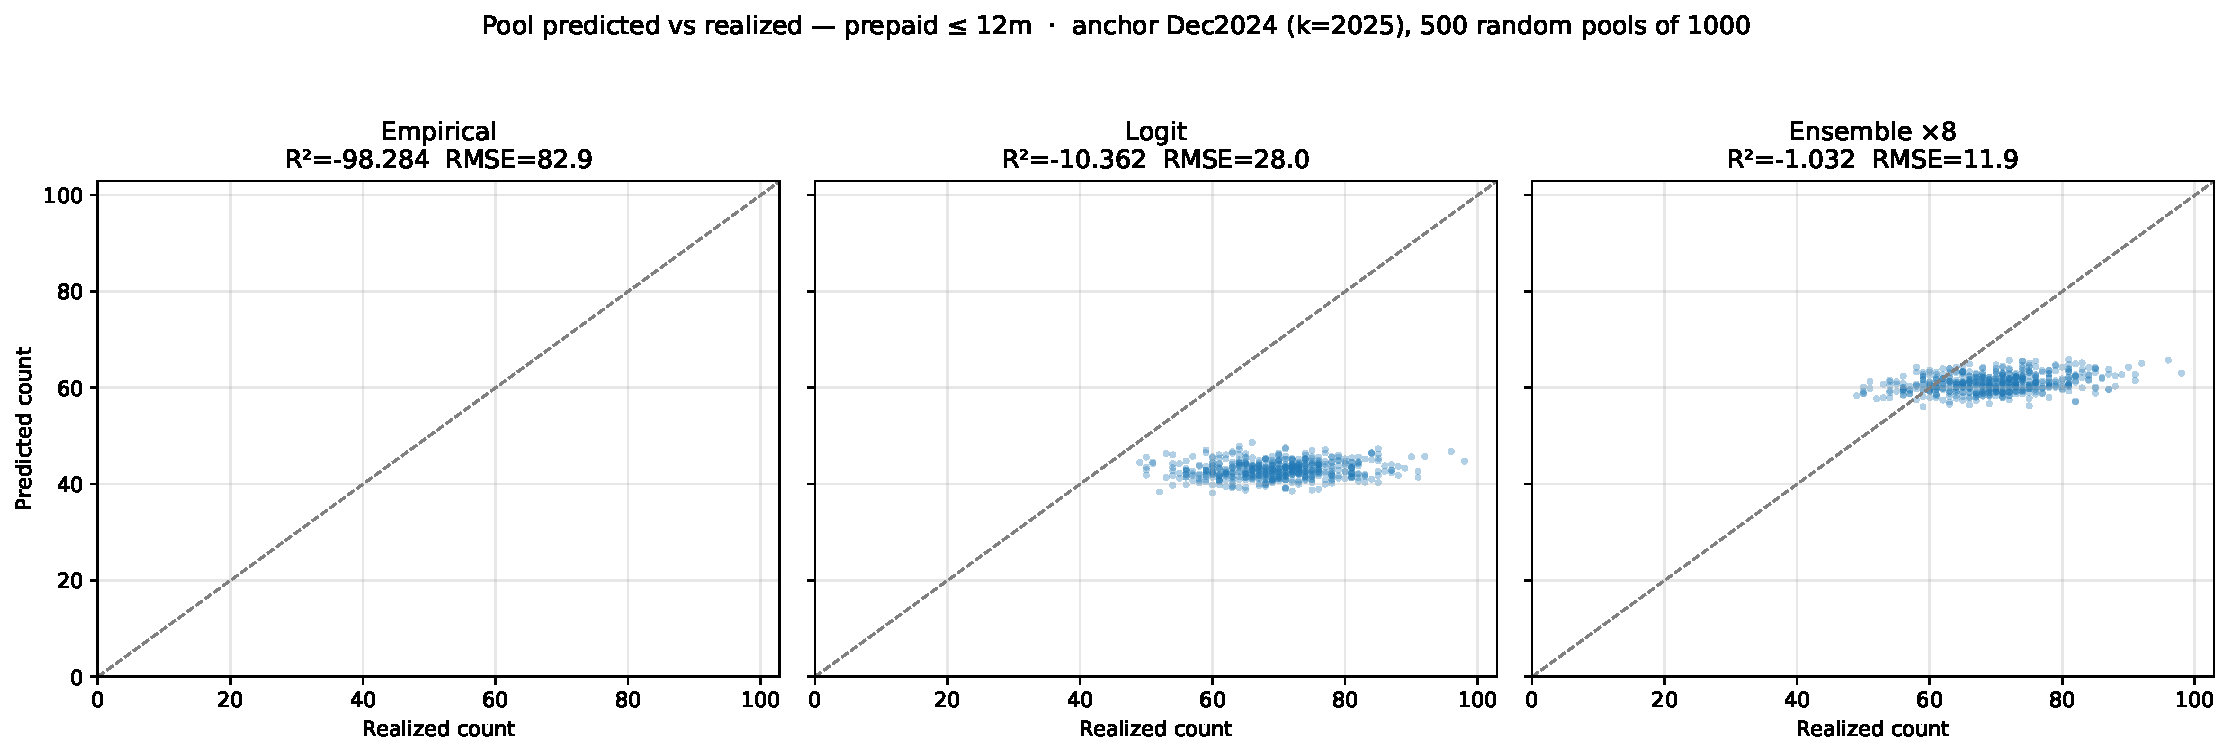
\includegraphics[width=0.95\textwidth]{figs/F4.1_scatter_random_prepaid.pdf}
\caption[Predicted versus realised pool prepayment counts, random
pools]{Predicted versus realised twelve-month prepayment counts, 500
random pools of 1{,}000 loans at the Dec2024 anchor, by model.  The
dashed line is $45^\circ$.  Level calibration improves
empirical\,$\to$\,logit\,$\to$\,ensemble (RMSE $82.9/28.0/11.9$);
$R^2$ is uninformative for homogeneous random pools (see
text).}\label{fig:poolscatter}
\end{figure}

\begin{table}[htbp]\centering\small
\caption[Characteristic-bucket pool accuracy by model, outcome, and
anchor]{Pool-level $R^2$ and RMSE on the characteristic buckets
(credit$\,\times\,$rate$\,\times\,$LTV cells, $\geq2{,}000$ loans each)
by model, outcome, and anchor.  The interpretable cross-pool panel;
random-pool $R^2$ is discussed in the text.  RMSE is in loans.  Shock-type
dependence: covariate models dominate off-COVID and under the rate
shock, but the empirical floor is most robust at the 2020 forbearance
break.}\label{tab:poolaccuracy}
% Source: outputs/tables/pool_level/t_m14_pool_counts.json (M14, full run).
% Characteristic-bucket panel (FICO x orig-rate-quartile x LTV, >=2000 loans/cell): the
% interpretable cross-pool metric. Random-pool R^2 is uninformative by construction
% (homogeneous ~1000-loan draws) and is discussed in text, not tabulated. For the rare
% 60+ DPD outcome read RMSE, not R^2 (>=~16 buckets makes R^2 unstable). Caption in chapter4.tex.
\begin{tabular}{llrrrrrr}
\toprule
 & & \multicolumn{3}{c}{$R^2$} & \multicolumn{3}{c}{RMSE (loans)} \\
\cmidrule(lr){3-5}\cmidrule(lr){6-8}
Outcome & Anchor & Emp. & Logit & Ens. & Emp. & Logit & Ens. \\
\midrule
\multirow{5}{*}{Prepaid} & Dec2014 & 0.575 & 0.980 & 0.981 & 1517 & 328 & 320 \\
 & Dec2018 & 0.744 & 0.607 & 0.791 & 1118 & 1387 & 1011 \\
 & Dec2019 & 0.647 & 0.537 & 0.449 & 3054 & 3500 & 3817 \\
 & Dec2022 & -4.616 & 0.742 & 0.848 & 3303 & 708 & 542 \\
 & Dec2024 & -1.455 & 0.651 & 0.939 & 2627 & 991 & 415 \\
\midrule
\multirow{5}{*}{60+ DPD} & Dec2014 & -4.525 & -0.782 & 0.299 & 449 & 255 & 160 \\
 & Dec2018 & -8.699 & -1.230 & -0.390 & 423 & 203 & 160 \\
 & Dec2019 & -0.165 & -0.467 & -0.464 & 591 & 663 & 663 \\
 & Dec2022 & -17.181 & -0.155 & 0.635 & 514 & 129 & 73 \\
 & Dec2024 & -16.461 & -0.063 & 0.261 & 471 & 116 & 97 \\
\bottomrule
\end{tabular}

\end{table}

\section{Economic translation: speed, timing, and price errors}

Restating these count comparisons in valuation units
(Section~\ref{subsec:meth-econ}) sharpens the contribution.
Table~\ref{tab:econerrors} reports mean absolute speed (CPR), timing
(weighted-average life), and price errors on the characteristic
buckets, with the ensemble-versus-logit reduction in the last column;
all errors are model-implied minus realised-speed valuation through the
same engine, so the price column isolates the prepayment forecast.  The
headline is the price row, \textbf{reported per anchor because it
inverts at COVID and a pooled average would conceal that}: the ensemble
cuts the logit's mean absolute price error by $+18\%$ at Dec2014
($0.148\to0.121$ per 100 face), $+25\%$ at Dec2018
($0.560\to0.418$), $+31\%$ at Dec2022 ($0.254\to0.176$), and $+48\%$ at
Dec2024 ($0.233\to0.122$), but by $-1\%$ at the Dec2019 COVID anchor
($0.583\to0.587$) --- the same inversion as the counts, now in price.
The absolute magnitudes are economically modest in aggregate (fractions
of a point per 100 of face), as expected when the discount curve is
fixed and the pools diversify idiosyncratic timing; the action is in
\emph{where} the error concentrates.

Figure~\ref{fig:pricerrorbuckets} maps the signed price error across
credit\,$\times$\,rate cells at the Dec2022 rate-spike anchor, per
model.  The empirical matrix misprices everywhere ($-0.7$ to $-1.2$ per
100, over-predicting prepayment uniformly).  The logit's error is
benign in the low-rate cells but \textbf{concentrates in the
high-incentive top rate quartile} --- $-0.35$ to $-0.61$ per 100, where
its linear-in-incentive form over-fires prepayment on high-coupon loans
whose incentive had in fact collapsed after the 2022 rate rise.  The
ensemble compresses exactly those cells to $-0.15$ to $-0.32$.  This is
the pricing mirror of the prepayment S-curve of
Section~\ref{subsec:data-eda-single}: the linear model breaks where the
hazard is most curved, and that is where dollars of mispricing collect.

\begin{table}[htbp]\centering\small
\caption[Pool CPR, weighted-average-life, and price errors by model and
anchor]{Mean absolute CPR (percentage points), weighted-average-life
(months), and price (per 100 face) error on the characteristic buckets,
by model and anchor, with the ensemble-versus-logit reduction.  Errors
are model-implied minus realised-speed valuation through the same
level-pay engine and discount curve.  The price row is the headline;
reported per anchor because the 2020 anchor
inverts.}\label{tab:econerrors}
% Source: outputs/tables/pool_level/t_m15_econ_errors.json (M15b).
% Characteristic-bucket panel. Each model cell is the mean |error| over the bucket pools;
% errors = model-implied minus realized-SMM valuation through the same level-pay engine
% (identical WAC/WAM/UPB, WAC-25bp curve, so price dispersion isolates the prepay model).
% Last column = ensemble-vs-logit reduction in that row's mean |error| (the price row is the
% headline). Reported per anchor, never pooled (the Dec2019 COVID anchor inverts). Caption in chapter4.tex.
\begin{tabular}{llrrrr}
\toprule
Metric & Anchor & Empirical & Logit & Ensemble & Ens.\,vs\,Logit \\
\midrule
\multirow{5}{*}{\shortstack[l]{Price error\\(per 100 face)}} & Dec2014 & 0.228 & 0.148 & 0.121 & $+18\%$ \\
 & Dec2018 & 0.205 & 0.560 & 0.418 & $+25\%$ \\
 & Dec2019 & 0.552 & 0.583 & 0.587 & $-1\%$ \\
 & Dec2022 & 1.068 & 0.254 & 0.176 & $+31\%$ \\
 & Dec2024 & 0.657 & 0.233 & 0.122 & $+48\%$ \\
\midrule
\multirow{5}{*}{\shortstack[l]{CPR error\\(pp)}} & Dec2014 & 4.30 & 2.34 & 3.28 & $-40\%$ \\
 & Dec2018 & 3.14 & 6.28 & 4.79 & $+24\%$ \\
 & Dec2019 & 17.08 & 16.69 & 17.41 & $-4\%$ \\
 & Dec2022 & 11.80 & 2.69 & 1.56 & $+42\%$ \\
 & Dec2024 & 9.30 & 2.02 & 0.50 & $+75\%$ \\
\midrule
\multirow{5}{*}{\shortstack[l]{WAL error\\(months)}} & Dec2014 & 14.8 & 10.1 & 8.1 & $+20\%$ \\
 & Dec2018 & 13.3 & 38.5 & 28.5 & $+26\%$ \\
 & Dec2019 & 34.0 & 35.7 & 35.8 & $0\%$ \\
 & Dec2022 & 72.0 & 18.9 & 12.9 & $+32\%$ \\
 & Dec2024 & 42.6 & 16.2 & 9.3 & $+43\%$ \\
\bottomrule
\end{tabular}

\end{table}

\begin{figure}[htbp]\centering
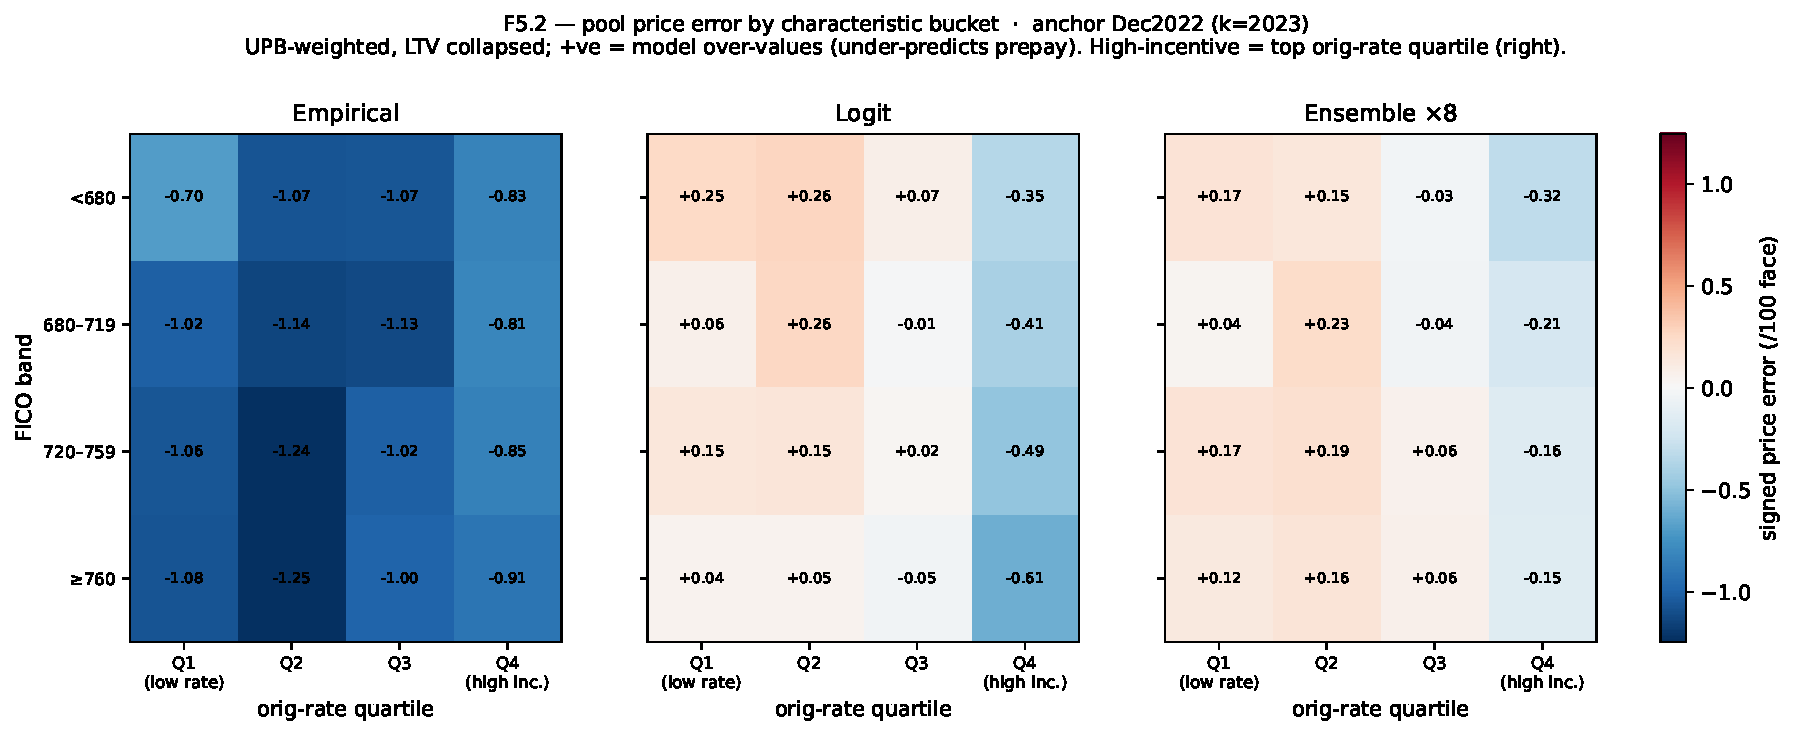
\includegraphics[width=0.95\textwidth]{figs/F5.2_price_error_buckets.pdf}
\caption[Pool price error by characteristic bucket and model]{Signed
price error (per 100 face, UPB-weighted, LTV collapsed) by
credit\,$\times$\,original-rate-quartile cell at the Dec2022 anchor, per
model; positive means the model over-values the pool by under-predicting
prepayment.  The logit's error concentrates in the high-incentive top
rate quartile (right column), which the ensemble
compresses.}\label{fig:pricerrorbuckets}
\end{figure}

\paragraph{Why price is not simply average CPR.}  A pool's price
depends on the \emph{timing} of returned principal --- the full monthly
speed path and hence the weighted-average life --- not on the average
speed alone, which is what makes the cashflow engine more than a
relabelling of CPR.  The two can even rank models differently: at
Dec2014 the logit's mean CPR error is the smaller ($2.34$ against the
ensemble's $3.28$ percentage points), yet the ensemble still prices the
buckets better ($+18\%$ lower price error), because it places its
prepayments at more accurate \emph{months}.  Reassuringly, the engine
is internally coherent --- across all pools and anchors the sign of the
price error agrees with the sign of the weighted-average-life error in
$99.4$--$100\%$ of cases (slower prepayment $\Rightarrow$ longer life
$\Rightarrow$ higher price on these premium pass-throughs).  The
price-versus-CPR sign disagreements occur \emph{only} where the CPR
error is itself negligible (median $0.5$--$1.6$ against $2$--$4.5$
percentage points where they agree): when average speeds nearly match,
timing is what remains, and only the price and life errors can see it.

\paragraph{The frozen-anchor caveat.}  These are
\emph{prepayment-model} valuation errors at a fixed discount curve with
the macroeconomic environment frozen at each anchor, not full
option-adjusted spreads (Section~\ref{subsec:meth-econ}).  The
single regime where this assumption bites hardest is the one it is
designed to expose: at Dec2019 every model under-predicts the realised
$33\%$ CPR by about seventeen percentage points, because all are blind
to the March-2020 rate collapse and refinancing wave that no $t_0$
covariate could anticipate.  Far from a flaw, this is the cleanest
statement of the design's boundary --- it prices the prepayment model,
holding the world fixed --- and it is exactly why the value of
nonlinearity must be read as regime-conditional rather than as a single
headline number.
          % Pool-level valuation (roll-forward + economic translation)
\chapter{Conclusions}
\label{chap:conclusions}

% TODO after Phase 3: headline NLL/AUC results, regime stability, pool-level
% economic translation, limitations (frozen macro, state-level granularity,
% final-revision series), future work (portfolio sorts, macro scenarios).


%appendices
\appendix
\chapter{Supplementary tables and figures}
\label{app:supplementary}

% TODO: width-sweep table (M12), full Table A grid, per-window diagnostics.

\chapter{Reproducibility}
\label{app:reproducibility}

% TODO: pipeline summary, run-folder/manifest conventions, hardware/software
% (GPU models per session, torch 2.8.0), data snapshot dates.

% ============================================================
%  Appendix C — Deep-Learning Foundations
%
%  DRAFT (AI-assisted, June 2026). This appendix grounds the
%  deep-learning machinery applied in Chapter 2 in the theory and
%  reading list of the MSc Deep Learning course. It is written as
%  scaffolding: revise into your own voice, trim anything the examiner
%  would consider textbook padding, and keep only what earns its place.
%  Every claim is cited; cross-references point back to the methods in
%  Chapter 2 so the appendix documents *why* each choice is principled
%  rather than restating it.
% ============================================================

\chapter{Deep-Learning Foundations}
\label{app:dlfoundations}
% SUGGESTED TRIM: KEEP but tighten. Opening framing is fine; trim sentences that only announce "this appendix is background" rather than doing work.

The methodology of Chapter~\ref{chap:methodology} applies a sequence of
deep-learning tools --- a multilayer network trained by stochastic
gradient descent, adaptive optimisation, dropout, $\ell_2$
regularisation, early stopping, and ensembling --- as established
technique, without pausing to justify them. This appendix supplies
that justification, drawing on the standard references
\citep{goodfellow2016,hastie2009}. It is deliberately background; the
intent is to record the theoretical results that make each modelling
choice in Chapter~\ref{chap:methodology} principled rather than
heuristic, and to place the study in the lineage of machine learning
applied to credit and asset-pricing problems.

\section{Function classes and universal approximation}
\label{sec:dlf-approx}
% SUGGESTED TRIM: KEEP (defends a Ch.2 choice). Justifies the deep hypothesis class over the logit; compress the textbook universal-approximation exposition, retain the "logit = zero-hidden-layer boundary case" point.

The estimand \eqref{eq:object} is a conditional distribution over next
month's state, and the modelling question is how flexibly a candidate
$p_\theta(\cdot\mid x)$ is allowed to depend on the covariates $x$. The
multinomial logit \eqref{eq:logit} confines that dependence to a
log-linear form; the deep network \eqref{eq:mlp} does not. The
theoretical warrant for the latter is the universal approximation
theorem: a feedforward network with a single hidden layer of
sufficiently many units and a non-polynomial activation can approximate
any continuous function on a compact set to arbitrary accuracy
\citep{cybenko1989,hornik1991}. The result certifies that the
hypothesis class of \eqref{eq:mlp} contains, in the limit of width, the
true transition surface whose nonlinearity \citet{sirignano2021} claim
is economically material --- so a deep model's empirical edge over the
logit reflects a representable feature of the data, not an artefact.
The theorem is, however, existential and says nothing about whether a
finite network can be \emph{found} by training, nor how much data the
search needs; depth (searched over $L\in\{1,3,5,7\}$ in
Section~\ref{subsec:meth-nn}) is the practically more economical route
to the same expressive power, building the interaction hierarchy ---
incentive$\times$credit-score and the like --- through composition
rather than width. The logit is then exactly the zero-hidden-layer
boundary case of the same class (Section~\ref{subsec:meth-logit}),
which is what makes the model hierarchy a controlled comparison.

\section{Training: backpropagation and stochastic gradient descent}
\label{sec:dlf-sgd}
% SUGGESTED TRIM: KEEP core (defends the two-level shuffle + Horvitz-Thompson weights = unbiased minibatch gradient). Compress the backprop / Robbins-Monro / Bottou history.

Fitting \eqref{eq:mlp} means minimising the weighted negative
log-likelihood \eqref{eq:weightednll} over the parameters $\theta$.
The gradient $\nabla_\theta\widehat{\mathcal L}$ is computed by
backpropagation --- reverse-mode automatic differentiation, the
reverse accumulation of the chain rule through the network's
computational graph \citep{rumelhart1986} --- which yields all partial
derivatives at the cost of a constant multiple of one forward
evaluation, and is what PyTorch's autograd implements. Because the
objective is an average over $\sim$$10^{9}$ loan-months, full-batch
gradients are infeasible, and the parameters are updated on minibatch
estimates: stochastic gradient descent, whose convergence under
decreasing step sizes traces to the stochastic-approximation theory of
\citet{robbins1951} and is treated for the modern large-scale setting
by \citet{bottou2018}. SGD's guarantees rest on minibatch gradients
being \emph{unbiased} estimates of the full-data gradient. Two design
choices in Chapter~\ref{chap:methodology} exist precisely to protect
that property: the loan-keyed two-level shuffle of
Section~\ref{sec:meth-shards}, which keeps each minibatch an
approximately uniform cross-section despite vintage-grouped storage,
and the Horvitz--Thompson inverse-probability weights in
\eqref{eq:weightednll}, which keep the thinned-sample loss --- and
hence its gradient --- an unbiased estimate of the full-sample loss.

\section{Adaptive optimisers}
\label{sec:dlf-adam}
% SUGGESTED TRIM: KEEP (defends a Ch.2 choice: Adam used identically for the logit control, so the comparison varies architecture alone). Already short.

Plain SGD with a single global step size is sensitive to feature
scaling and curvature anisotropy, both severe here given embeddings and
heavy-tailed balances. The training runs therefore use Adam
\citep{kingma2015}, which maintains per-parameter exponential moving
averages of the gradient and its square and rescales each update by the
latter, combining the per-coordinate adaptivity of RMSprop
\citep{tieleman2012} with momentum. This is the optimiser referenced in
the loan-level model plan (Adam, learning rate $\sim$$10^{-3}$ with
decay-on-plateau), and it is used identically for the logit control of
Section~\ref{subsec:meth-logit}, so that the network-versus-logit
comparison varies architecture alone and not the optimisation
procedure.

\section{Regularisation, ensembling, and normalisation}
\label{sec:dlf-reg}
% SUGGESTED TRIM: MIXED. KEEP the batch/layer-norm OMISSION defence (justifies a Ch.2 design choice); COMPRESS the textbook ridge / dropout / bagging recap.

A width-200, several-layer network has ample capacity to overfit rare
credit events, and Section~\ref{subsec:meth-nn} deploys four classical
controls. The $\ell_2$ penalty (weight decay) is ridge regularisation
in the sense of \citet{hastie2009}, shrinking parameters toward zero and
trading a little bias for reduced variance. Dropout
\citep{dropout} randomly zeroes hidden units during training, which
acts as an implicit ensemble over subnetworks and a stochastic
regulariser. Early stopping on the window's validation likelihood halts
the fit before it specialises to training noise --- a form of
regularisation through optimisation budget. The headline ensemble, an
average of $K{=}8$ independently initialised networks, is bagging-style
variance reduction \citep{hastie2009}: averaging quasi-independent
predictors lowers the variance component of generalisation error, which
for high-capacity models fit by a stochastic procedure is substantial.

Normalisation layers --- batch normalisation \citep{ioffe2015} and layer
normalisation \citep{ba2016} --- are part of the standard deep-learning
toolkit and are covered in the course, but the loan-level model does
\emph{not} use them. For this tabular network the per-window
standardisation of continuous covariates described in
Section~\ref{sec:meth-features} supplies the input conditioning that
batch normalisation would otherwise provide, and avoiding
batch-statistic layers keeps the strictly out-of-sample design of
Section~\ref{sec:meth-design} clean (no train-time batch statistics
leaking across the temporal split). This is a deliberate omission, not
an oversight, and is noted here for completeness.

\section{Architectures beyond the feedforward network}
\label{sec:dlf-arch}
% SUGGESTED TRIM: KEEP the "why a plain feedforward net" argument (defends the Ch.2 Markov framing); COMPRESS the ResNet/LSTM/Transformer/GAN survey to a sentence.

The course surveys architectures this study does not use ---
residual networks \citep{he2016}, recurrent networks such as the LSTM
\citep{hochreiter1997}, attention-based transformers
\citep{vaswani2017}, and generative adversarial networks
\citep{goodfellow2014gan} --- and it is worth stating why a plain
feedforward network is the right tool here. The modelling object
\eqref{eq:object} is a \emph{one-month} conditional transition given
the current state and covariates; the Markov framing of
Section~\ref{sec:meth-model} already encodes the loan's dynamics
through the state feature and loan age, so the temporal dependence that
would motivate a recurrent or attention model is handled by the
state-space construction rather than by the network. Residual
connections and normalisation address optimisation pathologies of very
deep networks that do not arise at depths $L\le 7$. The feedforward
choice is thus a consequence of the problem's structure, made against
the full menu of alternatives rather than by default.

\section{Machine learning in credit and asset pricing}
\label{sec:dlf-lineage}
% SUGGESTED TRIM: KEEP (literature positioning, not padding). The Gu-Kelly-Xiu "levels not ranks" link to the pool-level pricing exercise earns its place.

The study sits in an established line of work applying flexible
machine learning to financial prediction. \citet{sirignano2021} ---
the paper this dissertation tests on a cleaner dataset --- is the
direct antecedent for deep learning of mortgage transition risk.
Earlier, \citet{khandani2010} showed machine-learning models improve
consumer credit-risk forecasts, and \citet{fuster2022} examine the
distributional consequences of machine learning in credit markets,
both relevant to the credit-event side of the transition model.
\citet{gukellyxiu2020} establish the value of nonlinear machine
learning for the levels of expected returns in empirical asset
pricing --- the methodological cousin of the pool-level pricing
exercise in Section~\ref{sec:meth-pool}, where prediction levels (not
merely rankings) are what the valuation consumes. Reinforcement
learning, surveyed for finance by \citet{bai2025} and developed in
\citet{suttonbarto2018}, lies outside this study's supervised framing
but is the natural setting for the sequential decision problems
(prepayment-option exercise, dynamic hedging of a pool position) that
the transition model's outputs would feed.

\section{Course-to-dissertation crosswalk}
\label{sec:dlf-crosswalk}
% SUGGESTED TRIM: KEEP (crosswalk table, explicitly retained). The course-to-dissertation map is the appendix's load-bearing exhibit.

Table~\ref{tab:dlcrosswalk} maps each topic from the Deep Learning
course to where it is used in this dissertation and to the supporting
reading.

\begin{table}[htbp]
\centering
\small
\renewcommand{\arraystretch}{1.2}
\begin{tabularx}{\textwidth}{@{}lXl@{}}
\toprule
\textbf{Course topic} & \textbf{Where it is used in this dissertation} & \textbf{Reading} \\
\midrule
Fully-connected networks &
  Loan-level transition model, Eq.~\eqref{eq:mlp}, Sec.~\ref{subsec:meth-nn} &
  \citealp{goodfellow2016} \\
Universal approximation &
  Justifies the deep hypothesis class over the logit, App.~\ref{sec:dlf-approx} &
  \citealp{cybenko1989,hornik1991} \\
Backpropagation / autodiff &
  Gradient of the weighted NLL, Eq.~\eqref{eq:weightednll} &
  \citealp{rumelhart1986} \\
SGD / minibatch SGD &
  Two-level shuffle over shards, Sec.~\ref{sec:meth-shards} &
  \citealp{robbins1951,bottou2018} \\
Adam / RMSprop &
  Optimiser for all fits, Sec.~\ref{subsec:meth-nn} &
  \citealp{kingma2015,tieleman2012} \\
$\ell_2$, dropout, ensembles &
  Three regularisers + $K{=}8$ ensemble, Sec.~\ref{subsec:meth-nn} &
  \citealp{hastie2009,dropout} \\
Batch / layer normalisation &
  Surveyed; not used (input standardisation instead), App.~\ref{sec:dlf-reg} &
  \citealp{ioffe2015,ba2016} \\
Residual / recurrent / attention &
  Surveyed alternatives not required by the Markov framing, App.~\ref{sec:dlf-arch} &
  \citealp{he2016,hochreiter1997,vaswani2017} \\
ML in finance &
  Lineage of the study, App.~\ref{sec:dlf-lineage} &
  \citealp{sirignano2021,gukellyxiu2020,khandani2010,fuster2022} \\
\bottomrule
\end{tabularx}
\caption[Deep Learning course topics mapped to dissertation methods]{Each
Deep Learning course topic, the place it is used in this dissertation,
and the supporting reading.}
\label{tab:dlcrosswalk}
\end{table}
          % Deep-Learning Foundations (course crosswalk)

%bibliography
\addcontentsline{toc}{chapter}{Bibliography}
%\renewcommand{\bibname}{References}
\bibliographystyle{plainnat}
\bibliography{refs}

\end{document}
